\documentclass[a4paper, 12pt]{scrbook}

%%%------------------%%%
%%%  load the design %%%
%%%------------------%%%
%%%%% ------------------------------------------------%%%%%
%%%%% graphic engine
%%%%% ------------------------------------------------%%%%%
%% Dual Mode
%%
%% Put the pic in the './images' folder. Use the Makefile
%% to convert the images to eps and pdf files. Then
%% the needed pic are selected automaticly by the
%% selected engine (pdf or eps)
%%
\usepackage{graphicx}
\graphicspath{{images_pdf/},{images_eps/}}
%\usepackage{chicago}
\usepackage{amsmath}
\usepackage{subfig}

%\usepackage{psfig}
%\usepackage{fullpage}
%%% EPS only mode
% \usepackage[final]{graphicx}
% \DeclareGraphicsExtensions{.eps}
% \graphicspath{{images_eps/}}
%%
%%% PDF only mode
%\usepackage[final]{graphicx}
%\DeclareGraphicsExtensions{.pdf}
%\graphicspath{{images_pdf/}}
%%%%% ------------------------------------------------%%%%%


%%%%% ------------------------------------------------%%%%%
%%%%% font
%%%%% ------------------------------------------------%%%%%
%\usepackage{type1cm}

%(Times Roman) verwenden (veraltet, durch die folgenden ersetzt)
%\RequirePackage{times}

\RequirePackage{mathptmx}
\RequirePackage[scaled=.90]{helvet}
\RequirePackage{courier}

% Set fonts types for text ...
%\renewcommand{\rmdefault}{phv}  % Helvetica for roman type as well as sf
%\renewcommand{\ttdefault}{pcr}  % use Courier for fixed pitch, if needed

\def\fontdefault{phv} % use let or phv

%% set the default font
%%--------------------------
% uerschriften formatieren ...
\usepackage{caption}
\renewcommand\sfdefault{\fontdefault }
\renewcommand\familydefault{\sfdefault}
\renewcommand{\captionfont}    {\fontfamily{\fontdefault}\selectfont \sffamily}
\setkomafont{pagenumber}       {\fontfamily{\fontdefault}\selectfont \sffamily}
\setkomafont{caption}          {\fontfamily{\fontdefault}\selectfont \sffamily}
\renewcommand{\sectfont}       {\fontfamily{\fontdefault} \bfseries \sffamily}


%% Set Region
\usepackage[english]{babel}
\usepackage[utf8x]{inputenc}

\usepackage[Sonny]{fncychap}

\usepackage{listings}

\lstset{ %
	language=Python,                % choose the language of the code
	basicstyle=\footnotesize,       % the size of the fonts that are used for the code
	numbers=left,                   % where to put the line-numbers
	numberstyle=\footnotesize,      % the size of the fonts that are used for the line-numbers
	stepnumber=1,                  % the step between two line-numbers. If it's 1 each line will be numbered
	numbersep=5pt,                  % how far the line-numbers are from the code
	%backgroundcolor=\color{white},  % choose the background color. You must add \usepackage{color}
	showspaces=false,               % show spaces adding particular underscores
	showstringspaces=false,         % underline spaces within strings
	showtabs=false,                 % show tabs within strings adding particular underscores
	frame=single,                   % adds a frame around the code
	tabsize=2,                      % sets default tabsize to 2 spaces
	captionpos=b,                   % sets the caption-position to bottom
	breaklines=true,                % sets automatic line breaking
	breakatwhitespace=false,        % sets if automatic breaks should only happen at whitespace
	escapeinside={\%*}{*)}          % if you want to add a comment within your code
}

%%%%% ------------------------------------------------%%%%%
%%%%% Page layout
%%%%% ------------------------------------------------%%%%%

%% Set length parameter to A4
%\usepackage{a4}

%----------------------------------------------------------
% Change page size
%----------------------------------------------------------
%\addtolength{\textwidth}{2cm}
%\addtolength{\textheight}{2cm}
%\addtolength{\oddsidemargin}{-1.0cm}
%\addtolength{\evensidemargin}{-1.0cm}
%\addtolength{\topmargin}{-1.5cm}

% \addtolength{\textwidth}{1cm}
% \addtolength{\textheight}{1cm}
% \addtolength{\oddsidemargin}{-1.0cm}
% \addtolength{\evensidemargin}{-1.0cm}
% \addtolength{\topmargin}{-0.5cm}

\usepackage[right       = 3.0cm,
            left        = 3.0cm,
            top         = 3.5cm,
            bottom      = 3.5cm,
            headheight  = 1.2cm,
            headsep     = 0.5cm,
            foot        = 1.0cm,
            footskip    = 0.8cm]{geometry}
%% Header
\usepackage{fancyhdr}
\pagestyle{fancy}


%\usepackage{epstopdf}

% \renewcommand{\sectionmark}[1]{\markright{\thesection\ #1}}
% \fancyhf{}
% \fancyhead[LE,RO]{\bfseries\thepage}
% \fancyhead[LO]{\bfseries\rightmark}
% \fancyhead[RE]{\bfseries\leftmark}
%
% \renewcommand{\headrulewidth}{0.5pt}
% \addtolength{\headheight}{0.5pt}
% \fancypagestyle{plain}{%
%    \fancyhf{}
%    \fancyfoot[C]{\bfseries \thepage}
%    \fancyhead{}%get rid of headers on plain pages
%    \renewcommand{\headrulewidth}{0pt} % an the line
% }
%
% \setlength{\parindent}{0in}
% \let\margin\marginpar
% \newcommand\myMargin[1]{\margin{\raggedright\scriptsize #1}}
% \renewcommand{\marginpar}[1]{\myMargin{#1}}
%


% create header and footer
%--------------------------
\fancypagestyle{body}
{
    \fancyhf{}
    \fancyhead[RO,LE]{\nouppercase{\rightmark} \vspace{2mm} \hrule}
    \fancyfoot[RO,LE]{\hrule \vspace{2mm} \thepage }
    \fancyfoot[LO,RE]{ \vspace{2mm} Daniel Aschwanden }
    \renewcommand{\footrulewidth}{0pt}
    \renewcommand{\headrulewidth}{0pt}
}

\fancypagestyle{foot}
{
    \fancyhf{}
    \fancyhead[RO,LE]{\vspace{2mm} \hrule}
    \fancyfoot[RO,LE]{\hrule \vspace{2mm} }
    \renewcommand{\footrulewidth}{0pt}
    \renewcommand{\headrulewidth}{0pt}
}

\fancypagestyle{plain} % first page of chapter
{
    \fancyhf{}
    \fancyhead[RO,LE]{\hrule}
    \fancyfoot[RO,LE]{\hrule \vspace{2mm} \thepage }
    \fancyfoot[LO,RE]{\hrule \vspace{2mm} Daniel Aschwanden }
    \renewcommand{\footrulewidth}{0pt}
    \renewcommand{\headrulewidth}{0pt}
}
% configure layout
%--------------------------
\usepackage{titlesec}

\parindent0mm
\parskip2mm
\titlespacing{\section}         {1pt}{*2}{*1}
\titlespacing{\subsection}      {1pt}{*2}{*0}
\titlespacing{\subsubsection}   {1pt}{*2}{*0}


%%%%% ------------------------------------------------%%%%%
%%%%% My Commands
%%%%% ------------------------------------------------%%%%%
\newcommand{\clearemptydoublepage}{\newpage{\pagestyle{empty}\cleardoublepage}}

\def\fig{Fig. }


%%------------------Unknown things ... ------------------%%

%\usepackage{float}
%\usepackage{longtable}

\usepackage{verbatim}
\usepackage{listings}
\usepackage{url}
%\usepackage{hyperref}
%\usepackage{varioref}

% The paralist package provides new list environments for itemized, description, and enumerated lists. With the package, lists can be typeset within paragraphs, as paragraphs in themselves, and in a compressed format. The package allows adjustment of the space between list items in the compressed format. The package also provides arguments for formatting labels in most of the list environments. The package incudes a configuration (.cfg) file that makes standard list environments typeset as if they were the compressed list environments defined by the package. Although the .cfg file isn't part of the default package, the package allows adding a .cfg file. The package may conflict with the babel package.
%\usepackage{paralist}

%\usepackage{psfig}
%\usepackage{url}

%The portland package implements changing from portrait to landscape orientation and back within your SWP or SW document. No special drivers are required, but you may need to change the orientation settings for your printer so that your document prints properly. If you have a single page with an orientation different from that of the rest of the document, you may need to print it separately after changing the printer settings accordingly.

%\usepackage{portland}
%\usepackage{lscape}
%%-lpr \usepackage{verbatim}
%\usepackage{moreverb}

% Write draft on pages ...
%\usepackage[first,bottomafter,light,dvips]{draftcopy}
%\draftcopyName{Draft v0.1}{120}

% ????
%\def\tenrm{\fontsize{10}{12}\normalfont\rmfamily\selectfont}
%\def\BibTeX{{\rmfamily B\kern-.05em{\scshape i\kern-.025em b}\kern-.08em \TeX}}



%\newcommand{\?}{\discretionary{/}{}{/}}
%\newcommand{\liter}[0]{/home/ruf/Lib/Bibl/}
%\newcommand{\fref}[1]{\mbox{Figur~\ref{#1}}}




%\hyphenation{Lukas not-to-hyphen-else-where}

% \newcommand{\Appendix}[2][?]
% {
%  \refstepcounter{section}
%  \addcontentsline{toc}{appendix}
%  {
%    \protect\numberline{\appendixname~\thesection} %1
%  }
%  {
%    \flushright\large\bfseries\appendixname\ \thesection\par
%    \nohypens\centering#1\par
%  }
%  \vspace{\baselineskip}
% }



%\newcommand\WARN{\myMargin{WARNING}}
%\newcommand\FIX{\myMargin{FIX}}
%\newcommand\UNCLEAR{\myMargin{NOT CLEAR}}
%\newcommand\PROBLEM{\myMargin{PROBLEM}}
%\newcommand\CHECK{\myMargin{CHECK}}
%\newcommand\NEW{\myMargin{NEW}}
%\newcommand\NOTE{\myMargin{NOTE}}
%\newcommand\CHANGE{\myMargin{CHANGE}}
%\newcommand\REMARK{\myMargin{REMARK}}
%\newcommand\THINK{\myMargin{REALLY}}


%\usepackage{config}
\usepackage{pdflscape} 
\usepackage{algorithm}
\usepackage{algorithmic}
\usepackage[longnamesfirst,sort,square]{natbib}

%\usepackage{apacite}
\usepackage{hyperref} 
\usepackage[colorinlistoftodos]{todonotes} 
\usepackage{amsmath}
\usepackage{multirow} 
\usepackage{color} 
\usepackage{textcomp}

% load glossaries after hyperref => links not clickable!
\usepackage[acronym,nonumberlist]{glossaries}

\begin{document}
\frenchspacing \sloppy 
\parskip1ex
\pagestyle{body}

% Title page


%!TEX root = ./main.tex
\begin{titlepage}
	\begin{center}
		\begin{figure}
			[!t] 
			
\includegraphics[width=
			\textwidth]{images/TIKETHhdr.eps} 
		\end{figure}
	\end{center}
	
	\vspace{2mm} \textbf{Daniel Aschwanden}\\
	asdaniel@ee.ethz.ch\\
	07-907-769 \vspace{2mm}
	
	{\Huge 
	\begin{flushleft}
		Who turned off the Internet?\\
		\LARGE Mining Temporary Unreachability
	\end{flushleft}
	} \vspace{3mm} \centering 
	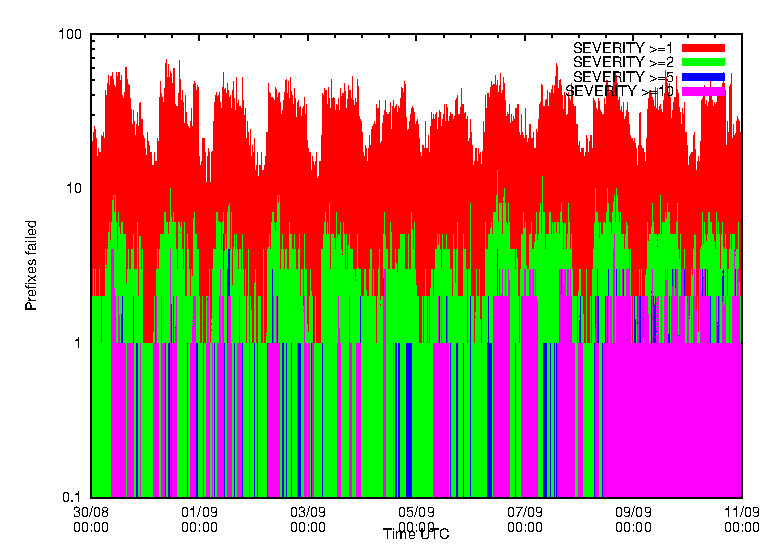
\includegraphics[height=8cm]{images/prefix_failed_ipv4.eps}\todo{replace image!}
	
	\vspace{3mm}
	
	Master Thesis MA-2012-11\\
	April 2012 -- October 2012\\
	
	\vspace{5mm}
	\begin{tabular}
		{l p{0.3
		\textwidth} l} \textbf{Advisors:} && \textbf{Supervisor:} \\
		Dominik Schatzmann && Prof. Dr. Bernhard Plattner\\
		Dr. Bernhard Ager && \\
	\end{tabular}
	
	\vspace{8mm} 
	\raggedleft 
	\begin{tabular}
		{rl} Communication Systems Group --& CSG\\
		Computer Engineering and Networks Laboratory --&TIK\\
		Department of Information Technology and Electrical Engineering --& ITET\\
		Swiss Federal Institute of Technology -- & ETH\\
	\end{tabular}
\end{titlepage} \cleardoublepage

\setcounter{page}{1} 
\pagenumbering{roman}

% Abstract


%!TEX root = ./main.tex
%%%%%%%%%%%%%%%%%%%%%%%%%%%%%%%%%%%%%%%%%%%%%%%%%%%%%%%%%%%%%%%%%%%%%%%%%%%%%%%
%%%%%%%%%%%   How to write an abstract  [1]       %%%%%%%%%%%%%%%%%%%%%%%%%%%%%
%%%%%%%%%%%%%%%%%%%%%%%%%%%%%%%%%%%%%%%%%%%%%%%%%%%%%%%%%%%%%%%%%%%%%%%%%%%%%%%
%
% ----------------------------------------------------------
% Goal:
%  1. ... "selling" your work
%  2. ... "selling" your work
%  3. ... "selling" your work
%
% ----------------------------------------------------------
% Checklist:
%
% Motivation:
% - Why do we care about the problem and the results?
% - Importance of your work, the difficulty of the area,
%   and the impact it might have if successful.
%
% Problem Statement:
% - What problem are you trying to solve?
% - What is the scope of your work ?
%
% Approach:
% - How did you go about solving or making progress on the problem?
% - simulation, analytic models, prototype construction?
%
% Results:
% - What's the answer?
% - is so many percent faster, cheaper, smaller, or otherwise better than something else
% - in numbers
% - talk about orders-of-magnitude improvement not small improvements!!!
%
% Conclusions:
% - What are the implications of your answer?
%
% Keywords:
% - ask your supervisor ...
%
%---------------------------------------------------------%
% Limits:
% - Word count limitation: 150 to 200
%
% [1] Philip Koopman, Carnegie Mellon University, 2007
%     How to Write an Abstract
%     http://www.ece.cmu.edu/~koopman/essays/abstract.html
%     10. Sept. 2007
%----------- FORMAT -----------------------------------------------------------
\clearpage \null 
\vfil 
\begin{center}
	\textbf{Abstract} 
\end{center}




\vspace{10em} 
\begin{center}
	\textbf{Keywords} \par 
\end{center}

%----------- FORMAT -----------------------------------------------------------
\vfil

\newpage
\clearpage \null 
\vfil 
\begin{center}
	\textbf{Abriss} 
\end{center}




\vspace{10em} 
\begin{center}
	\textbf{Schlüsselwörter} \par 
\end{center}

%----------- FORMAT -----------------------------------------------------------
\vfil


%
% Preface


%!TEX root = ./main.tex
%\clearpage
%\null
%\vfil
%---------- FORMAT -----------------------------------------------------------
\clearpage 
\begin{center}
	\textbf{Acknowledgments} 
\end{center}

During the creation of this thesis several people supported me. At this place, I would like to thank them.

At first, I am deeply grateful to Dominik Schatzmann and Dr. Bernhard Ager for their support, their great expertise and their patience in explaining me even basics concepts. They always asked the right questions at the right time, thus directing my focus on the important things. During the last half year, they always provided good remarks and excellent advisory -- not only regarding technical aspects. I really enjoyed the discussions and the process of working on this thesis with them. 

Furthermore, I would like to express my sincere gratitude to Prof. Dr. Bernhard Plattner for providing the opportunity to write this thesis in his research group and his excellent remarks. 

In addition, I enjoyed the support of the entire Computer Engineering Group (CSG) in various situations. In particular, I am grateful to Brian Trammell for always providing me the required support regarding the computing infrastructure in pleasant manner. 

Finally, I am very thankful to my close friends for motivating and supporting me in all circumstances.

%---------- FORMAT -----------------------------------------------------------
\vspace{1cm} Daniel Aschwanden 
\vfil

%---------- END -----------------------------------------------------------

%%% GLOSSARY %%%%
%!TEX root = ./main.tex

\newglossaryentry{botnet}{name=\oe botnet,
description={a network formed from bots},
plural=botnets,
sort=botnet}
\newglossaryentry{bot}{name=\oe bot,
description={computers compromised by malware that run automated tasks.},
plural=bots,
sort=bot}

% BGP
% IS-IS
% control-plane
% data-plane
% FACT
% ISP
% NAT
% Firewall

\printglossaries

\makeglossaries
\printglossary
\printglossary[type=\acronymtype,style=long3col]

\tableofcontents
\cleardoublepage

% Content
\pagenumbering{arabic} \setcounter{page}{1}

%!TEX root = ./main.tex
\chapter{Introduction\label{Introduction}}

% Problem: Connectivity problems exist
The end-to-end connectivity of hosts is one of the key services of the Internet. However, even after 40 years of intense engineering efforts, this connectivity is temporally broken for various reasons, such as link or hardware failure \citep{Markopoulou:2008}, mis-configurations \citep{Mahajan:2002}, or natural disasters \citep{Dainotti:2012:EBH,Schulman:2011}. 

% (Centrality Claim) Why do we care: Requires Troubleshooting Tools (TST) to minimize costs
This shows that there is a real need for methods to systematically detect and locate Internet outages of remote autonomous systems, subnets, and even single hosts. This is particularly true for \gls{isp}, because time intensive debugging sessions and the support of customers complaining at the \gls{isp} for unreachable networks are generating costs for the \gls{isp}. Occasionally, a \gls{isp} is even contractually liable for unreachable networks within the scope of a \gls{sla}. Therefore, an automated, ongoing detection and tracking of connectivity issues of the Internet may generate transparent outage information for customers and enables the \gls{isp} to react adequately on a detected reachability problems if possible, for example by changing routes in case of a failure of a transit provider. 

% (What is missing) Introduce the gap that we plan to close: 
Researchers and industrial vendors have proposed various approaches to systematically detect, locate and troubleshoot Internet outages due to the loss of end-to-end reachability. 

% State clearly what is missing
However, most of these approaches rely on \gls{control-plane} information such as \gls{bgp} routing messages or \gls{data-plane} information achieved by active probing. Both approaches are not perfectly suitable for practical usage.
% bash: control plane approaches & active probing approaches
As shown by \citet{Bush:Optometry}, packets in the Internet do not necessarily follow the \gls{control-plane} due to default routes or other secret peering policies. Moreover, connectivity issues imposed by packet filtering cannot be tracked by \gls{control-plane} approaches \citep{Dainotti:2011:ACI}. Besides legal issues, active probing requires the cumbersomeness of target selection and significantly increases the load on Internet infrastructure. Furthermore, there is still no active approach which scales well enough for the entire \gls{IPv6} address space. Moreover, both approaches are unable to track which part of the Internet is currently actively used by their internal clients. This is required to determine the amount of affected internal clients and therefore to assess the urgency of the outage event. For example, as long as a connectivity issue occurs within an unused remote network, the operator can handle this event with low priority and fix more urgent problems first.
To fill this gap, \citet{SchatzmannPAM2011} proposed the fully passive approach called \gls{FACT} relying on flow-level information to identify remote connectivity problems. The basic idea of \gls{FACT} is to match the corresponding outgoing and incoming flow to a bidirectional connection. Then, the remaining unidirectional connections or unresponsive connections are extracted and investigated. 

The detection of an outage is consolidated by aggregating these unresponsive connections to host, network and \gls{AS} level and rating the severity of the events by the number of affected internal users. This consolidation is required to reduce the noise of unresponsive connections caused by scanning or botnets and implies an implicit prioritization of events which affect many internal network users.

\citet{SchatzmanThesis2012} proposed to treat certain types of Internet services differently, because they do not require constant reachability. For example, Skype or BitTorrent applications that are often executed on client machines such as Desktops, Laptops, or Smartphones are likely to be reachable only for a limited time during a day.
This characteristic is caused by the fact that these machines are often disconnected from the network to save power or due to mobility effects. However, this temporal unreachability is not noticed as a problem by end-users. 
Therefore, issues of such client machine based services should not be treated the same way as server machine based services.

Currently, \gls{FACT} does not differentiate the kind of service for tracking connectivity issues. This leads to the problem that client based services which are designed to be temporarily unavailable are in the worst case incorrectly interpreted as network outage. At the moment, \gls{FACT} is dealing with this problem by three different approaches.

Firstly, \gls{FACT} monitors in a first step only traffic towards stable services. At the moment, this is heuristically defined by the traffic going to a remote \gls{TCP} port 80 traffic from an internal client high port, representing the assumption that this kind of traffic is destined for a legitimate and stable web server socket. This approach can be viewed as preselecting only the traffic destined for stable services.  

Secondly, a network is only declared as unreachable if and only if all connection endpoints located in this network are not responding resembling a kind of network based traffic aggregation. 

In addition, a detected network outage is rated by the number of internal users which are affected by this specific outage and thus prioritizing relevant network outages.

\begin{figure}
	[ht] \centering
	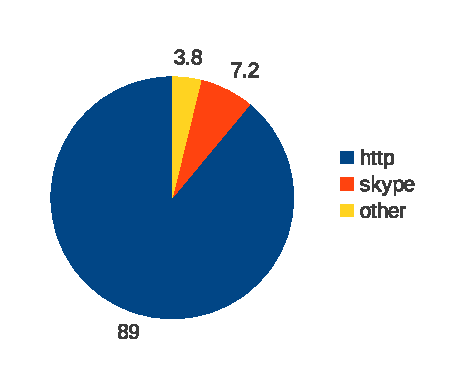
\includegraphics[width=6cm]{images/application_fact_port_80.eps}
	\caption{Application traffic running on TCP port 80 \citep{SchatzmanThesis2012}} 
	\label{fig:tcp_port80}
\end{figure}

However, by performing deep packet inspection \citet{SchatzmanThesis2012} has shown that the heuristic port based traffic preselection is not ideal, since a handful other applications are running on \gls{TCP}  port 80, presumably for firewall avoidance purposes. As shown in figure \ref{fig:tcp_port80}, the most relevant application running on \gls{TCP} port 80 -- besides \gls{HTTP} -- is Skype with a share of $7.2\%$ of all \gls{TCP} port 80 traffic. 

This \gls{TCP} port 80 based Skype traffic yields a completely different reachability characteristic. As shown by \citet{SchatzmanThesis2012}, there is a significantly higher amount of Skype \gls{TCP} port 80 sockets not reachable compared to \emph{normal} web server sockets of \gls{cdn} which is illustrated by figure \ref{fig:skype_traffic}. This exacerbates the reliable detection of network outages. 

\begin{figure}
	[ht] \centering
	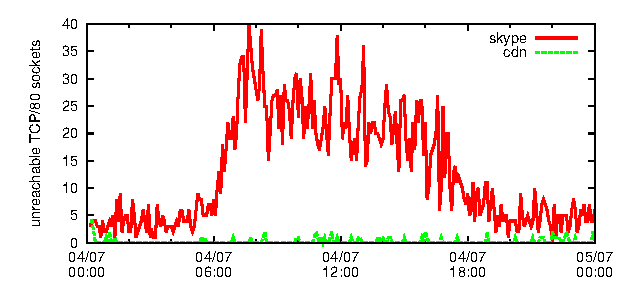
\includegraphics[width=12cm]{images/application_fact.eps}
	\caption{Unreachable TCP port 80 sockets differentiated by Skype and CDN application running on these sockets. \citep{SchatzmanThesis2012}} 
	\label{fig:skype_traffic}
\end{figure}

To this end, this thesis proposes a new type of traffic preselection which includes only traffic towards stable and reliable services. This is achieved by selecting traffic based on the past stability and popularity characteristics of remote services instead of the current heuristic port-based traffic preselection.

In detail, remote services are monitored and analyzed on longer time scales so that the deduced statistical information allows the characterization of the services. Consequently, only traffic towards sockets which are characterized as stable are monitored by \gls{FACT}. For example, a remote web server used only by few users that is often unreachable, e.g. due to testing or resource scarcity, should not be monitored by \gls{FACT}. In contrast, a popular content distribution host that was always reachable in the past is more relevant. 

To sum up, the overall goal of this thesis is to extend \gls{FACT} with a service monitoring and classification functionality to enhance the current rudimentary traffic preselection. In fact, this functionality should allow \gls{FACT} to focus even better on relevant connectivity issues which are related to stable and popular services.


\section{Related Work 
\label{sec:related_work}}
Due to the special interest of research and industrial vendors in the problem, there is a great effort done in the past. 
Generally, the related work with impact on this thesis can be separated into two thematically different topics.
On the one hand, there is a lot of research done in the area of reachability tracking. 
On the other hand, the topic of detecting network services is not only of interest for research and industry, but also for cyber criminals. 
In the following, both areas are briefly covered. 

\subsection{Reachability Tracking}

% Connection Tracking (Active & Passive)
Severe disruptions of the Internet's end-to-end connectivity is not a new phenomenon, there have been connectivity outages since its beginning as research project. 
Despite that the end-to-end connectivity is a very basic service of the Internet, the Internet community has not a deeply founded understanding of the problems that causes its disruption \citep{Bush:Optometry}.
A dominant share of researchers focussed on "pathological behavior related to the address space, e.g. bogon advertisements \citep{Feamster:2005}, prefix hijacking \citep{Zhang:2010}, \gls{bgp} misconfigurations \citep{Mahajan:2002} or \gls{DDoS} attacks \citep{Chen:2001}"\citep{Bush:Optometry}.

Basically, reachability can be viewed from two perspectives: \gls{data-plane} and \gls{control-plane} measurements. \citep{Feamster:2005,Zhang:2010,Mahajan:2002,Chen:2001} are mainly based on \gls{control-plane} information as publicly available BGP data for deducing knowledge about reachability. 
\citet{Bush:Optometry} pointed out that tracking \gls{data-plane} reachability with \gls{control-plane} information is heavily inaccurate due to the effect of secret peering policies, e.g., default routing. 
These allow packets to reach their destination even when a route failed to propagate through the \gls{bgp} system. 
\citet{Bush:Optometry} stated that even very basic \gls{data-plane} measurements
produce better views on reachability than \gls{bgp} observations. 
However, \gls{control-plane} based measurements are not limited to \gls{bgp} data, \citet{Markopoulou:2008} classified failures in a IP backbone network with \gls{is-is} information and tried to characterize these failures by layers as router, optical/link and maintenance. 
To sum up, \gls{control-plane} measurements of reachability are indirect and thus of limited practical usage for systematical reachability tracking approaches.

In contrast, measurements of the \gls{data-plane} are direct and can be more accurate regarding end-to-end connectivity. 
\Gls{data-plane} measurements can be divided into active probes and passive monitoring. 
Whereas active probes generates additional traffic towards the observed address space of the Internet, passive monitoring relies mainly on the traffic of servers and clients of the network or the traffic towards them. 

Active probing is widely used for end-to-end reachability problem detection, ranging from rudimentary debugging tools as ping \citep{PING}, paris traceroute \citep{traceroute} or nmap \citep{Nmap} to highly sophisticated, automated
outage detection tools as Hubble \citep{Katz:2008} or PlanetSeer \citep{Zhang:2004}. 
\citet{Bush:Optometry} pointed out that there exist some important limitations of active probing approaches as filtered packets by firewall and \gls{nat} devices or suboptimal routing which result in intermittent problems as packet rerouting.
Furthermore, there is no active probing technique known which is able to record the return path in addition to the forward-path which can be extracted for example with traceroute probes. 
It is not generally true to deduce that forward-path reachability implies return-path reachability as well, since there may be intermittent problems caused for example by suboptimal routing \citep{Bush:Optometry}.

% Pingin' in the rain (Schulman/Spring)
\citet{Quan12a} implemented an Internet outage detection engine which is able to actively probe a representative part of the Internet and correlate outage events with \gls{control-plane} information. 
This is achieved by a sophisticated target selection approach. 
However, this approach is avoiding some of the drawbacks of active probing as blockage by firewalls and \gls{nat} devices by clearly state that they are able to track the "analyzable" \gls{IPv4} address space of the Internet which represents the space which is answering on their active probes.
The future scalability of this approach -- especially with respect to \gls{IPv6} -- is questionable. 

%_--- PASSIVE --
Besides the big amount of different approaches using active probing, only few approaches are using passive monitoring for reachability tracking. 
\citet{Dainotti:2011:ACI} presented an approach for an in-depth analysis of connectivity outages caused by political censorship by combining observations from \gls{bgp} data, \gls{data-plane} information as backscatter measurements of the UCSD network telescope, and active probing measurements from the Archipelago Measurement Infrastructure. 
Remarkable is their approach of (passively) monitoring of the unsolicited \gls{data-plane} traffic that shed light on Libya's attempts on deploying packet filters for enforcing the Internet censorship. 
They concluded that this unsolicited and unwanted traffic captured by network telescopes may "illuminate many different types of macroscopic events, including but not limited to broad-scale packet-filtering-based censorship, which is not observable by \gls{bgp} data."\citep{Dainotti:2011:ACI}.

% evtl iatmon noch..
%\citet{SchatzmannPAM2011} aim to detect reachability problem by passively monitoring \gls{data-plane} measurement and aggregate unresponsive connection attempts on network- and AS-level.
\subsection{Service Detection} 

% Service Detection (Active & Passive, completeness vs. scalability / importance)
The discovery and characterization of services in the Internet is most successfully done on a massive scale, ironically not by researchers but by worms and other malware\citep{Chen:2007}. 
Generally, service detection methods can mainly be grouped into two approaches: passive monitoring and active probing. 
As \citet{Bartlett07b} pointed out, active probing is able to detect all visible and scannable services, which is thus invasive and legally constrained. 
On the other hand, passive monitoring is able to find transient services, but fails to detect idle services. 
In their work, they compared the "accuracy of passive and active approaches to service discovery and showed that they are complimentary"\citep{Bartlett07b}. 
They concluded that best results are achieved by combining a long lasting passive monitoring with multiple active scans, thus forming a hybrid approach\citep{Bartlett07b}. 

\citet{Leonard:2010} developed an Internet-wide service scanner called IRLscanner. 
They designed their scanner to maximize politeness to remote networks by smartly choosing adequate scanning rates. 

% Webster active / passive
\section{Contribution 
\label{sec:contribution}}
This master thesis contributions are the following: 
\begin{itemize}
	\item qualitative analysis of remote server sockets found by a passive approach based on \citet{Schatzmann:Mining,Schatzmann:Dissection, Schatzmann:Tracing} regarding their characteristics of stability, visibility and popularity.
	\item synthesis of the findings of this characterization for enhancing the traffic selection for tracking remote connectivity issues based on the approach of \citet{SchatzmannPAM2011}.
\end{itemize}

\section{Outline
\label{sec:outline}}



\todo{Write me at last..}


%!TEX root = ./main.tex
\chapter{Approach
\label{chapter:approach}}

To achieve the goal of enhancing the traffic preselection of \gls{FACT} with knowledge about the past stability and popularity characteristics, the following three steps are planned for extending \gls{FACT} as illustrated in figure  \ref{fig:FACT}.

In a first step, a network service detector (server socket detector) is  implemented. 
The challenge of the network service detection lies in the fact that the flow-level data does not provide enough precise timing information to determine which flow is originated from the client and thus making it impossible to deduce the server's socket \citep{Schatzmann:Tracing}. 
Therefore, the network service detection is achieved by the assumption that network services offered by servers act as concentrators in the sense that several clients have connections to this specific service. 
This approach bases on the work shown in \cite{Schatzmann:Dissection, Schatzmann:Mining, Schatzmann:Tracing} and is discussed in more detail in section \ref{section:socket_detection}.

\begin{figure}
	[t] \centering
	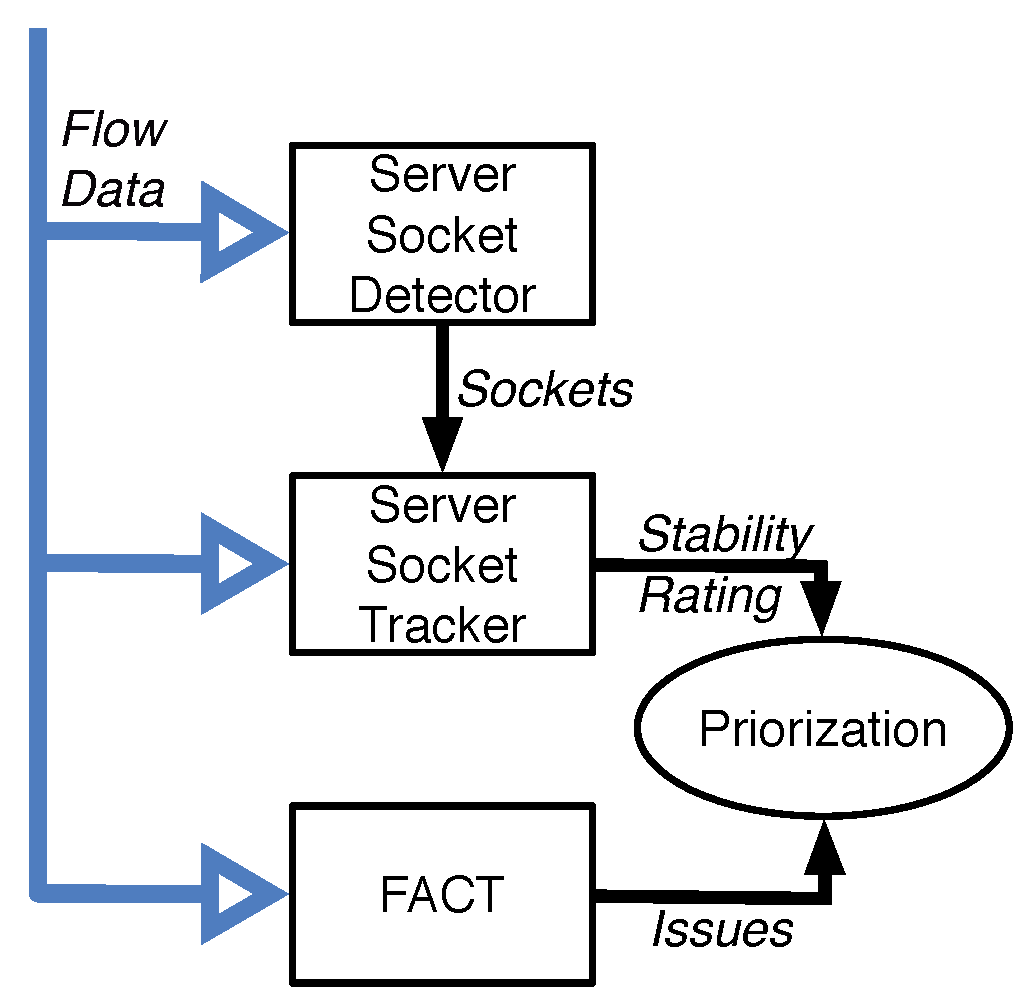
\includegraphics[width=8.5cm]{images/Approach_blockdiagram.eps}
	\caption{Interactions of new components with \gls{FACT}} 
	\label{fig:FACT} 
\end{figure}

In a second step, the previously detected network services are continuously  monitored. 
To provide information about the successful and unsuccessful connection attempts, a network service monitoring engine (server socket tracker) inspects all traffic towards these network services. This is covered in depth in section \ref{section:socket_tracking}.
Furthermore, these monitoring metrics are then used to statistically characterize the network services by their visibility, popularity and stability as further outlined in section \ref{section:characterization}.

In a third step, FACT is extended to use these server sockets to smartly preselect the traffic which should be monitored. 
This adaption is explained in section \ref{section:ses_traffic_selection}. 
By choosing a set of suitable network services, \gls{FACT}'s sensibility to events and the observation coverage can be increased. 
However due to performance reason, the number of network services which are observed by \gls{FACT} have to be reduced. 
To this end, the properties of these observation sets are assessed, because they influence the observation capabilities of \gls{FACT}. 
Particularly, the set's Internet address space coverage is a crucial property. 
With respect to FACT's goal of detecting remote network outages, it makes for example no sense to select only the most popular sockets if they are all located in the same network. 
Section \ref{section:ses_selection} is briefly discussing this problem.

%%%%%%%%%%%%%%%%%%%%%%%%%%%%%%%%%%%%%%%%%%%%%%%%%%%%%%%%%%%%%%%%%%%%%%%%%%%%%%%%
% SERVER SOCKETS
%%%%%%%%%%%%%%%%%%%%%%%%%%%%%%%%%%%%%%%%%%%%%%%%%%%%%%%%%%%%%%%%%%%%%%%%%%%%%%%%
\section{Server Sockets}
Since the Internet has moved from a research project to a widely used, public communication infrastructure, one of the critical success factors has been its diversity with respect to network applications or services. This has been heavily favored by the Internet's layered design as described by the \gls{osi}.

Todays network applications range from traditional services as web, \gls{FTP} or mail to relatively new and emerging services as video streaming and social networks. However, the terms \emph{network application} or \emph{network service} are overloaded and are used differently depending on the actual technical context.

By relying on flow-level data, information of layer 5-8 of the \gls{osi} model are not available in the data set. Therefore, network services can be differentiated only by information of layer 3 and 4 of the \gls{osi}. For this reason, the following abstractions of a connection end-point are defined:

%%%%%%%%%%% SOCKET DEFINITION 			%%%%%%%%%%%%%%%%%%%%%%
\parbox{
\textwidth}{
\begin{defn}
	{\textbf{Socket}\\} A socket is uniquely defined by the triple (\textbf{IP address}, \textbf{IP protocol number} and \textbf{protocol port number}). In this context, a socket is only defined for IP protocol 6 (\gls{TCP}) and 17 (\gls{UDP}).
\end{defn}
}
%%%%%%%%%%% SERVER SOCKET DEFINITION 	%%%%%%%%%%%%%%%%%%%%%%
\parbox{
\textwidth}{
\begin{defn}
	{\textbf{Server Socket
	\label{def:serversocket}}\\} A server socket is a socket with at least one process listening to incoming connections and thus offering a network service. The lifetime of a server socket is not restricted to individual connections, but by the lifetime of the network service.
\end{defn}
}

Despite of the use of the term \emph{server}, definition \ref{def:serversocket} is not only valid for classical server-client applications as \gls{HTTP}, \gls{FTP}, or \gls{SSH}, but also holds for \gls{p2p} applications. Furthermore, the definition allows completely symmetric server-server connections as for example \gls{NTP} as well. Due to reasons of completeness, the client socket is defined by definition \ref{def:clientsocket}. 

%%%%%%%%%%% CLIENT SOCKET DEFINITION 	%%%%%%%%%%%%%%%%%%%%%%
\parbox{
\textwidth}{
\begin{defn}
	{\textbf{Client Socket}\label{def:clientsocket}\\} A client socket is a socket which is only used to initiate and collate a connection to a server socket. Therefore, a client	socket is of temporary lifetime which is determined by the duration of the 	connection to the server socket.
\end{defn}
}


%%%%%%%%%%%%%%%%%%%%%%%%%%%%%%%%%%%%%%%%%%%%%%%%%%%%%%%%%%%%%%%%%%%%%%%%%%%%%%%%
% DETECTION OF SERVER SOCKETS
%%%%%%%%%%%%%%%%%%%%%%%%%%%%%%%%%%%%%%%%%%%%%%%%%%%%%%%%%%%%%%%%%%%%%%%%%%%%%%%%
\section{Detection of Server Sockets
\label{section:socket_detection}}

% problem of detection with flow-level information (timing issue + flags)
Basically, a \gls{server socket} can be identified due to the fact that a client opens a socket which initiates a connection to a \gls{server socket}. Usually, a \emph{client socket} port is chosen at random by its operating system and the \gls{server socket} port is statically allocated over the lifetime of network service process. Moreover, on each host a socket can only be assigned to one specific process per instance\footnote{Socket sharing techniques are not considered, because from a network point of view they are not of interest.}, i.e., an application can initialize a connection to a server socket and opens therefore a client socket, or a \glspl{server socket} network application is waiting for client connections on a specific socket. Otherwise, a socket-in-use-error is issued by the operating system \citep{Schatzmann:Dissection}.

A straight-forward approach for detecting \glspl{server socket} is to infer the initiator of the connection by the flow timing information and determine its opposite as the \gls{server socket}. 
However, this approach requires a perfect time synchronization of all flow exporting devices across the network. This is particularly true if there are asymmetric routes possible, such that packets can are recorded by several border routers.
In practice, this can be hardly achieved in a satisfactory and reliable way so that all occurring timing errors are corrected as shown by \citet{Trammell}.

% connection graph idea... +image
Besides the classification method based on well known ports, \citet{Schatzmann:Mining,Schatzmann:Dissection,Schatzmann:Tracing} proposed a heuristic, greedy approach for detecting \glspl{server socket} with flow-level data. The central idea of this approach is to build a bipartite communication graph, assuming that server sockets act as concentrators, and then to greedily solve a minimum vertex cover problem for extracting concentrators.

A bipartite connection graph as shown in figure \ref{fig:bipartite_graph}  consists of nodes, where each node represents an unique socket. If a bidirectional connection between two sockets is observed, an undirected, unweighted edge between the corresponding two nodes is assigned. This means that neither the direction nor the weight in terms of packets or bytes are required to build the connection graph.

\begin{figure}
	[h] \centering
	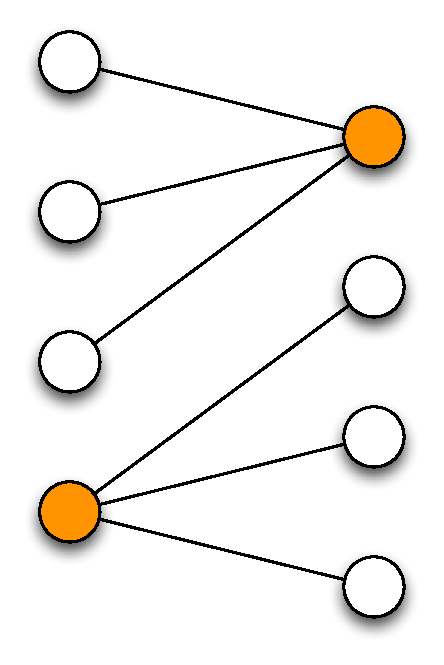
\includegraphics[width=\linewidth/3]{images/connection_graph.eps} \caption{Example of a bipartite connection graph with two concentrators of degree 3 marked as orange}
	\label{fig:bipartite_graph}
\end{figure}

Since \glspl{server socket} provide a network application or service, they are likely to be contacted by several clients depending on their popularity. To this end, a socket which is contacted by a certain amount of client sockets and thus has a high degree in the connection graph is defined to be a concentrator. These concentrators are likely to offer network services and are thus \glspl{server socket}. This approach is able to detect \glspl{server socket} which are offering not only classical client-server services running on well known ports, such as web, \gls{FTP}, or \gls{SSH}, but also \gls{p2p} applications such as for example Skype and Bit-torrent super-nodes.

Extracting the concentrators form the bipartite connection graph is basically a minimum vertex cover problem which can be solved by the greedy algorithm outlined in algorithm \ref{alg:service_tracing_ss-detection}. 
Generally, this algorithm creates two lists for each side of the graph, one list for the internal sockets and the other for the external. 
Both lists are sorted by the connection degree of the sockets. 
Then, the list with the higher degree is selected and their highest degree sockets are iteratively declared as concentrators and removed so that also all edges to other sockets are removed. 
After this step, both lists and their nodes are accordingly updated, especially all degrees of the remaining nodes. 
Then, the algorithm is repeated as long as there are nodes with higher degrees than $deg_{lim}$. 

% introduce minimal vertex cover problem
% greedy algorithm to solve mvcp
% recalling sockets for optimization
\begin{algorithm}[t!]
\caption{Detection of server sockets by \citet{Schatzmann:Mining,Schatzmann:Dissection, Schatzmann:Tracing}}
\label{alg:service_tracing_ss-detection}
\begin{algorithmic}
\STATE
\STATE compute list $SS_{in}$ \COMMENT{int. sockets sorted by \# ext. clients}
\STATE compute list $SS_{out}$ \COMMENT{ext. sockets sorted by \# int. clients}
\STATE
\WHILE{(deg($SS_{out}[0]$) $ > deg_{lim} $ \OR deg($SS_{in}[0]$)$ > deg_{lim}$)}
    \WHILE {(deg($SS_{in}[0]$) $ > $ deg($SS_{out}[0]$))}
        \STATE $ss$ = $SS_{in}[0]$ \COMMENT{classify $ss$ as internal server socket}
        \STATE remove $ss$ from $SS_{in}$
        \STATE update deg() for all entries of $SS_{in}$
    \ENDWHILE
    \WHILE{(deg($SS_{out}[0]$) $ \geq $ deg($SS_{in}[0]$))}
        \STATE $ss$ = $SS_{out}[0]$ \COMMENT{classify $ss$ as external server socket}
        \STATE remove $ss$ from $SS_{out}$
        \STATE update deg() for all entries of $SS_{out}$
    \ENDWHILE
\ENDWHILE
\end{algorithmic}
\end{algorithm}

\begin{figure}
	[ht] \centering
	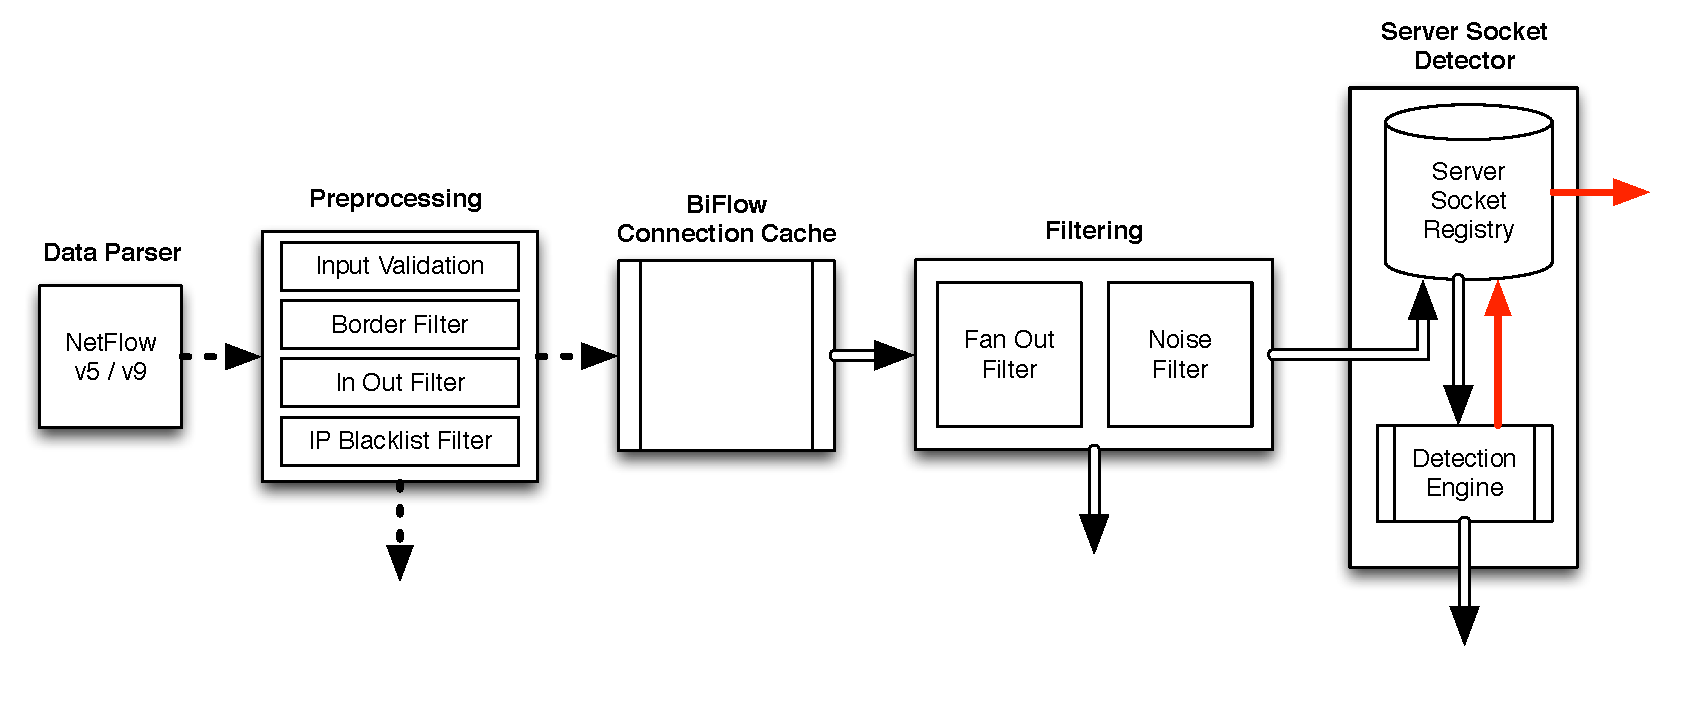
\includegraphics[width=\linewidth]{images/Detection_chain.eps}
	\caption{Processing chain for server socket detection}
	\label{fig:detection_chain}
\end{figure}

\subsection{Implementation}
Figure \ref{fig:detection_chain} illustrates the processing steps of the complete detection chain. The data parser is responsible to read the flow data either in the format of \gls{netflow} version 5 or \gls{netflow} version 9. These unidirectional flow records are then preprocessed by different blocks. While the input validator is performing some basic sanity checks of the flow data, the preprocessing filters are reducing the number of flows to the required kind of flow data.The border filter is removing all flow records not generated by a border router interface to efficiently prevent duplicate flow records. Then, the In-Out filter is removing all non cross-border traffic, i.e., transit traffic (external to external) or entirely internal traffic (internal to internal). Finally, the IP blacklist filter is removing traffic towards blacklisted IP addresses or networks.

After the preprocessing, the unidirectional flows are handed to the connection cache. This connection cache is responsible for merging all related unidirectional flow record into a single bidirectional flow record during a certain caching interval. 
Two unidirectional flows are related if the source socket of one flow record match the destination socket of another flow record and vice-versa\citep{Schatzmann:Tracing}. If there is for an unidirectional flow record no other related unidirectional flow, the flow is also transformed into a bidirectional flow. Although, this bidirectional flow consists only of a single direction. All the subsequent processing is done with bidirectional flow records which may be of unidirectional nature. 
Furthermore, since the subsequent data processing is clock-based, a caching period $T_{cache}$ and a export period $T_{exp}$ is defined such that every $T_{exp}$ seconds all bidirectional flows records active during the last $T_{cache}$ seconds are exported and deleted from the connection cache.

After this caching step, the bidirectional flows are filtered by a fan-out filter which implements the idea of \citet{Allman:2007} to mitigate the negative effects of scanning and \gls{p2p} churn on the detection approach. This scanning filter is discussed in more detail by \citet{Schatzmann:Mining,Schatzmann:Dissection,Schatzmann:Tracing}.

Afterwards, the remaining bidirectional flow records are again reduced by the noise filter. This last filtering module is responsible to filter bidirectional flow records which do not represent an actual bidirectional connection. A correct bidirectional connection is simply defined as either a correct \gls{TCP} handshake or a reply flow as in case of \gls{UDP}. Hence, the approach of deducing correct connections is to investigate the number of packets for each direction of the bidirectional flow record, i.e., the outgoing and the incoming flow record, since there are only cross-border flows remaining due to the In-Out filter. 
If a bidirectional \gls{TCP} flow has in a single direction less than 3 packets, the filter assumes that this flow does not represent a correct bidirectional connection and is removing this record. Accordingly, a bidirectional \gls{UDP} flow is required to consist of at least 1 packet for each direction. 

After these filtering steps, the remaining bidirectional flows are passed to the \emph{server socket detector} which is finally performing the \gls{server socket} detection approach previously discussed. 
Generally, the \emph{server socket detector} is built from two main parts. On the one side, there is the \emph{server socket registry} which is containing all already known \glspl{server socket}. 
On the other side, the detection engine implements the \gls{server socket} detection algorithm.

At first, the sockets of all bidirectional flows are queried against the current \emph{server socket registry} for checking if they are already known. 
If this is the case, the corresponding bidirectional flow records are removed and only the remaining flow records are passed to the detection engine to increase the efficiency of the detection algorithm. 
The detection engine builds the bipartite connection graph and is detecting the concentrators of it.
These detected \glspl{server socket} are then passed to the \emph{server socket registry} in order that these sockets may be recalled afterwards.

Finally, the \emph{server socket registry} is able to output all detected \glspl{server socket} of the observation period.

%%%%%%%%%%%%%%%%%%%%%%%%%%%%%%%%%%%%%%%%%%%%%%%%%%%%%%%%%%%%%%%%%%%%%%%%%%%%%%%%
% MONITORING OF SERVER SOCKETS
%%%%%%%%%%%%%%%%%%%%%%%%%%%%%%%%%%%%%%%%%%%%%%%%%%%%%%%%%%%%%%%%%%%%%%%%%%%%%%%%
\newpage
\section{Monitoring of Server Sockets
\label{section:socket_tracking}}

The previous section outlined the approach of detecting \glspl{server socket}. This section covers the approach of monitoring flow data and generating statistical information such that some characteristics and properties of the detected \glspl{server socket} can be assessed as further outlined in section \ref{section:characterization}.

\subsection{Server Socket Statistics}

Generally, during the monitoring steps all required information for characterizing the stability, visibility and popularity has to be captured. This kind of information is denoted as \gls{server socket} statistics.

To this end, all flows originating from a \gls{server socket} or flows which are destined to \glspl{server socket} are monitored for compiling these \gls{server socket} statistics. In contrast to the detection approach, all flows towards a known \gls{server socket} have to be considered, since they must be accounted into the statistics.

The flow-level data is usually discretely slotted into data bins of size of the export period $T_{exp}$. Therefore, for each \gls{server socket} a time series statistics record can be created. In detail, such a \gls{server socket} time series statistics record contains the following information:
\vbox{
\begin{itemize}
	\item number of bidirectional connections
	\item number of outgoing unidirectional connections
	\item number of incoming unidirectional connections
\end{itemize}
}

In a second step, these gls{server socket} time series statistics record can be aggregated in such a way that the information about the activity within a certain time slot is kept. Thus, such a aggregated gls{server socket} time series statistics record contains the following entries:

\vbox{
\begin{itemize}
	\item sum of bidirectional connections of each time slot
	\item sum of outgoing unidirectional connections of each time slot
	\item sum of incoming unidirectional connections of each time slot
	\item number of days with connections
	\item number of discrete time slots with connections
	\item timestamps of discrete time slots with connections
\end{itemize}
}

\subsection{Traffic Statistics}

Besides the individual \gls{server socket} statistics, overall traffic statistics are accounted as well. 
This allows to deduce knowledge of how good the monitoring capability of the \glspl{server socket} is. 
For this reason, each flow which belongs to a \gls{server socket} and is present in the \emph{server socket registry} is denoted as monitored. 
Otherwise, flows which do not belong to a \gls{server socket} are accounted as not monitored.

Moreover, all unmonitored flows can be further analyzed to gain a better understanding of the type of this unmonitored traffic. This can be done on one of the following three scopes:
\begin{itemize}
	\item protocol level
	\item port level for \gls{UDP} and \gls{TCP} flows
	\item location of the connection end-points
\end{itemize}

Since \glspl{server socket} are only defined for protocol \gls{TCP} and \gls{UDP}, all flows with another protocol are per definition unmonitored. The first scope captures statistics about these flows.

In a second step, there are statistics generated for all unmonitored \gls{TCP} or \gls{UDP} flows. 
There are various reasons for this kind of unmonitored flows, mainly related to the detection approach outlined in section \ref{section:socket_detection}. 
In most cases, the sockets are not contacted by enough clients, therefore, they are not detected as concentrators and in consequence of that not recognized as \glspl{server socket}. 
Furthermore, scanning activity is also a major contributor to these unmonitored flows, since scanning traffic and other non-legitimate traffic is removed before the \gls{server socket} detection is performed. 
Consequently, these scanned sockets are not detected as \glspl{server socket}, in case there is no legitimate traffic towards these sockets. 
Nevertheless, scanning traffic is considered in this monitoring phase as well.

On the one hand, there is the possibility to account for each port of the unmonitored flows which leads to very detailed statistical information.
However, this comes at the price of an inefficient processing and higher memory usage.

On the other hand, the flows can be categorized by port ranges. In the thesis at hand, there are just two ranges defined for this categorization:

\begin{itemize}
	\item low port: 0-1023
	\item high port: 1024-65365
\end{itemize}

These categories are further divided by the location of the socket (either internal or external) to involve the third scope as well. Hence, the unmonitored \gls{TCP} and \gls{UDP} flows are differentiated by the following four categories:

\vbox{
\begin{itemize}
	\item external port high, internal port high
	\item external port high, internal port low
	\item external port low, internal port high
	\item external port low, internal port low
\end{itemize}
}

All these general traffic statistics allow to deduce insights about the properties of the detection process by learning what is missed. 
Moreover, they reveal information about the properties of the current \gls{server socket} set with respect to traffic representation and thus about some properties of this set.

\subsection{Implementation}

Figure \ref{fig:monitoring_chain} shows the modular implementation of the \gls{server socket} monitoring chain. Comparing the monitoring chain with the detection chain from figure \ref{fig:detection_chain}, it is clearly visible that the modules up to the bidirectional connection cache are shared. 
However, in the monitoring chain there are no fan-out filter and noise filter applied. 
This is because every traffic destined to a \gls{server socket} should be considered.
Therefore, no bidirectional flow records are filtered before accounting them. 
The \emph{server socket monitor} is accounting the general traffic statistics as well as the individual \gls{server socket} statistics.

First of all, the bidirectional flow records are separated into those belonging to a known \gls{server socket}, denoted as monitored traffic, and those not belonging to known \gls{server socket}, denoted as unmonitored traffic. To be more precise, this is done by querying the \emph{server socket registry} which is loaded with previously detected \glspl{server socket}. Then, the traffic monitor investigates the monitored and unmonitored traffic for generating the overall traffic statistics.
Furthermore, it examines the unmonitored traffic even more closely for deducing knowledge about the other traffic statistic scopes like protocol, ports and location.

\begin{figure}[hb]
	\centering
	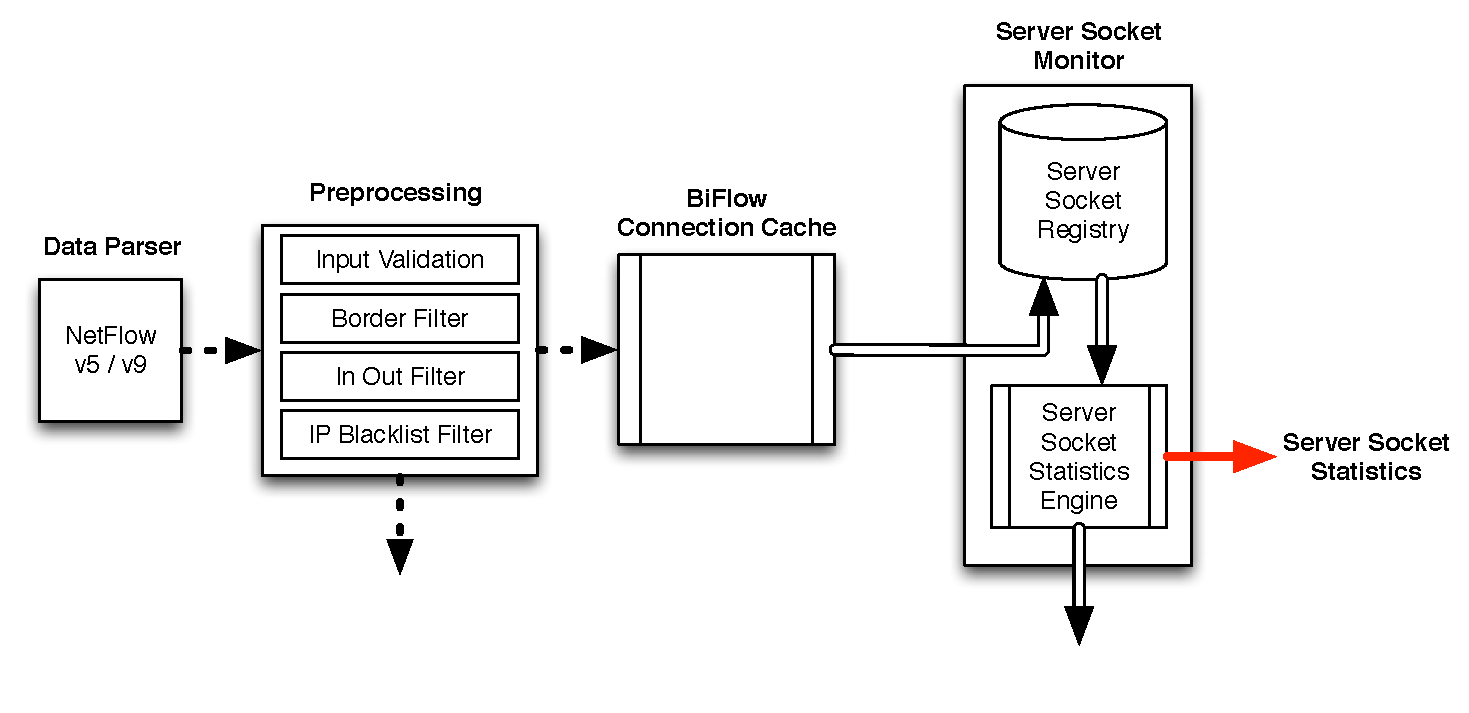
\includegraphics[width=\linewidth]{images/TrackingChain.eps}
	\caption{Processing chain for the server socket monitoring}
	\label{fig:monitoring_chain}
\end{figure}

%%%%%%%%%%%%%%%%%%%%%%%%%%%%%%%%%%%%%%%%%%%%%%%%%%%%%%%%%%%%%%%%%%%%%%%%%%%%%%%%
% CHARACTERIZATION SERVERSOCKETS
%%%%%%%%%%%%%%%%%%%%%%%%%%%%%%%%%%%%%%%%%%%%%%%%%%%%%%%%%%%%%%%%%%%%%%%%%%%%%%%%
\newpage
\section{Characterization of Server Sockets
\label{section:characterization}} 

The main interest of this thesis is to characterize \glspl{server socket} by their \textbf{stability}, their \textbf{visibility} and their \textbf{popularity}. These properties address the following characteristics of a \gls{server socket}:

\vbox{
\begin{itemize}
	\item \textbf{Stability:} How stable is the \gls{server socket} regarding its responsiveness or availability?
	\item \textbf{Visibility:} How frequently is the \gls{server socket} contacted?
	\item \textbf{Popularity:} How many distinct clients or sockets are contacting the \gls{server socket}?
\end{itemize}
}

These three characteristics are directly deducible from the statistics observed by the passive monitoring technique outlined in section \ref{section:socket_tracking}. In the following, the three characteristics are briefly discussed.

\subsection{Stability of a Server Socket}
According to the definition and the detection approach of a \gls{server socket}, it is offering a bidirectional service, which means that the client and the \gls{server socket} are both sending packets. 
Usually, a client socket is opening a connection to a \gls{server socket} which will reply then to this request. 
Generally, this also holds for \gls{p2p} applications as for example BitTorrent. Therefore, a \gls{server socket} -- or the communication of it -- can be characterized as stable if it responds to all connection attempts. 
If a connection attempt to a \gls{server socket} is answered by the \gls{server socket}, the connection is bidirectional, otherwise it is an unidirectional flow destined towards the \gls{server socket}.

Thus, the stability of a \gls{server socket} or availability of its service can be approximated by the ratio of the bidirectional flows to all flows destined to this \gls{server socket}, i.e., the bidirectional and the unidirectional incoming. 
This ratio is denoted as a \gls{server socket} \textbf{stability} and is mathematically defined by equation \ref{eq:ratio}.
\begin{equation}
	\text{Stability}(\text{Socket}_i) = \frac{\text{\#bidirectional flows}(\text{Socket}_i)}{\text{\#bidirectional flows}(\text{Socket}_i) + \text{\#unidirectional flows}_{in}(\text{Socket}_i)}
	\label{eq:ratio}
\end{equation}

A \gls{server socket} with a stability of 1 does only have bidirectional connections and thus, replies to all connection attempts. 
On the other hand, a stability of 0 indicates that there are only connections attempts by client sockets, but the \gls{server socket} has never replied upon these requests. 
Unidirectional outgoing connections from the \glspl{server socket} are indicating a client error or scanning activities of clients with spoofed (internal) source address which are not observed by the monitoring system. 
Therefore, these unidirectional outgoing connections are not considered for determining the stability ratio at all.

\subsection{Visibility of a Server Socket\label{subsection:visibility}}

% discrete time slots activities of a socket, per day, per 5min slot?
% distribution is heavy-tailed, alot of sockets only rarely connected => due to scanning? due to malware?
The monitoring process of the \glspl{server socket} is done passively. 
Thus, if a flow originating from a \gls{server socket} is visible in the flow-level data of a certain time period, the \gls{server socket} is active during a time interval $[t,t+\Delta{t}]$. 
Hence, the visibility of a \gls{server socket} is a binary measure, either inactive in case it is not visible or active in case it is visible in the data set. 
Equation \ref{eq:visibility} defines the visibility of a socket during the time interval $[t,t+\Delta{t}]$:
\begin{equation}
	\text{Visibility}_t(\text{Socket}_i,t+\Delta{t}) = \left\{
	\begin{array}{l l}
		1 & \quad \text{if $\text{Socket}_i$ is active during $[t,t+\Delta{t}]$}\\
		0 & \quad \text{if $\text{Socket}_i$ is not active during $[t,t+\Delta{t}]$}\\
	\end{array}
	\right.
	\label{eq:visibility}
\end{equation}

In consequence, there are different granularities $\Delta{t}$ to define the visibility of a \gls{server socket}. 
The most fine-grain resolution is the flow-level data cache export period $T_{exp}$. 
In most cases, this flow-level data cache export period $T_{exp}$ is set to 300 seconds. 
This most fine-grain resolution is referred to as the \emph{time slot} resolution, since the entire processing is based on such discrete data bins, which contains all active flows during this time period. 
Several more coarse-grain resolutions of the visibility might be of interest. For instance a resolution of a day, i.e., $\Delta{t} = 86400$s, is obvious.

Furthermore, the visibility of a \gls{server socket} can be extended from a single time period to the overall observation time, i.e., a week long trace, by summing up the individual visibilities of each time slot as shown in equation \ref{eq:visibility_sum}.

\begin{equation}
	\text{Visibility}(\text{Socket}_i) = \sum_{t} \text{Visibility}_t(\text{Socket}_i,t+\Delta{t})
	\label{eq:visibility_sum}
\end{equation}

However, this naive approach exacerbates the comparison between different observations since it represents the visibility in absolute terms. 
Therefore, a better metric for the visibility of a \gls{server socket} is to normalize the $\text{Visibility}_t(\text{Socket}_i,t+\Delta{t})$ as outlined by equation \ref{eq:visibility_avg}.
This ratio represents the average visibility of this socket in percent.
%This normalizes the visibility to a value in the range between 0 and 1, representing the ratio of its visibility to the maximum visibility possible. 
Thus, a value of 1 means that the socket is visible in every single time slot and a value of 0 that the socket is never active.

\begin{equation}
	\overline{\text{Visibility}}(\text{Socket}_i) = \frac{\sum_{t} \text{Visibility}_t(\text{Socket}_i,t+\Delta{t})}{\sum_{t}1}
	\label{eq:visibility_avg}
\end{equation}

\subsection{Popularity of a Server Socket}

% number of flows / clients?.. degree of Server Socket
Besides the visibility of a \gls{server socket}, its popularity is another major key characteristic. 
Whereas the visibility of a \gls{server socket} defines how frequent a socket is contacted by at least one connection endpoint, the popularity of a \gls{server socket} is defined by the number of connection attempts of client sockets during a certain period of time. 
The popularity of a \gls{server socket} can be deduced by various metrics such as the number of flows, bytes, or clients.

%%%%%%%%%%%%%%%%%%%%%%%%%%%%%%%%%%%%%%%%%%%%%%%%%%%%%%%%%%%%%%%%%%%%%%%%%%%%%%%%
% Smart Traffic Selection using Server Socket Sets
%%%%%%%%%%%%%%%%%%%%%%%%%%%%%%%%%%%%%%%%%%%%%%%%%%%%%%%%%%%%%%%%%%%%%%%%%%%%%%%%
\newpage
\section{Smarter Traffic Selection using Server Socket Sets 
\label{section:ses_traffic_selection}}

% explain briefly the approach / adjustments to FACT
Originally, \gls{FACT} applies a port-based heuristic for selecting the  examination traffic.  
In detail, \gls{FACT} selects in a first step all traffic towards an external  \gls{TCP} port 80 originating from an internal client high port. 
Generally, this kind of traffic is denoted as the reflector traffic. 
Then, \gls{FACT} examines each connection from the reflector traffic to determine if it is  bidirectional or unidirectional, thus creating an initial set of potential events of a reachability problem. 

\begin{figure}
	[!b] \centering
	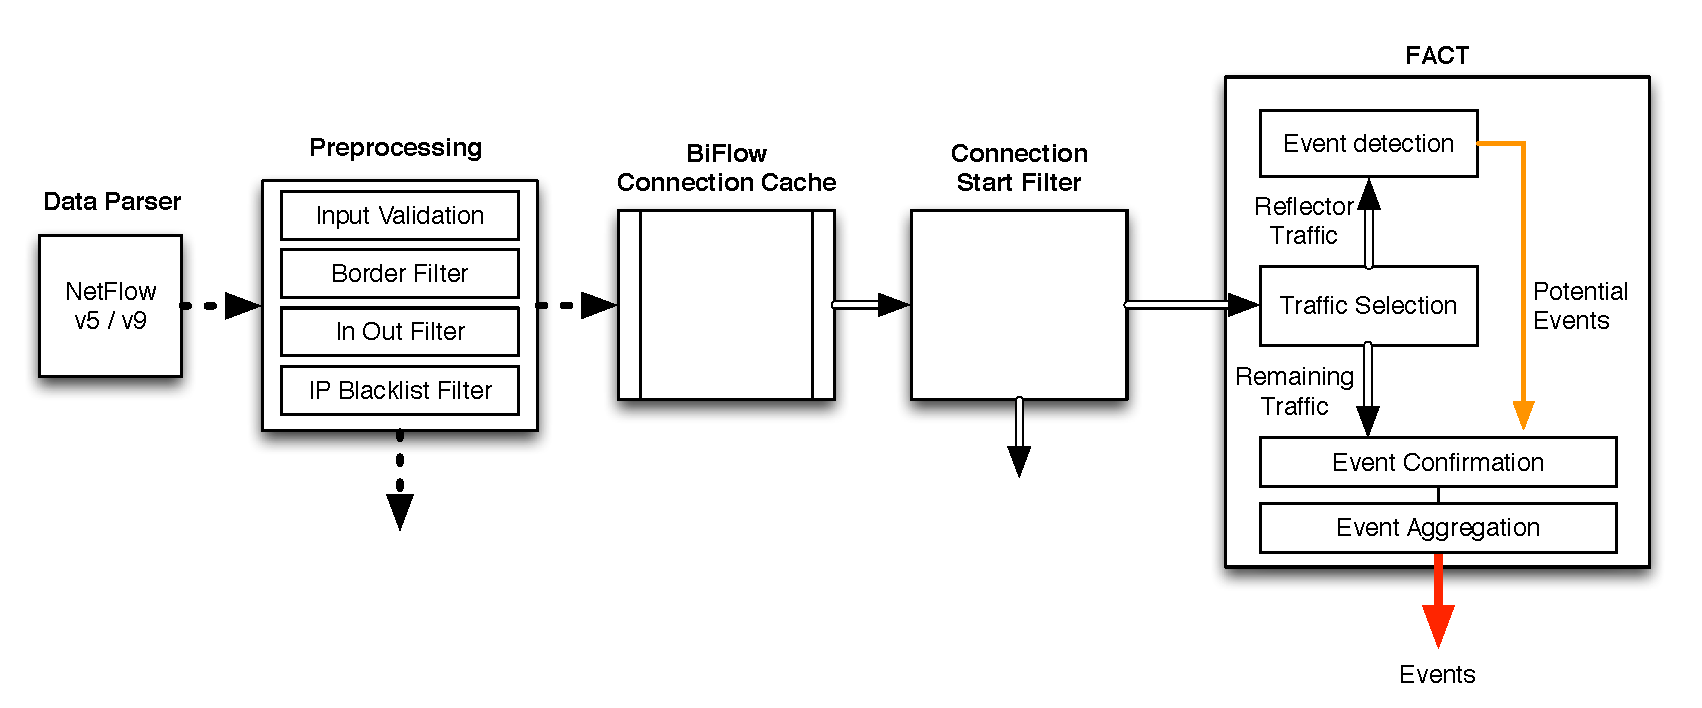
\includegraphics[width=\linewidth]{images/FACT.eps}
	\caption{Processing chain for FACT} 
	\label{fig:fact_chain} 
\end{figure}

In a second step, all potential events inferred by the reflector traffic are  double-checked with the remaining traffic if a potential event is indeed a  event. 
Only if there are no successful connections at all, i.e., all connections are unidirectional, a host, network, or prefix is declared as unreachable. 
Otherwise, if there is other traffic towards these hosts, networks, and prefixes with bidirectional connections, the potential event is obviously not confirmed and thus removed from the event list. 

Since the \gls{server socket} approach aims to replace the port-based heuristic,  only the generation of the reflector traffic set must be adjusted. 
The further processing steps remain exactly the same. 
Figure \ref{fig:fact_chain} illustrates the \gls{FACT} processing chain and makes clear that only the block of the traffic selection must be adjusted to examine traffic towards \glspl{server socket} as reflector traffic. 
This is achieved by loading the \gls{server socket} registry with a set of \glspl{server socket}. 
Then, the adjusted traffic selection is querying the server socket registry to determine if the external socket is a known \gls{server socket}. 
If this is the case, the flow is added to the reflector traffic, otherwise to the remaining traffic. 

\subsection{Selecting Suitable Server Socket Sets\label{section:ses_selection}}
% outline that this is a optimization problem which is approximated by several 
% socket sets however not guaranteed to be optimal
% coverage network space / problem space 
By replacing the original the traffic selection of \gls{FACT} with \gls{server socket} sets,  some essential properties of \gls{FACT}, like the observed network coverage or the event sensibility are directly dependent on properties of the chosen \gls{server socket} set. 

Because \gls{FACT} detects only network outage events which are firstly detected  with the reflector traffic and then not whitelisted by the remaining traffic, it  is able to detect only network outages of prefixes which have at least one known  server socket that is located in this prefix. This means that FACTs observation  coverage of networks is completely defined by the network/prefix coverage of the  chosen \gls{server socket} set. 

Obviously, it makes no sense to select for example the 10 most popular sockets if they are all located in the same network and prefix, because this set would just achieve a network coverage of 1 network/prefix. 
Hence, the network coverage can be optimized by selecting the best socket of these 10 and then select 9 different sockets which are all located in different networks/prefixes. 
By doing so, the network coverage can be increased. However, if a selected  \gls{server socket} is not contacted during an observation period the observation coverage of this network is lost, unless there is another contacted socket located in this network. 
This shows that the selection of \glspl{server socket} is cumbersome and directly influences the observation capabilities of FACT. It also shows the importance of the visibility and popularity characteristics of \glspl{server socket} with respect to the selection in a \gls{server socket} set. 

A popular \gls{server socket} which is always contacted by at least one client is able to cover the entire network, because even if this socket is not reachable during an observation period the network is further investigated by the remaining traffic. 
This is because the unidirectional connection of this \gls{server socket} will trigger a potential event which is then confirmed or whitelisted by the  remaining traffic towards this network. 
Otherwise, if a socket is not popular and only rarely visible, it will not generate a potential event, and hence, the event is not detected at all, even if there is a lot of unidirectional traffic towards this network contained in the remaining traffic. 

Therefore, the selection of the \glspl{server socket} is basically an optimization problem. 
The goal is to select those sockets with good stability, popularity and visibility characteristics without loosing to much network coverage. 
This problem can even be harder if the number of sockets is limited, then the socket density of each network must be considered, so that only the few best sockets located in a single network are selected.
It can even make sense to include not perfectly 
stable sockets if they increase the network coverage, especially if they have a good visibility and popularity.

%!TEX root = ./main.tex
%** Results.tex: What were the results achieved including an evaluation
\chapter{Results and Evaluation \label{chapter:results}}

This chapter covers an analysis of server sockets detected and an evaluation of the modified traffic preselection of \gls{FACT} and its effect on the event detection. 
Section \ref{section:analysis_in_wild} covers the a detailed analysis of a one-week long monitoring of server sockets. Their statistical characteristics with respect to stability, visibility and popularity are examined. 
The data used for this analysis is briefly described in section \ref{section:data}.
In section \ref{section:enhanced_FACT_eval} an evaluation of the adjusted traffic preselection of \gls{FACT} based on server sockets and its effect on \gls{FACT}'s observation capabilities is done.
Finally, section \ref{section:results} briefly summarizes the main findings of this chapter. 

%%%%%%%%%%%%%%%%%%%%%%%%%%%%%%%%%%%%%%%%%%%%%%%%%%%%%%%%%%%%%%%%%%%%%%%%%%%%%%%%
% DATA
%%%%%%%%%%%%%%%%%%%%%%%%%%%%%%%%%%%%%%%%%%%%%%%%%%%%%%%%%%%%%%%%%%%%%%%%%%%%%%%%
\section{Data 
\label{section:data}}

This evaluation relies on data collected at \citet{switch}, the Swiss National Research and Education Network (NREN). 
Mainly government institutions, universities, research labs are connected to the Internet by \citet{switch}\citep{Schatzmann:Mining}.

The \citet{switch} network is with approximately 250'000 network users in 2010 comparable with a mid sized \gls{isp}. Currently, there are around 2.4 million \gls{IPv4} addresses, a /32 IPv6 and a /40 \gls{IPv6} network announced via \gls{bgp}\citep{Schatzmann:Tracing}.
\begin{figure}
	[ht] \centering 
	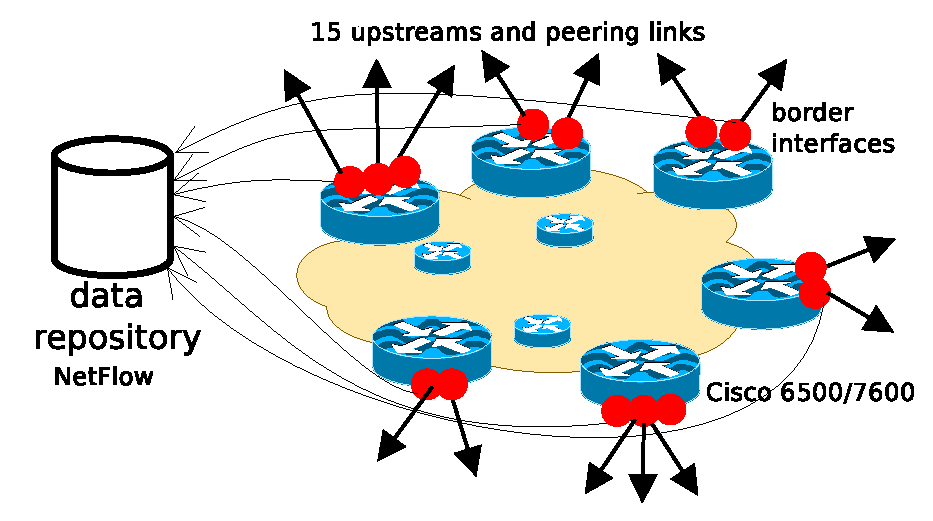
\includegraphics[width=12cm]{images/network_overview.eps} \caption{Overview of the SWITCH network \citep{SchatzmanThesis2012}} 
	\label{fig:switch_nework} 
\end{figure}

Figure \ref{fig:switch_nework} provides an overview of the SWITCH network. 
Currently, SWITCH has 15 upstream and peering links and is capturing flow level data at all external interfaces of their border routers. From 2003 to 2008 \gls{netflow} version 5 has been used, and \gls{netflow} version 9 after 2008\citep{Schatzmann:Tracing}.

High traffic peak rates of more than 80'000 flows per second, 3 million packets per second and more than 20Gbit/s require hardware-based flow collection cards\citep{Schatzmann:Tracing}. 
\gls{TCP} flags are not available in the flow-level information because of limitations of the used hardware components\citep{Schatzmann:Tracing}. 
The generated flow data are collected and stored in a central data repository.

% briefly describe the Switch network and its topology..
% traffic volume and netflow data unsampled!
% see tech report 338 for numbers and layout?! evtl actual numbers (2012)
%%%%%%%%%%%%%%%%%%%%%%%%%%%%%%%%%%%%%%%%%%%%%%%%%%%%%%%%%%%%%%%%%%%%%%%%%%%%%%%%
%%%%%%%%%%%%%%%%%%%%%%%%%%%%%%%%%%%%%%%%%%%%%%%%%%%%%%%%%%%%%%%%%%%%%%%%%%%%%%%%
% ANALYSIS of SERVER SOCKETS IN THE WILD
%%%%%%%%%%%%%%%%%%%%%%%%%%%%%%%%%%%%%%%%%%%%%%%%%%%%%%%%%%%%%%%%%%%%%%%%%%%%%%%%\newpage
\section{Analysis of Server Sockets in the Wild\label{section:analysis_in_wild}}

This section covers an analysis of \gls{server socket} found during a week long data trace from 2010/11/01 00:00:00 UTC until 2010/11/06 00:49:00 UTC, thus covering mainly the first 5 working days in November 2010.

\subsection{Detected Server Sockets}

% sum up of detection parameters > 2 biflows per 5min interval with more TCP
% packets > 3 UDP > 1
For detecting the \glspl{server socket} in this observation period, the previously discussed detection approach is applied as illustrated by figure \ref{fig:detection_chain}. 
In detail, the connection cache was configured with a cache interval of 600 seconds and an export interval of 300 seconds. Hence, all flows active during the last 600 seconds are exported every 300 seconds. The cache interval of 600 seconds is chosen according to \citet{Schatzmann:Tracing} for making it likely to observe at least some flows to any active server socket. 

%to summarize all related unidirectional flow records into a single bidirectional flow record during an aggregation interval of 600s.
After this caching step, the bidirectional flows are filtered by a fan-out filter implementing the idea of \citet{Allman:2007} to mitigate the effects of scanning and \gls{p2p} churn. 
This fan-out filter is configured to require at least 4 unidirectional connections with a certain host as source and at least 2 times more unidirectional connections than bidirectional connections for classifying this host as a scanning host. 
Previous work\citep{Schatzmann:Mining,Schatzmann:Dissection, Schatzmann:Tracing} has shown that these parameters are a good choice for efficiently mitigating the scanning noise so that the scanning spikes of the total traffic volume are successfully reduced.

Moreover, the noise filter is configured to filter all bidirectional \gls{TCP} flows with less than 3 packets in a single direction and bidirectional \gls{UDP} flows which are actually unidirectional flows and have 0 packet in a single direction.

Furthermore, the \emph{server socket detector} is configured to extract sockets with a degree of 2 or higher as concentrators, thus requiring two independent connections to a \gls{server socket} within 600 seconds.

% state overall number of detected external and internal server sockets during
% this period
During the entire observation period of 120.8 hours, the \emph{server socket detector} managed to detect 1'862'389 external \glspl{server socket} and 609'670 internal \glspl{server socket}.

\subsection{Traffic Attraction of Server Sockets}

% traffic statistics of server sockets detected by type and ratio of traffic
% towards server sockets
In the following, the overall traffic statistics of the detected \glspl{server socket} are briefly discussed. Figure \ref{fig:flows_by_type} shows the absolute number of flows during the entire observation period separated by the type of connection. 
If the flow is destined to a \gls{server socket}, the flow is denoted as monitored, otherwise as unmonitored. 
Furthermore, the type of connection also considers the direction of the connection, i.e., if the flow is bidirectional, unidirectional outgoing or unidirectional incoming. 
Hence, in total there are six possible combinations for the type of connection, allowing a good interpretation of the detection approach. 
For easier comparison of each type of connection, figure \ref{fig:monitored_flows_by_type} shows the ratio of monitored and unmonitored flows by the direction.

In figures \ref{fig:flows_by_type} and \ref{fig:monitored_flows_by_type}, there are two gaps visible around 2010/11/01 10:00 UTC and 2010/11/04 06:05 UTC. 
These gaps result from missing flow records resulting from router reboots, collector outages, and storage failures\citep{Schatzmann:Mining}.
\begin{figure}
	[ht] \centering 
	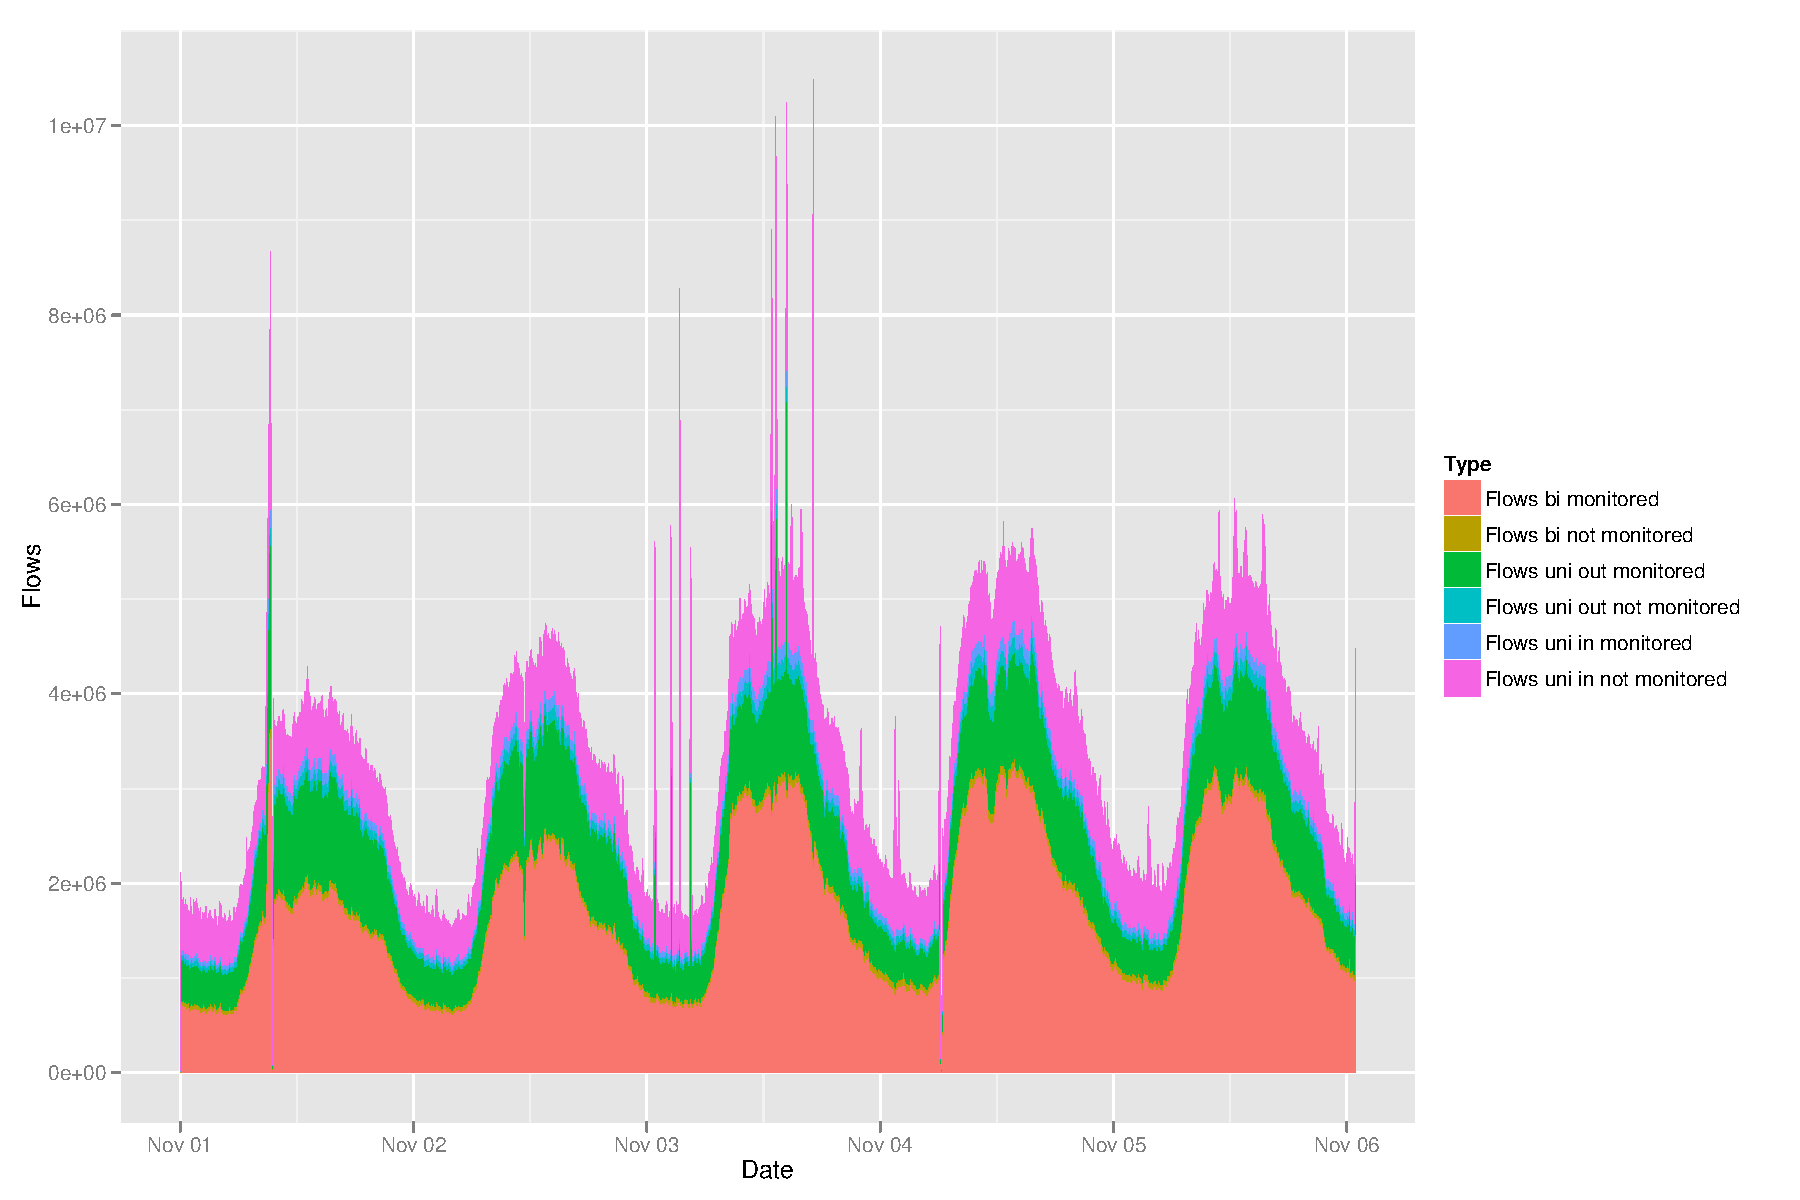
\includegraphics[width=\linewidth]{images/Flows_by_type_area_all_SeS.pdf} \caption{Number of flows over time by the type of connection with all detected server sockets} 
	\label{fig:flows_by_type} 
\end{figure}
\begin{figure}
	[h] \centering 
	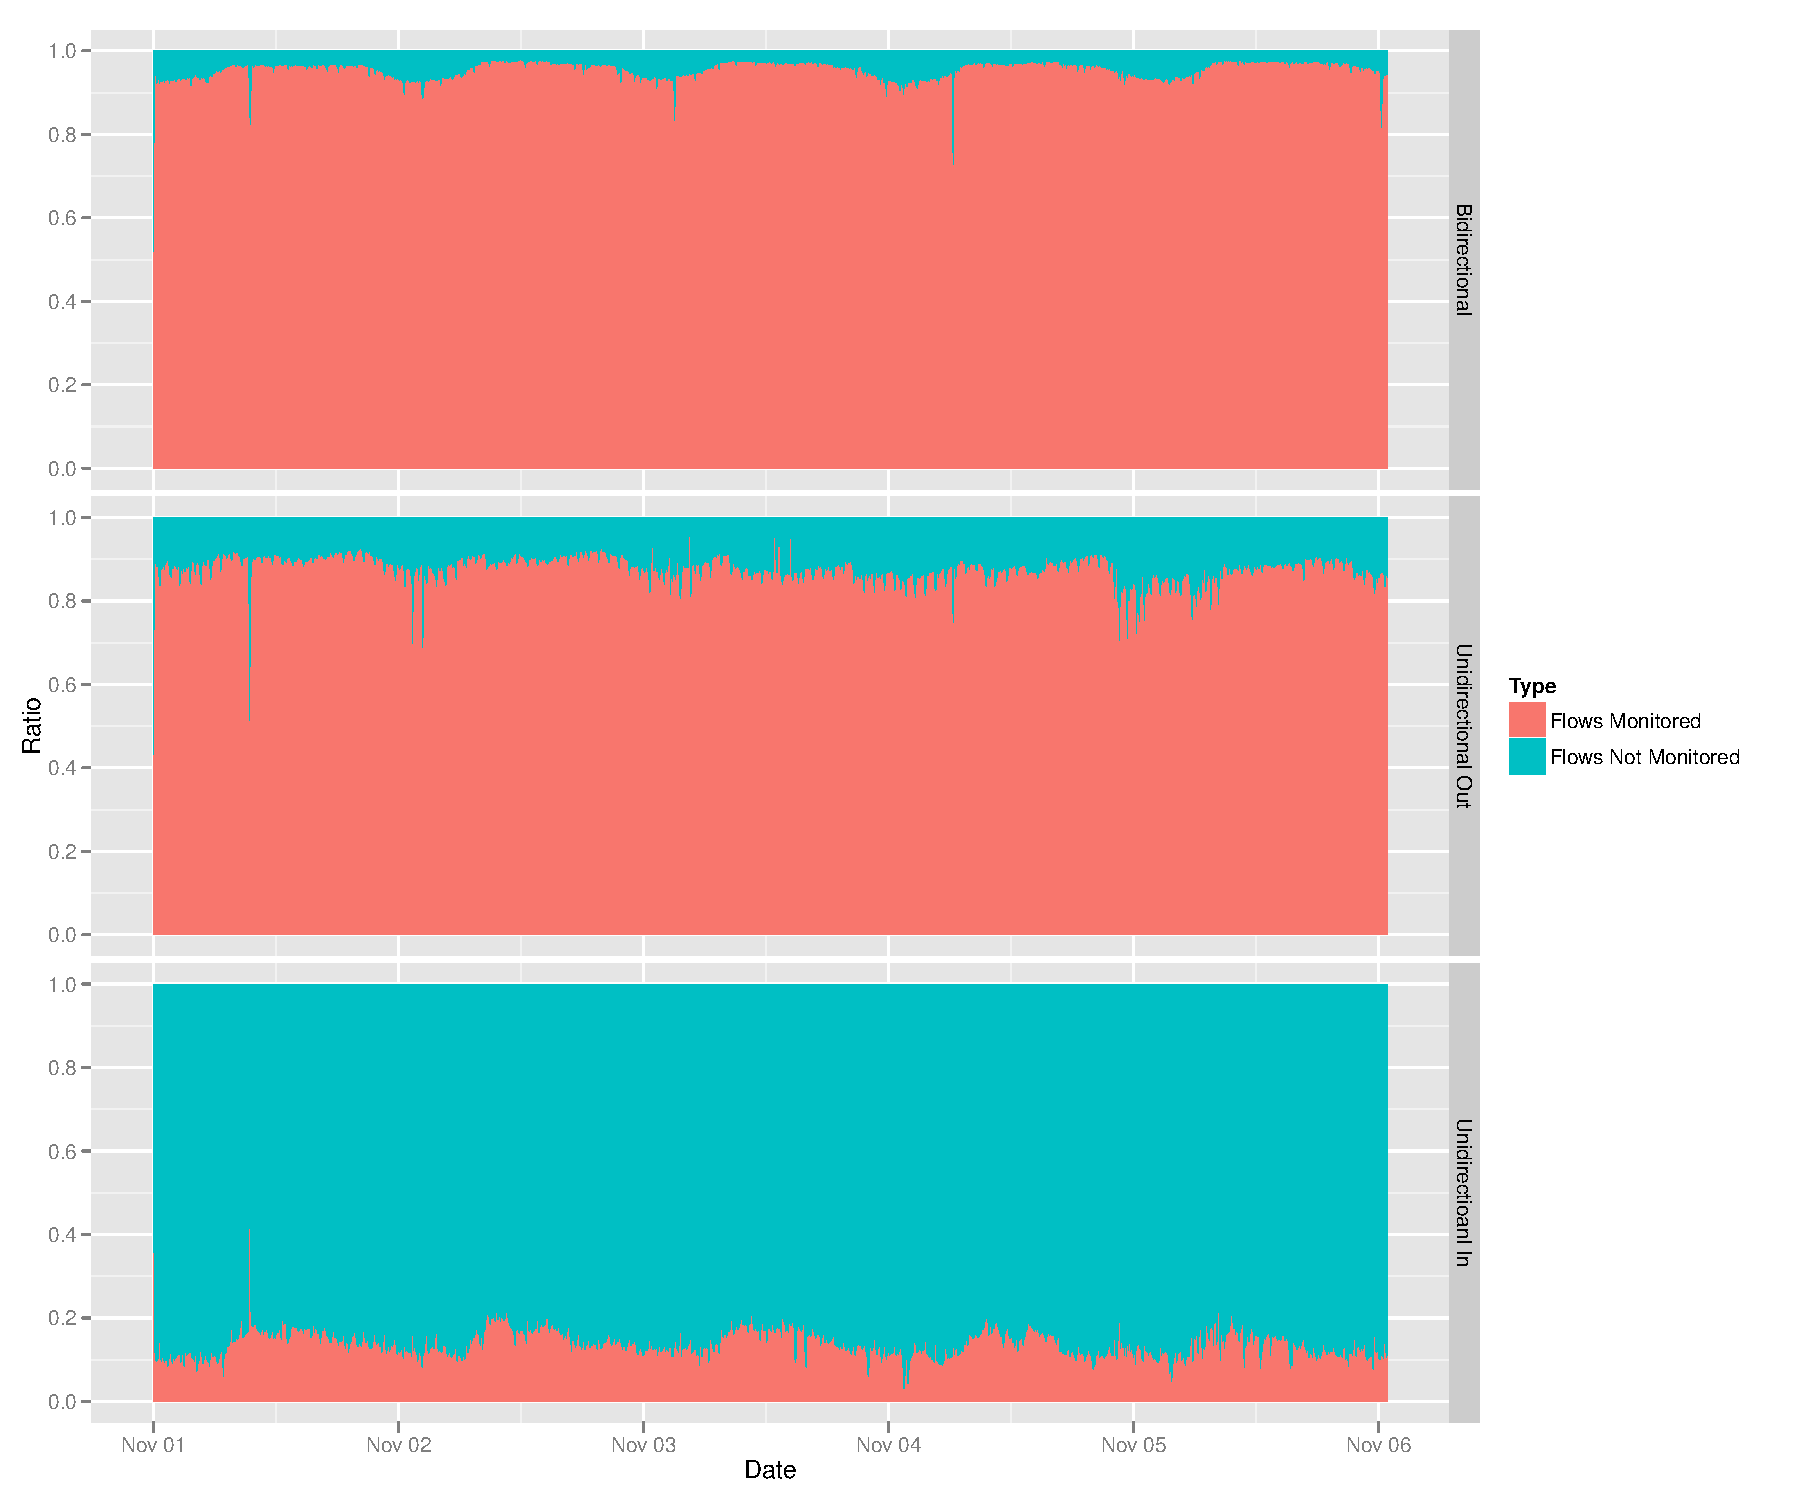
\includegraphics[width=\linewidth]{images/Flows_monitor_ratio_by_type_all_SeS.pdf} \caption{Flows towards known server sockets by traffic type with all detected server sockets} 
	\label{fig:monitored_flows_by_type} 
\end{figure}

Clearly, the dominating kind of flows are the bidirectional monitored flows represented by the red area in figure \ref{fig:flows_by_type}. 
Comparing this share with the bidirectional unmonitored flows represented by the hardly visible black area between the red and the green area, yields that the detection approach successfully detects a majority of the \glspl{server socket} from the bidirectional traffic. 
This finding is even better visible on the bidirectional ratio of figure \ref{fig:monitored_flows_by_type}. 
Depending on the time of the day, the monitoring ratio of the bidirectional flows is mainly between 90\% and 97\%. 
The smaller monitoring ratios during night indicates that there is a higher share of unknown \glspl{server socket} active at night than during day. 
A possible reason for pattern is that there are some \glspl{server socket} which are regularly contacted, although, only by very few clients so that these sockets get never more than one connection within 600 seconds. 
Thus, these sockets are never detected as concentrators.

Similarly, if the unidirectional outgoing flows are examined by looking at figure \ref{fig:monitored_flows_by_type}, the monitored flows have predominantly a high share of around 80\% to 90\% of all unidirectional outgoing flows. 
Figure \ref{fig:flows_by_type} also reveals some high peaks which are probably scanning or backscatter effects which are well visible at November 03 in the night and in the afternoon by the green spikes. 
However, these green peaks are categorized as monitored unidirectional outgoing flows. 
Thus, they must involve at least one known \gls{server socket} either located external or internal.

Finally, the unidirectional incoming flows are predominately unmonitored with around 80-97\% of unmonitored flows as it can be seen in figure \ref{fig:monitored_flows_by_type}. 
The main reason for this contrast may be that the main part of this unidirectional incoming traffic consists of Internet background radiation \citep{Wustrow10,Pang04} resulting from malware or misconfiguration for example. 
Nevertheless, this unidirectional incoming traffic is unimportant with respect to the scope of this thesis.

To sum up, \glspl{server socket} tend to attract a majority of the observed connections, especially the bidirectional connections and the unidirectional connections which are important to the connectivity tracking. 
Therefore, they are well suitable to represent the legitimate traffic which is indeed interesting for tracking the end-to-end connectivity.

%In a metaphorical sense, \glspl{server socket} are comparable to masses in physics which are exerting gravitational forces to other objects. 
%\Glspl{server socket} tend to attract a majority of the observed connections. 
%Therefore, they are well suitable to represent a majority of the legitimate traffic which is interesting for tracking the end-to-end connectivity.
\newpage 
\subsection{Characterization of Detected Server Sockets}

As discussed in section \ref{section:characterization}, this thesis proposes to characterize \glspl{server socket} according to their visibility, popularity and stability by different metrics. This section aims to deduce some statistical properties of these characteristics for the detected \glspl{server socket}.

\subsubsection{General Visibility of Server Sockets}

For defining a metric of the visibility of \glspl{server socket}, it is required to define the granularity of a observation period according to \ref{subsection:visibility}. For simplicity reasons, only two different granularities are defined.

One the one hand, a day long observation period yields the number of visible days for the activity of a socket. 
On the other hand, an observation period of 5 minutes is chosen, since it reflects the default processing interval of FlowBox and the native caching interval of the flow data. 
This allows a very fine-grained, detailed resolution of a \glspl{server socket} activity. 
This second visibility metric is referred as \emph{visible time slots(VTS)}.
\begin{figure}
	[hb] \centering 
	\includegraphics[width=\linewidth]{images/VTS_by_visibledays.pdf} \caption{Each of the six histograms shows the number of sockets by visible time slots for each value of visible days} 
	\label{fig:vts_by_visibledays} 
\end{figure}

Figure \ref{fig:vts_by_visibledays} shows six histograms. Each of the histograms shows the visible time slots of the sockets separated by their daily visibility. This means that the histogram of all sockets with a daily visibility of 1 day is the top left diagram. The skewness of the distributions for 1 to 4 visible days are is very similar. 
It is obvious that the a socket which is visible for only one day cannot exceed 288 visible time slot. 
Nonetheless, considering this daily scaling factor, the distributions are looking very similar. 
Furthermore, figure \ref{fig:vts_by_visibledays} shows that the most sockets in absolute terms are only active during one day and only in very few visible time slots.

However, the distribution of the number of sockets with a visibility of 5 or even 6 days are slightly different, since there is a higher share of sockets with a relatively higher visible time slots, besides the normal scaling factor of the number of visible days.

This is an important finding, because connectivity tracking requires sockets which tend to be often visible. Hence, with different visibility criteria those are easily extractable. 

\subsubsection{Visibility and Stability} Eventually, for selecting those \glspl{server socket} which are stable and often visible it is of importance to assess how \glspl{server socket} are distributed with respect to their stability and visibility characteristic. 
Hence, figure \ref{fig:rankedVisibility} shows the quantile of the visible time slot of each socket and their stability. 
Thus, a socket with a visibility quantile of 80\% indicates that there are 80\% of all sockets with the same or lower visibility than this specific socket.

As figure \ref{fig:rankedVisibility} indicates, the sockets cluster around the top right corner, hence the top visible sockets tend to have a good stability as well. This is important with respect to the intent to use the server sockets for connectivity tracking. For this purpose, sockets which are stable and often visible are required which are indeed located in the cluster on the top right of figure \ref{fig:rankedVisibility}.
 
\begin{figure}[ht] \centering 
	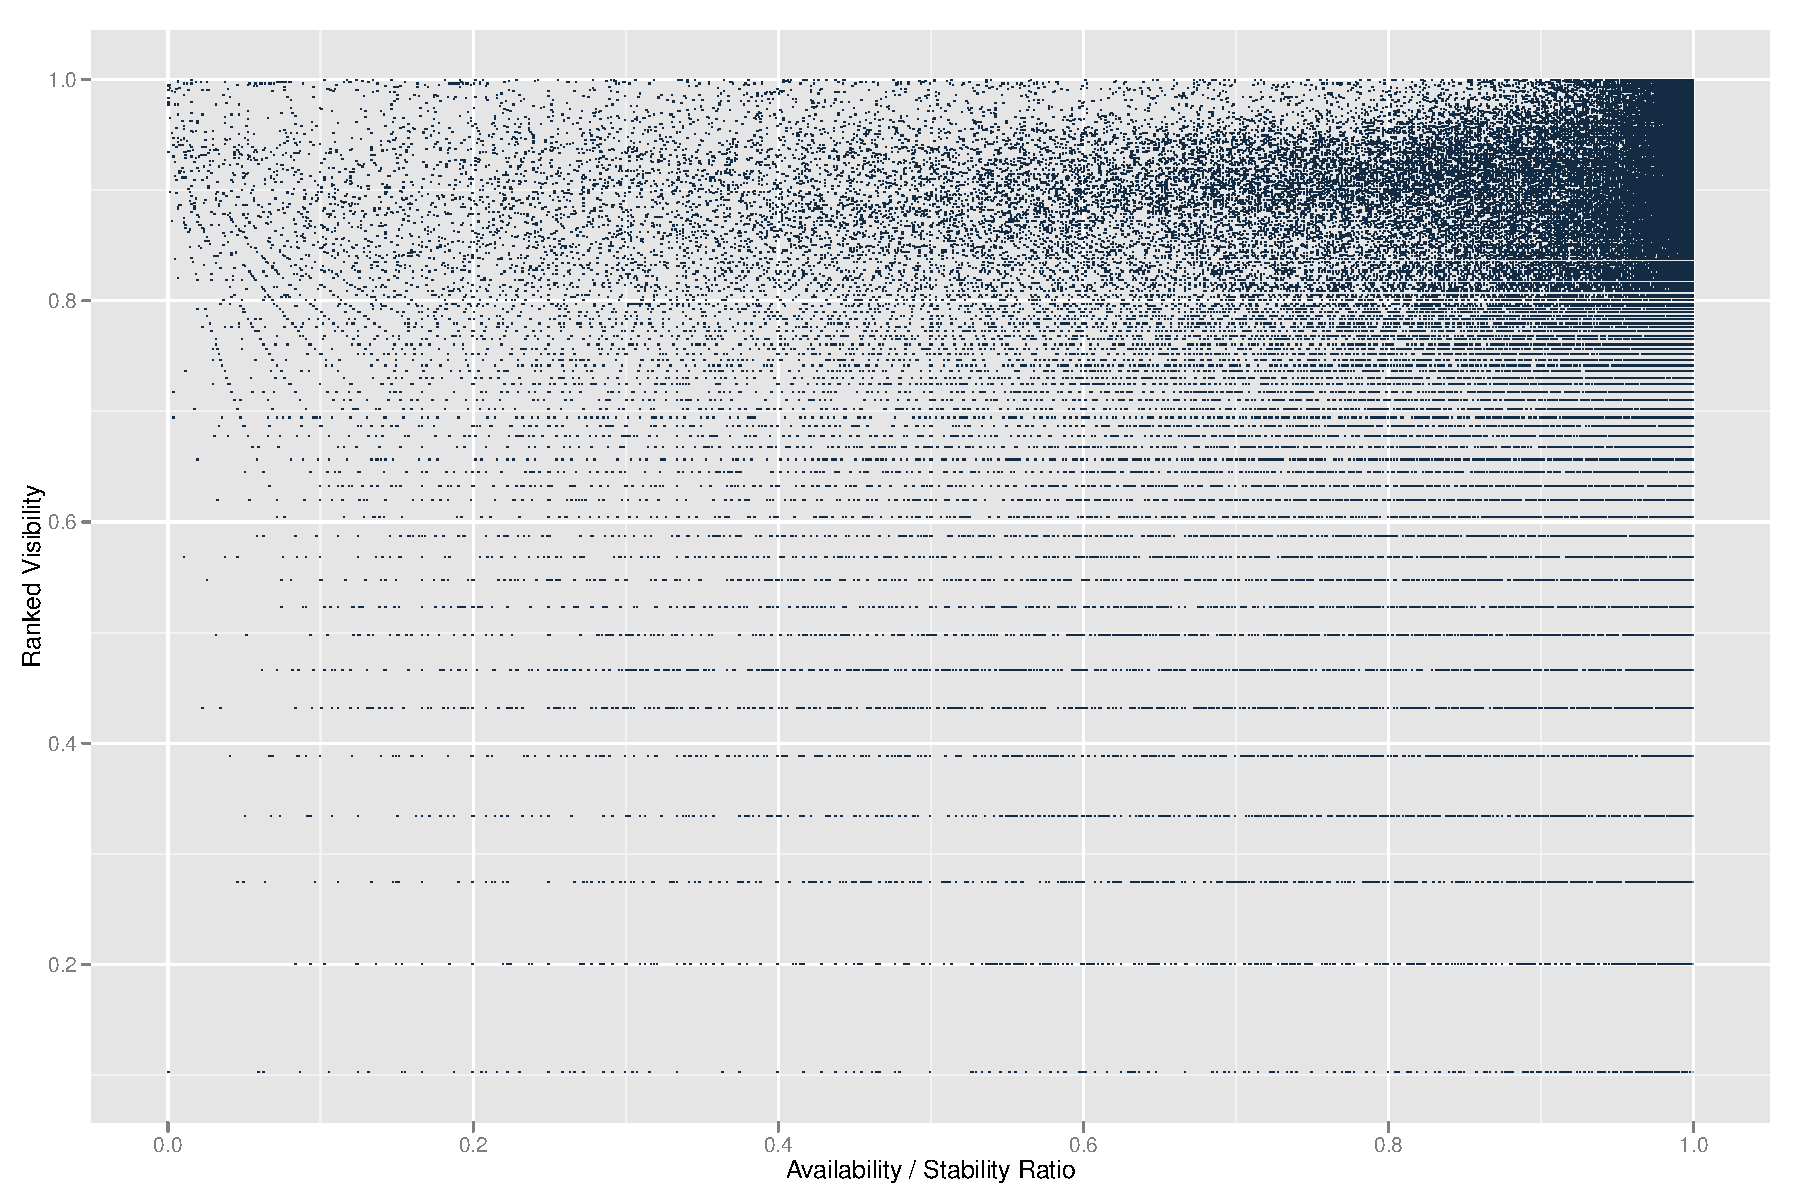
\includegraphics[width=\linewidth]{images/visibiliy_stability_map.pdf} \caption{Quantiles of the visible time slots of each socket and the corresponding stability stability} 
	\label{fig:rankedVisibility} 
\end{figure}

Furthermore, figures \ref{fig:ccdf_ratio_days} and \ref{fig:ccdf_ratio_vts} show each a complementary cumulated distribution function of the stability of server sockets with different visibilities.

One the one side, figure \ref{fig:ccdf_ratio_days} is using the daily visibility of the sockets. 
The red curve represents the distribution of the sockets which are seen only in one day. 
Not surprisingly, these group of \glspl{server socket} reveal the highest share of sockets with a stability of 1. 
This is mainly due to the fact that there is a high number of \glspl{server socket} which are active only during a relatively short period of time. This can be justified by looking at figure \ref{fig:vts_by_visibledays}.

Not surprisingly there is a higher share of sockets with a visibility of 2 days with a stability ratio below 80\%. 
Intuitively, the sockets which have a good visibility of 5 or even 6 days tend to have a high stability as well, but they have a lower share of sockets which have a stability ratio of 1 than all other. 
This means that sockets which are often visible incline to have at least some unbalanced connections.

On the other side, figure \ref{fig:ccdf_ratio_vts} shows the complementary cumulative distribution function of the stability ratio of sockets with different absolute visible time slots. 
Around 99\% of all \glspl{server socket} with more than 1000 visible time slots have a higher stability ratio than 95\%. 
Although, only around 20\% of them have a stability ratio of 100\%, i.e., they have no unbalanced connections at all. 
Thus, server sockets which are suitable for connectivity tracking must not have a stability of exactly 1. 
According to figure \ref{fig:ccdf_ratio_days}, \glspl{server socket} with a low visibility incline to have a higher share of sockets with a stability ratio below 90\% than sockets more often visible.
Besides the average stability of a server socket, it can be interesting to consider the variance of the stability as well. 
A low variance indicates that the socket was stable over time despite having some unidirectional connections, while a larger variance indicates some fluctuations over time. 
Therefore, the variance as metric for the momentum of the stability may considered as well for selecting stable sockets. 

\begin{landscape}
	\begin{figure}
		[p] \centering 
		\includegraphics[width=\linewidth]{images/CCDF_ratio_days.pdf} \caption{Complementary cumulative distribution function of the availability by visible days} 
		\label{fig:ccdf_ratio_days} 
	\end{figure}
\end{landscape}
\begin{landscape}
	\begin{figure}
		[p] \centering 
		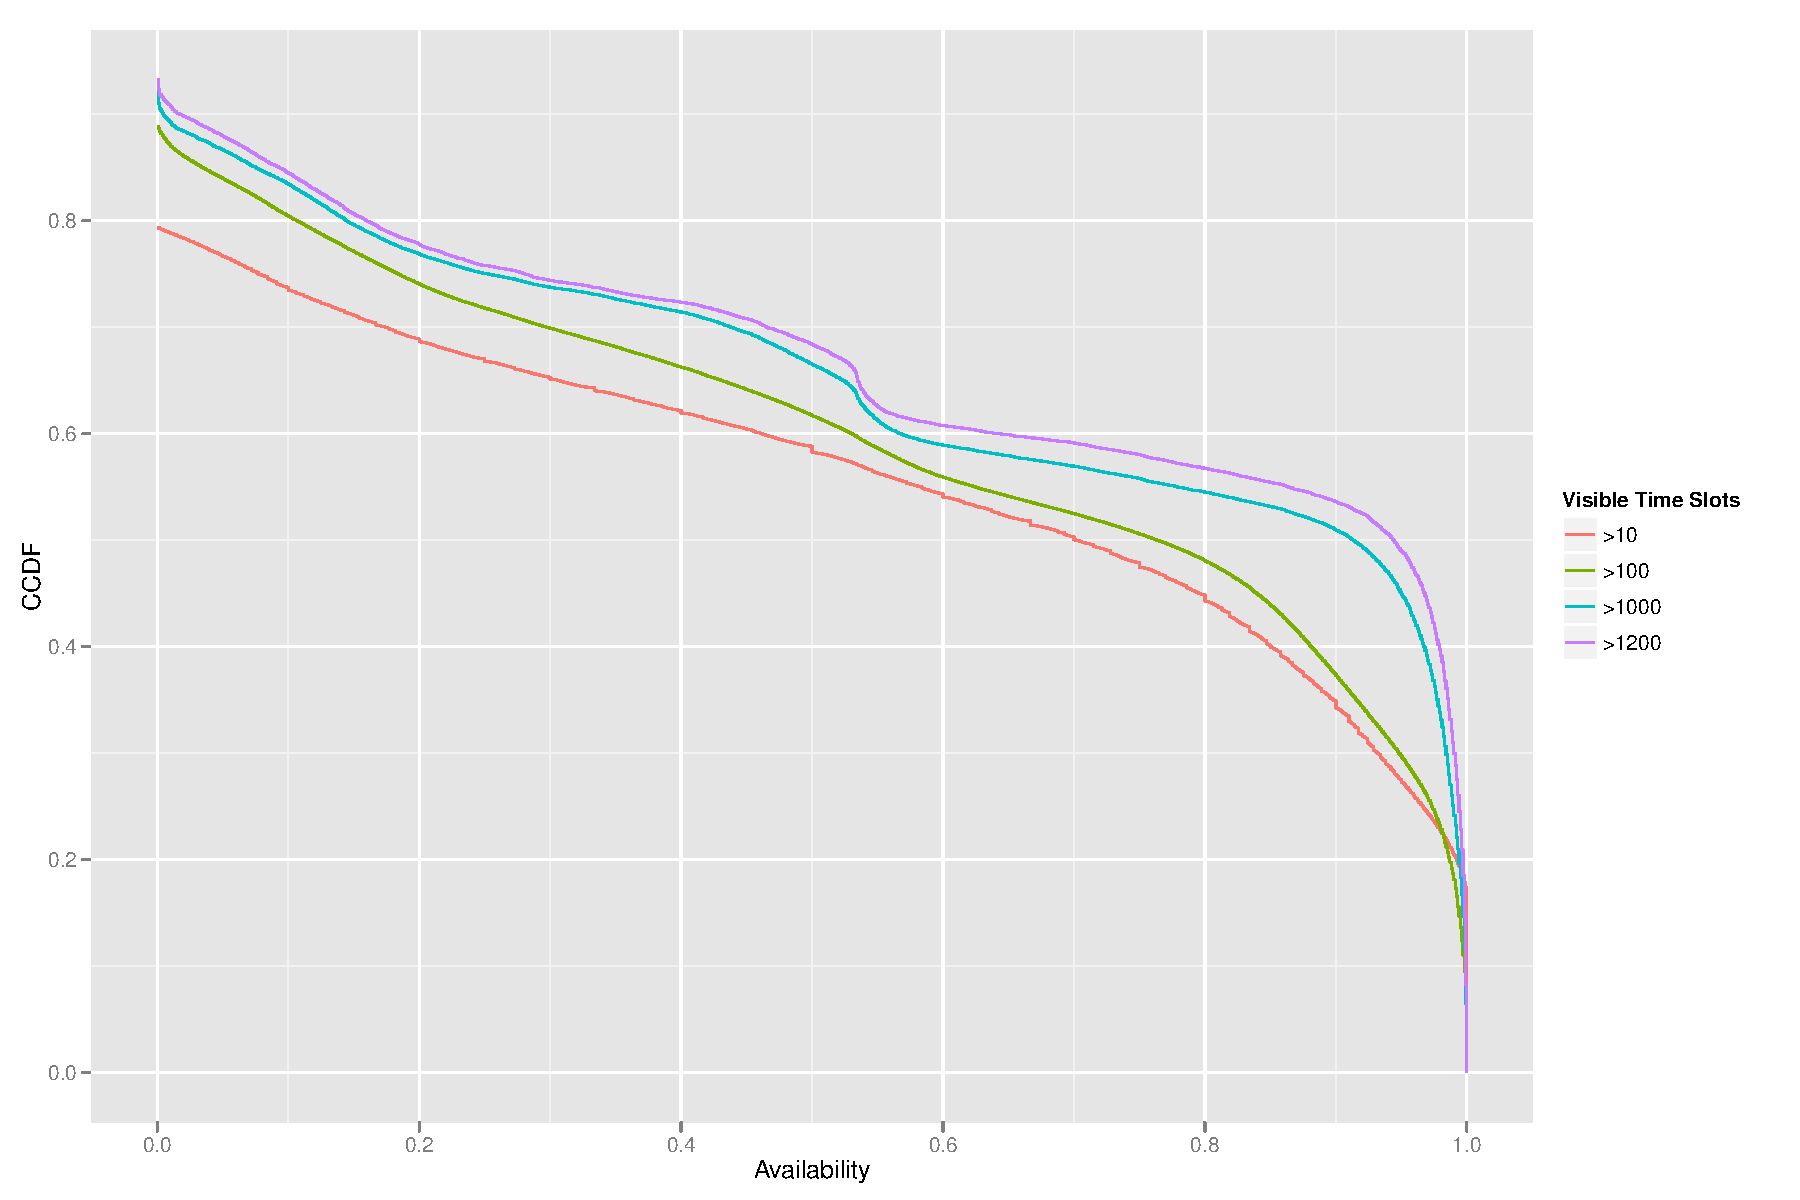
\includegraphics[width=\linewidth]{images/CCDF_ratio_VTS.pdf} \caption{Complementary cumulative distribution function of the availability by visible time slots} 
		\label{fig:ccdf_ratio_vts} 
	\end{figure}
\end{landscape}

\subsubsection{Popularity and Stability}

Similarly to the visibility, the \glspl{server socket} characteristics of popularity and stability are briefly assessed in the following. 
For this reason, figure \ref{fig:rankedPopularity} shows the \glspl{server socket} by their popularity quantiles and their stability. 
Hence, a \gls{server socket} with a popularity quantile of 80\% signifies that there are 80\% of all \gls{server socket} with a lower or equal popularity as this specific socket.

Similarly to figure \ref{fig:rankedVisibility}, the \glspl{server socket} tend to cluster in the top right corner of figure \ref{fig:rankedPopularity}. This indicates that popular sockets tend to have a good stability as well.
To this end, the popularity quantile is a good metric to reduce the number of sockets for selecting suitable server sockets for connectivity tracking, since there are enough popular sockets which are stable as well. 
\begin{figure}
	[ht] \centering 
	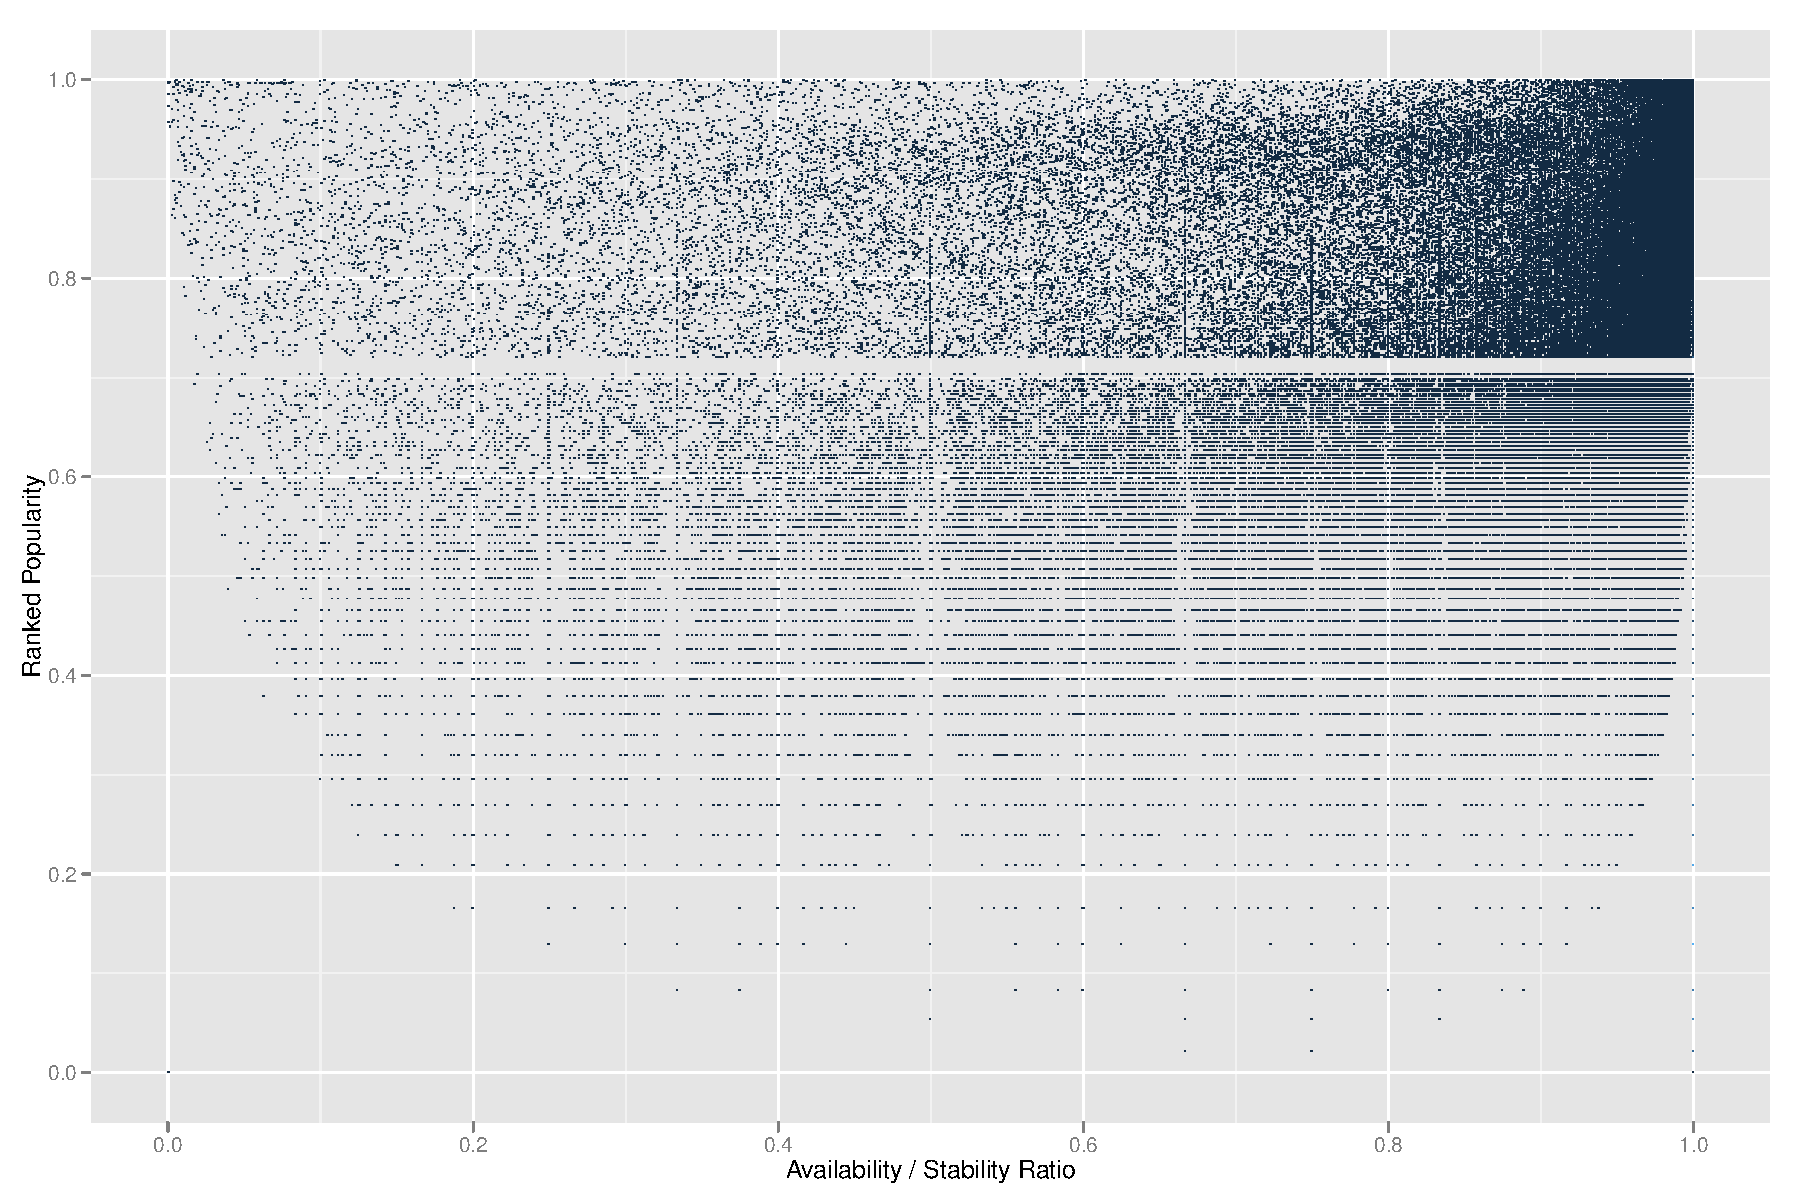
\includegraphics[width=\linewidth]{images/popularity_stability_map.pdf} \caption{Sockets by their ranked popularity and their stability} 
	\label{fig:rankedPopularity} 
\end{figure}

By aggregating all sockets by their protocol and port, some statistical insights can be gained, however, these insights are relative to a port centric view, since it does for example not differentiate the kind of application running on these sockets. 
Nonetheless, some useful information can be gained by comparing individual sockets with these port/protocol aggregated statistics of the same protocol and port. 
Hence, some statements about the characteristics relative to all other sockets can be made.

Table \ref{tab:top20_ports} shows the top 20 of all port and protocol aggregated sockets sorted by the total number of flows. Not surprisingly, UDP port 53 has the highest number flows during the observation period with around 46.68\% of all flows. 
However, in terms of sockets, UDP port 53 has only a share of 17.56\%. 
Not only with a total share of 32.32\% of all sockets, TCP port 80 is also with respect to number of flows dominating after UDP port 53. Furthermore, table \ref{tab:top20_ports} shows also some surprising results from the aggregation. 
%For example, there are 11 distinct sockets running on TCP port 555 which attract the almost 0.5\% of all flows. This is quite likely to be a result from malware, since port 555 is used by some trojans. 
It is interesting that also UDP port 123, officially assigned for \gls{NTP}, has a high number of flows, but only 318 external server sockets. Moreover, table \ref{tab:top20_ports} shows that the detection approach also manages to detect a high share of TCP high ports with a share of 37.21\% of all sockets and UDP high ports which are important with respect to the number of flows accounting for a share of 4.69\%.

\begin{table}
	[ht] \centering 
	\begin{tabular}{|c|r|r|r|r|r|r|} 
		\hline 
		\multirow{2}{*}{\textbf{Position}} & \multirow{2}{*}{\textbf{Port}} & \multirow{2}{*}{\textbf{Protocol}} & \multicolumn{2}{|c|}{\textbf{Flows}} & \multicolumn{2}{|c|}{\textbf{Sockets}} \\
		\cline{4-7} & & &absolute & relative & absolute & relative \\
		\hline \hline 1 & 53 & 17 & 1026787508 & 46.6799 & 327099 & 17.5634 \\
		\hline 2 & 80 & 6 & 845917736 & 38.4572 & 602008 & 32.3245 \\
		\hline 3 & 443 & 6 & 91197155 & 4.1460 & 67869 & 3.6442 \\
		\hline 4 & 555 & 6 & 10929909 & 0.4969 & 11 & 0.0006 \\
		\hline 5 & 22 & 6 & 10744151 & 0.4885 & 40797 & 2.1906 \\
		\hline 6 & 2703 & 6 & 10141483 & 0.4611 & 23 & 0.0012 \\
		\hline 7 & 25 & 6 & 9478055 & 0.4309 & 20155 & 1.0822 \\
		\hline 8 & 123 & 17 & 7119334 & 0.3237 & 318 & 0.0171 \\
		\hline 9 & 993 & 6 & 4377631 & 0.1990 & 1795 & 0.0964 \\
		\hline 10 & 12043 & 6 & 4002264 & 0.1820 & 294 & 0.0158 \\
		\hline 11 & 995 & 6 & 3157801 & 0.1436 & 962 & 0.0517 \\
		\hline 12 & 110 & 6 & 2808154& 0.1277 & 1662 & 0.0892 \\
		\hline 13 & 6005 & 6 & 2530274 & 0.1150 & 15 & 0.0008 \\
		\hline 14 & 53 & 6 & 2015993 & 0.0917 & 1467 & 0.0788 \\
		\hline 15 & 12200 & 6 & 1821843 & 0.0828 & 25 & 0.0013 \\
		\hline 16 & 3789 & 6 & 1796494 & 0.0817 & 10 & 0.0005 \\
		\hline 17 & 3478 & 17 & 1766902 & 0.0803 & 191 & 0.0103 \\
		\hline 18 & 2128 & 6 & 1694008 & 0.0770 & 390 & 0.0209 \\
		\hline 19 & 8080 & 6 & 1599711 & 0.0727 & 2269 & 0.1218 \\
		\hline 20 & 3128 & 6 & 1303533 & 0.0593 & 193 & 0.0104 \\
		\hline & other low & 6 & 4998962 & 0.2273 & 6705 & 0.3600 \\
		\hline & other low & 17 & 973753 & 0.0443 & 330 & 0.0177 \\
		\hline & other high & 6 & 49232031 & 2.2382 & 693126 & 37.2171 \\
		\hline & other high & 17 & 103241842 & 4.6936 & 94674 & 5.0835 \\
		\hline 
	\end{tabular}
	\caption{Top 20 port / protocol aggregated sockets by number flows} 
	\label{tab:top20_ports} 
\end{table}
Basically, figure \ref{fig:top20_ratio_box} shows a box-and-whisker plot of the stability of the 20 most popular ports. 
For most of the ports two box-plots are shown, one for \gls{UDP} in blue, and the other for \gls{TCP} in red. 
A box-and-whisker plot indicated with a box the range from the first quartile to the third quartile, also denoted as hinges, thus indicating where 50\% of all sockets of this kind are located. 
In the box, the median is illustrated by a black line. 
The whisker is connecting the hinges to the fences which represents the upper and lower extreme value. 
Moreover, some (statistical) outliners below or above the fences are shown by black dots.

Generally, it is important to see that there are indeed a high number of UDP sockets which are very stable. This is for example visible in figure \ref{fig:top20_ratio_box} for UDP 123, and UDP 53 which are both in the top 8 with respect to the number of flows.
On the other side, as for example TCP 6005 shows there are also TCP sockets which are very unstable and thus not suitable for connectivity tracking at all. 


Figure \ref{fig:top20_visibledays_box} shows number of visible days of the sockets in a box-and-whisker plot for the same top 20 port and protocol aggregated sockets. Remarkable are that an overwhelming share of UDP 123 sockets are visible on at least 4 days. Combining this insight with the insight on their stability most of the UDP 123 sockets may be very suitable for connectivity tracking. On the other side, almost all TCP port 22 sockets are visible only on a single day of the observation period. Hence, these TCP port 22 sockets are not suitable for connectivity tracking, despite the fact, that they are very stable as it can be seen in figure \ref{fig:top20_ratio_box}.

\todo{describe top 20 ports and reference table}



\begin{landscape}
	\begin{figure}
		[p] \centering 
		\includegraphics[width=\linewidth]{images/top20_ratio_box.pdf} \caption{box-and-whisker plot of the availability / stability of the top 20 traffic port server sockets} 
		\label{fig:top20_ratio_box} 
	\end{figure}
\end{landscape}
\begin{landscape}
	\begin{figure}
		[p] \centering 
		\includegraphics[width=\linewidth]{images/top20_visibility_box.pdf} \caption{box-and-whisker plot of visibility in days of the top 20 traffic port server sockets} 
		\label{fig:top20_visibledays_box} 
	\end{figure}
\end{landscape}

%%%%%%%%%%%%%%%%%%%%%%%%%%%%%%%%%%%%%%%%%%%%%%%%%%%%%%%%%%%%%%%%%%%%%%%%%%%%%%%%
% FACT EVALUATION
%%%%%%%%%%%%%%%%%%%%%%%%%%%%%%%%%%%%%%%%%%%%%%%%%%%%%%%%%%%%%%%%%%%%%%%%%%%%%%%%
\newpage
\section{Evaluation of Enhanced FACT\label{section:enhanced_FACT_eval}} 
In order to evaluate the effect of \gls{server socket} based traffic preselection, three known events were analyzed with the old port-based heuristic of \gls{FACT} as well as with the new \gls{server socket} based approach. 
Then, the results are compared and the effect of the traffic preselection on the noise of results is discussed qualitatively.

Three well known events are used in this evaluation and are already discussed in detail by \citet{SchatzmannPAM2011}. 
However, due to the lack of long enough data traces before each event which are required for detecting the \gls{server socket}, this evaluation relies on the detected \glspl{server socket} of data trace from the first week in November 2010. 
Nevertheless, from an operational point of view it seems that \glspl{server socket} from November are representative for the three events from March, May, and August as well.

For evaluating the \gls{server socket} based approach, several \glspl{server socket} sets are generated by restricting the number of sockets by imposing various conditions on their visibility, stability and popularity. 
By iteratively varying these conditions, different sets are generated and then, the overall IP space coverage as well as the total number of sockets of each set are determined. 
There were two starting sets for this iterative generation process. 
On the one side, all port 80 \glspl{server socket} formed the first initial set favoring a better comparison to the original port-based heuristic approach of FACT. 
On the other side, all detected \glspl{server socket} formed the second initial set to demonstrate that the approach is not limited to port 80 \glspl{server socket}. 

At first, all port 80 \glspl{server socket} are restricted by their stability and visibility in 10\% steps. Hence, there are 100 sets generated in total. 
For each set, the network coverage and the total size of \glspl{server socket} are determined. 

Because of the fact that the second initial set is containing three times the number of sockets compared to the first initial set.
The iterative generation process takes the popularity into account as well.
Again, the popularity is varied in 10\% steps as the visibility and stability. 
Hence, this set generation process generates 1000 different \glspl{server socket} sets and determines their IP space coverage and the number of sockets per set.

Since running \gls{FACT} for all three events is time and resource intensive, only 5 different sets are used with \gls{FACT} to evaluate their effects, so that \gls{FACT} is executed with all five sets on all three events. To compare the results from the socket based approach, \gls{FACT} is also executed with the old port-based heuristic approach. This results in 18 different executions of \gls{FACT}.

Table \ref{tab:ses_sets} provides a brief overview of the selected sets and the number of sockets contained in each set. 
As previously mentioned, to simplify the comparison of the new \gls{server socket} approach with the old heuristic port-based approach, three of the five selected sets are generated from the first initial set, thus only including port 80 \glspl{server socket}. In particular, set \emph{C} contains all external port 80 \glspl{server socket} and is the first initial set. 
By manual investigation of the evaluation of the generated port 80 sets, a visibility of 2 days and a stability of 90\% represented a good compromise between number of sockets and total network coverage. 
This set is denoted as set \emph{E}. To better understand the effect of the stability on \gls{FACT}, set \emph{D} contains only a condition on the visible days, thus allowing to compare set \emph{D} and \emph{E} for deducing the effect of imposing a stability condition. 
Furthermore, set \emph{A} is the second initial set, containing all detected \glspl{server socket}. 
Again, by manual investigation and comparing the IP space coverage and the number of sockets of a set, a last set is chosen with conditions imposed on visibility, stability and popularity. 
Set \emph{B} represented a good compromise between IP space coverage and number of sockets by requiring a popularity of 0.3. This means that the 70\% most popular sockets in term of flows are selected and then reduced by their visibility and stability. An additional constraint on the stability of set \emph{B} is that the variance of the stability of a socket have to be smaller than 0.1, therefore, the stability of the selected sockets is even more constrained than for set \emph{D} and \emph{E}.

Set \emph{A} consists of all detected \glspl{server socket}, Set \emph{B} is restricted to those socket with a ranked popularity of at least 30\%, a visibility of 2 days and a minimal stability ratio of 90\% and a maximal variance of the stability of 0.1. 
Hence, the set \emph{B} applies some limiting conditions on stability, visibility and popularity. 

Set \emph{C} contains all external port 80 \glspl{server socket}, allowing a direct comparison to the old port-based heuristic of \gls{FACT}. 
Furthermore, set \emph{D} reduces set \emph{C} to those sockets which are visible on more than 2 days. 
Finally, set \emph{E} is imposing an additional condition on the stability of sockets from set \emph{D}. 
\begin{table}
	[ht] \centering 
	\begin{tabular}
		{|c|c|c|c|c|c|} \hline \textbf{Socket Set} & \textbf{Ports} & \textbf{min. Stability} & \textbf{min. Visibility} & \textbf{min. Popularity} & \textbf{Sockets} \\
		\hline \hline A & all & 0 & 0 & 0 & 1862389 \\
		\hline B & all & 0.9\tablefootnote{additionally restricted to those sockets with a smaller variance of the stability than 0.1} & 2 days & 0.3 & 320531 \\
		\hline C & 80 & 0 & 0 & 0 & 602111 \\
		\hline D & 80 & 0 & 2 days & 0 & 418912 \\
		\hline E & 80 & 0.9 & 2 days & 0 & 384164\\
		\hline 
	\end{tabular}
	\caption{Overview of evaluated \gls{server socket} sets} 
	\label{tab:ses_sets} 
\end{table}

Table \ref{tab:ses_sets_coverage} shows the network coverage of each set with respect to their IP space coverage
\footnote{The covered IP space of FACT is calculated by the number of IP addresses of all prefixes containing at least one server socket of the set loaded into FACT}. 
The IP space is given in absolute terms and relative to the total IP space announced via BGP that week. Moreover, the IP space is also given in relative terms in reference to the maximum possible covered IP space of a server socket set, denoted as \emph{reference} in table  \ref{tab:ses_sets_coverage}.

As it can be seen in table \ref{tab:ses_sets_coverage}, \gls{FACT} is capable to observe almost 65\% of the announced IPv4 address space in November 2010. 
Contrasting this high observation scope of IPv4 address space, only a very small partition of the IPv6 address space is observable. 
A reason for this is, that the SWITCH backbone network was fully dual-stacked at that time, however, IPv6 traffic was in terms of flows almost negligible. Nonetheless, as IPv6 will continue to emerge in the next years, the IPv6 coverage will increase as well since the approach is not limited to IPv4 in any case. 

Besides that, it is also remarkable that set \emph{B} achieves a higher \gls{IPv4} space coverage than all port 80 socket sets despite having less sockets contained in this set and imposing harder criteria on popularity, and stability. 

\begin{table}
	[ht] \centering 
	\begin{tabular}
		{|c|c|r|r|r|r|r|} \hline \multirow{2}{*}{\textbf{Socket Set}} & \multicolumn{3}{|c|}{\textbf{IPv4 Space}} & \multicolumn{3}{|c|}{\textbf{IPv6 Space}} \\
		\cline{2-7} & absolute & reference & relative\tablefootnote{The announced IPv4 address space of all announced BGP prefixes is $2320427389$} & absolute & reference & relative\tablefootnote{The announced IPv6 address space of all announced BGP prefixes is $9.1196\cdot10^{33}$} \\
		\hline A & $1509368214$ & $100\%$ & $65.047\%$ & $3.7013\cdot10^{32}$ & $100\%$ & $4.059\%$ \\
		\hline B & $1060083001$ & $70.234\%$ & $45.685\%$ & $2.693\cdot10^{30}$ & $0.728\%$ & $0.030\%$ \\
		\hline C & $1027865637$ & $68.099\%$ & $44.296\%$  & $1.629\cdot10^{31}$ & $4.401\%$ & $0.179\%$ \\
		\hline D & $862625441$ & $57.151\%$ & $37.175\%$ & $1.408\cdot10^{31}$ & $3.804\%$ & $0.154\%$ \\
		\hline E & $831321169$ & $55.077\%$ & $35.826\%$ & $8.804\cdot10^{30}$ & $2.379\%$ & $0.097\%$ \\
		\hline 
	\end{tabular}
	\caption{Network coverage of the \gls{server socket} sets} 
	\label{tab:ses_sets_coverage} 
\end{table}

%%%%%%%%%%%%%%%%%%%%%%%%%%%%%%%%%%%%%%%%%%%%%%%%%%%%%%%%%%%%%%%%%%%%%%%%%%%%%%%%
% EVENT 1: AMS-IX PARTITIONING
%%%%%%%%%%%%%%%%%%%%%%%%%%%%%%%%%%%%%%%%%%%%%%%%%%%%%%%%%%%%%%%%%%%%%%%%%%%%%%%%
\subsection{Event 1: Partitioned Internet Exchange Point (IXP)}

The IXP \citet{AMS-IX}(AMS-IX) performed on March 23, 2010 a scheduled maintenance. 
When its connection to \citet{switch} came back, there was only a partial connectivity through this IXP, since some next-hops learned via their route servers were not properly reachable, thus traffic towards these networks was black-holed\citep{SchatzmannPAM2011}.

In consequence, several internal clients of the \citet{switch} network were complaining about unreachable external services on the next morning. 
Using classical debugging tools, it took more than four hours for fixing the problem by resetting a port\citep{SchatzmannPAM2011}.

\subsubsection{Heuristic Approach} This event is well visible by the classical \gls{FACT}, since there are quite a large number of affected users thus favoring the user aggregation approach of detecting relevant events. 
Figure \ref{fig:AMS_IX_FACT_REF} shows the number of unreachable \gls{bgp} prefixes over time separated by the number of affected internal clients. 
The user aggregation approach prioritizes severe events by determining the number of affected internal users. 
Hence, the severity of the events is indicated by the color of the unreachable prefixes in figure \ref{fig:AMS_IX_FACT_REF}. 
To be precise, the pink area visualizes the number of unreachable prefixes affecting at least 10 distinct internal clients, the blue area respectively at least 5 distinct internal clients.

This specific IXP partitioning event is clearly visible in figure \ref{fig:AMS_IX_FACT_REF} from 05.00 UTC to 08:15 UTC with almost 20 unreachable \gls{bgp} prefixes affecting more than 10 internal clients and almost 200 unreachable \gls{bgp} prefixes in total. 
However, as discussed in chapter \ref{Introduction}, those unreachable prefixes affecting only 1 or 2 clients are not reliable observations and are even representing a kind of observation noise. 
\begin{figure}
	[p] \centering 
	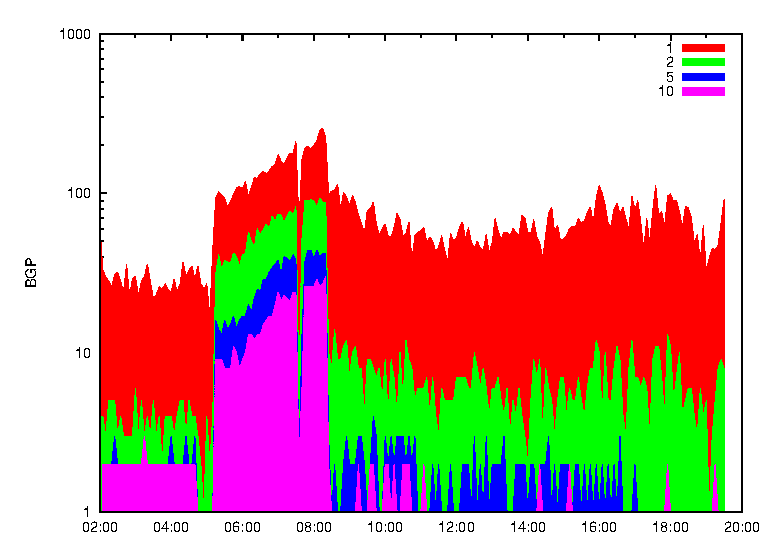
\includegraphics[width=0.75\linewidth]{images/events/2010_03_25/bgp_log_port80_ref.eps} \caption{Event 1: Unreachable \gls{bgp} prefixes detected by the classical \gls{FACT} traffic preselection based on the port-based heuristic.} 
	\label{fig:AMS_IX_FACT_REF} 
\end{figure}

\subsubsection{Server Socket Approach}

At first, \gls{FACT}'s results of set \emph{C} which contains all detected port 80 \glspl{server socket} are inspected. 
This socket set can directly be compared to the old heuristic approach, since it monitors a majority of the legitimate traffic to port 80 as well. 

As figure \ref{fig:AMS_IX_FACT_allSES80} shows, the actual event lasting from 05.00 UTC to 08:15 UTC is clearly visible equally well as in the heuristic approach from figure \ref{fig:AMS_IX_FACT_REF}. 
However, the \gls{server socket} based approach reduces the red part indicating the number of unreachable prefixes affecting only a single internal user by at least an order of magnitude. 
Hence, the event is now clearly standing out of the \emph{background event detection noise} -- the green and red part of figure \ref{fig:AMS_IX_FACT_REF}. 

Despite the fact that the set \emph{C} is not optimized at all with respect to stability, popularity and visibility, it outperforms the traditional approach in terms of noise reduction without significantly worsen the actual event detection. 
This confirms the assumption that a high number of unreachable prefixes affecting only a single internal user is caused by malware and \gls{p2p} churn.

Comparing the results from set \emph{C} to those from set \emph{D} which limits the sockets by only selecting the sockets seen at least at two days, yields almost no visual difference between figure \ref{fig:AMS_IX_FACT_allSES80VTS2} and \ref{fig:AMS_IX_FACT_allSES80}, despite the number of sockets is reduced by almost a third. 
However, if also the stability is considered as by set \emph{E}, the red and green noise can be further reduced without significantly affecting the blue and pink part of the event.

If the \glspl{server socket} are not anymore artificially constrained to be a port 80 \gls{server socket} as in the case of set \emph{A} and \emph{B}, there is a clear increase of unreachable sockets visible in figure \ref{fig:AMS_IX_FACT_allSES} with all server sockets and even in figure \ref{fig:AMS_IX_FACT_popularVTS2STAB9}. 
The original \gls{FACT} detects up to 30 unreachable prefixes with 10 or more internal users affected, \gls{FACT} with set \emph{A} and \emph{B} detect up to 112, respectively up to 72 distinct unreachable prefixes. 
Remarkable is that the red and green part of figure \ref{fig:AMS_IX_FACT_allSES} and \ref{fig:AMS_IX_FACT_popularVTS2STAB9} are significantly lower than in the case of the original results from figure \ref{fig:AMS_IX_FACT_REF} as well. 
\begin{figure}
	[p] \centering 
	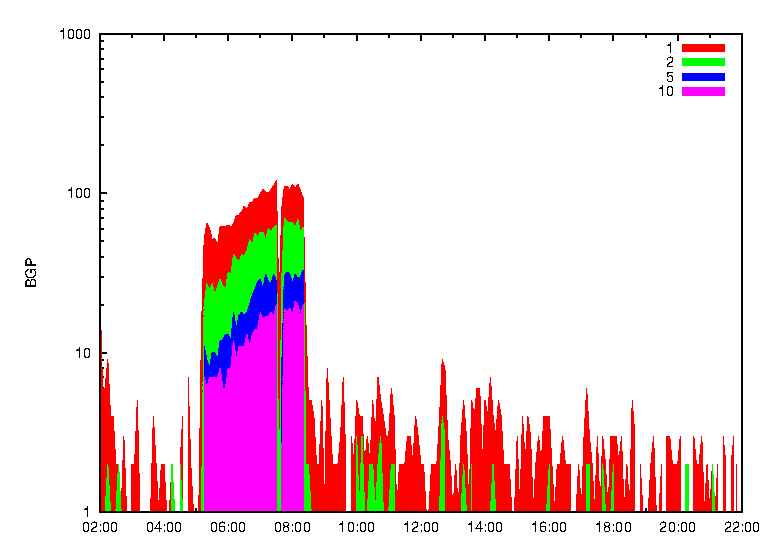
\includegraphics[width=0.75\linewidth]{images/events/2010_03_25/bgp_log_allPort80SES.eps} \caption{Event 1: Unreachable \gls{bgp} prefixes detected by the modified \gls{FACT} traffic preselection based on all port 80 \glspl{server socket}.} 
	\label{fig:AMS_IX_FACT_allSES80} 
\end{figure}
\begin{figure}
	[p] \centering 
	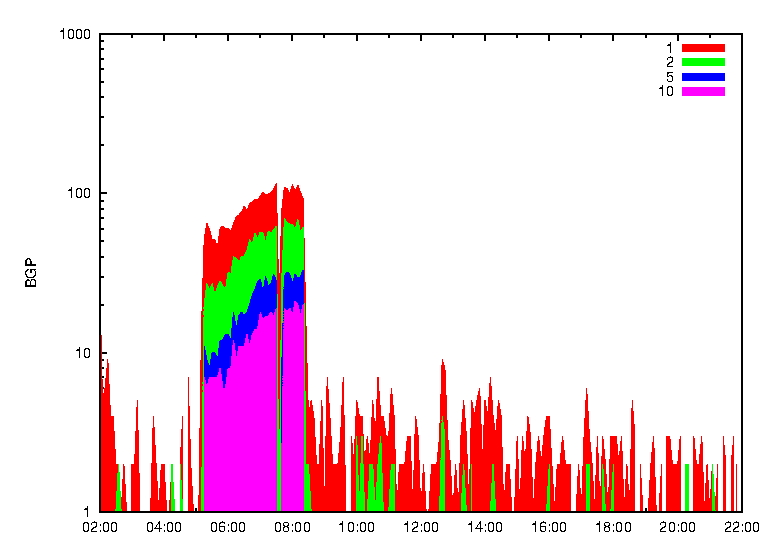
\includegraphics[width=0.75\linewidth]{images/events/2010_03_25/bgp_log_port80_Set_stab_0_vts_2.eps} \caption{Event 1: Unreachable \gls{bgp} prefixes detected by the modified \gls{FACT} traffic preselection based on all port 80 \glspl{server socket} with visibility of at least 2 days.} 
	\label{fig:AMS_IX_FACT_allSES80VTS2} 
\end{figure}
\begin{figure}
	[p] \centering 
	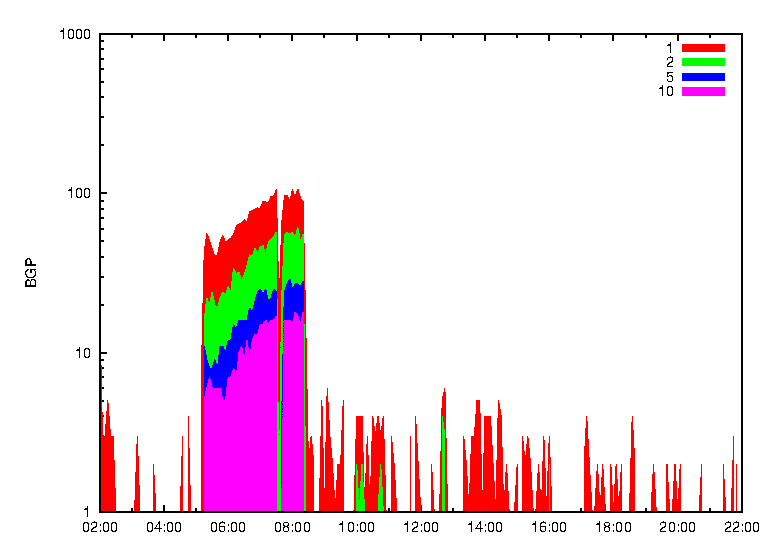
\includegraphics[width=0.75\linewidth]{images/events/2010_03_25/bgp_log_port80_Set_stab_9_vts_2.eps} \caption{Event 1: Unreachable \gls{bgp} prefixes detected by the modified \gls{FACT} traffic preselection based on all port 80 \glspl{server socket} with visibility of at least 2 days and stability ratio of at least $90\%$.} 
	\label{fig:AMS_IX_FACT_allSES80VTS2STAB9} 
\end{figure}
\begin{figure}
	[p] \centering 
	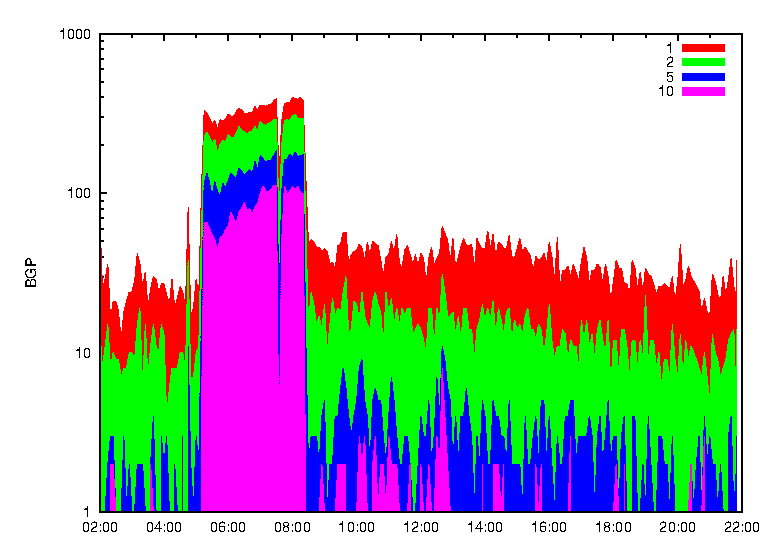
\includegraphics[width=0.75\linewidth]{images/events/2010_03_25/bgp_log_all_external.eps} \caption{Event 1: Unreachable \gls{bgp} prefixes detected by the modified \gls{FACT} traffic preselection based on all detected \glspl{server socket}} 
	\label{fig:AMS_IX_FACT_allSES} 
\end{figure}
\begin{figure}
	[p] \centering 
	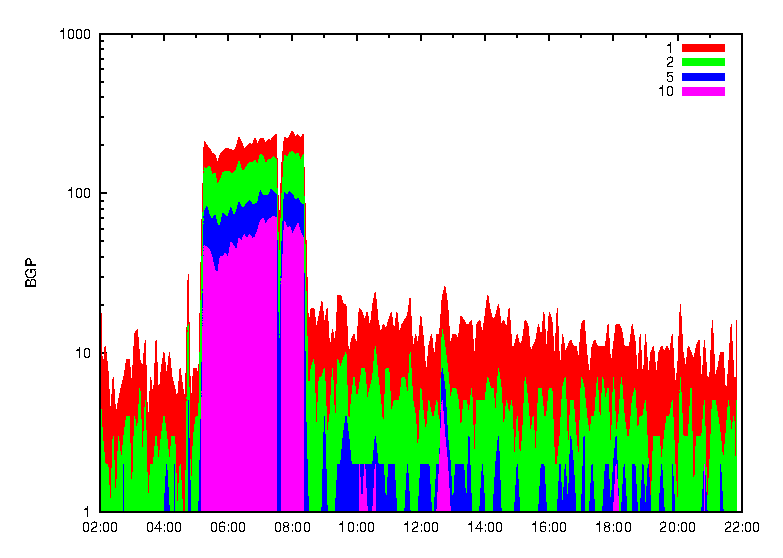
\includegraphics[width=0.75\linewidth]{images/events/2010_03_25/bgp_log_Set_var_0_1_stab_9_vts_2.eps} \caption{Event 1: Unreachable \gls{bgp} prefixes detected by the modified \gls{FACT} traffic preselection based on the $70\%$ most popular \glspl{server socket} limited to those with a visibility of at least 2 days and stability ratio of at least $90\%$.} 
	\label{fig:AMS_IX_FACT_popularVTS2STAB9} 
\end{figure}

%%%%%%%%%%%%%%%%%%%%%%%%%%%%%%%%%%%%%%%%%%%%%%%%%%%%%%%%%%%%%%%%%%%%%%%%%%%%%%%%
% EVENT 2: TIER-1 BLACK-HOLING
%%%%%%%%%%%%%%%%%%%%%%%%%%%%%%%%%%%%%%%%%%%%%%%%%%%%%%%%%%%%%%%%%%%%%%%%%%%%%%%%
\newpage 
\subsection{Event 2: Reverse Path Traffic Black-holing}

On May 18, 2010, the operators of the SWITCH network were assigned to investigate a reported issue that all services in an external /24 network were not accessible from the SWITCH network between 08:30 and 08:45 UTC. 
According to SWITCH, the problem was most likely due to an issue of an tier-1 provider which black-holed parts of the reverse traffic towards the SWITCH network\citep{SchatzmannPAM2011}.

Unfortunately, the operators were neither able to tell how many internal users were affected nor how many external networks were unreachable during this period of time. 
However with the help of \gls{FACT}, this issue can be further assessed with respect to the severity of the event\citep{SchatzmannPAM2011}.

\subsubsection{Heuristic Approach}

Figure \ref{fig:TIER1_FACT_REF} illustrates the unreachable prefixes detected by the port-based heuristic of \gls{FACT}. 
The event is indeed visible around 08:30 UTC until 08:45 UTC as a high pink peak. 
There are 12 external unreachable prefixes affecting more than 10 internal users. 
Furthermore, a strong diurnal pattern of the red and green area is visible in figure \ref{fig:TIER1_FACT_REF}. 
\begin{figure}
	[p] \centering 
	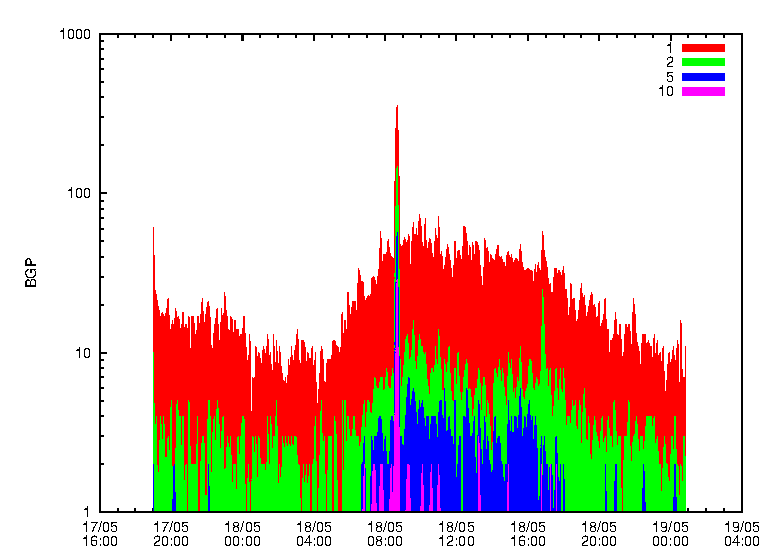
\includegraphics[width=0.75\linewidth]{images/events/2010_05_18/bgp_log_port80_ref.eps} \caption{Event 2: Unreachable \gls{bgp} prefixes detected by the classical \gls{FACT} traffic preselection based on the port-based heuristic.} 
	\label{fig:TIER1_FACT_REF} 
\end{figure}

\subsubsection{Server Socket Approach}

Again, the results of set \emph{C} which contains all port 80 \glspl{server socket} are directly comparable to the port-based heuristic approach. 
As figure \ref{fig:TIER1_FACT_allSES80} shows that the noise of the red and green area is reduced by at least an order of magnitude without worsen the real event detection at all.

Considering the visibility of the sockets as done by set \emph{D}, does not significantly change the visual appearance of the event at all as depicted by figure \ref{fig:TIER1_FACT_allSES80VTS2}. 
However, if the stability is considered as well by set \emph{E}, the noise can be even further reduced. 

By extending the set to all detected \glspl{server socket} (set \emph{A}), an increase of the unreachable prefixes by almost a factor of 6 is visible in figure \ref{fig:TIER1_FACT_allSES}. 
However, also the noise is increased, but still lower than the reference result from the port-based heuristic approach. 

By comparing figure \ref{fig:TIER1_FACT_allSES} with \ref{fig:TIER1_FACT_popularVTS2STAB9}, it becomes obvious that restricting the socket set by popularity, visibility and stability characteristics (set \emph{B}) does minimize the noise again by almost an order of magnitude with respect to all \glspl{server socket}. 
Additionally, it is remarkable that the diurnal pattern is less marked than in figure \ref{fig:TIER1_FACT_REF}. 
Though, no clear reason for this is identifiable. 
\begin{figure}
	[p] \centering 
	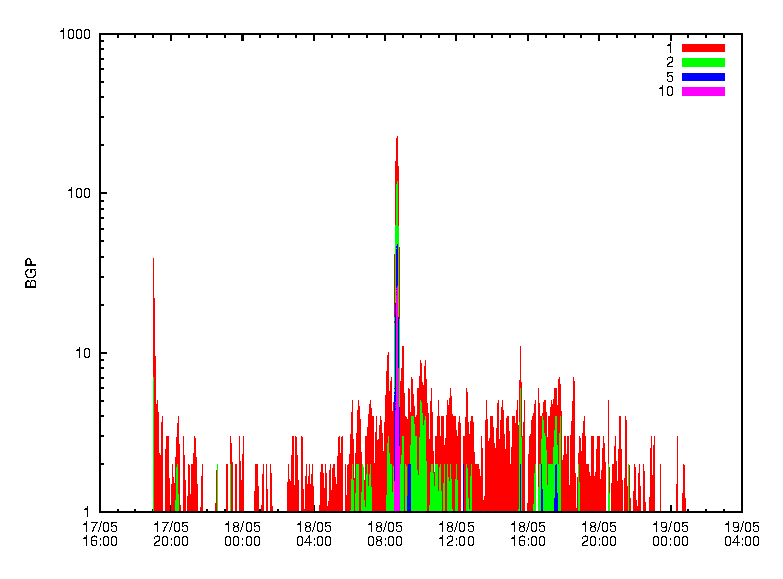
\includegraphics[width=0.75\linewidth]{images/events/2010_05_18/bgp_log_allPort80SES.eps} \caption{Event 2: Unreachable \gls{bgp} prefixes detected by the modified \gls{FACT} traffic preselection based on all port 80 \glspl{server socket}.} 
	\label{fig:TIER1_FACT_allSES80} 
\end{figure}
\begin{figure}
	[p] \centering 
	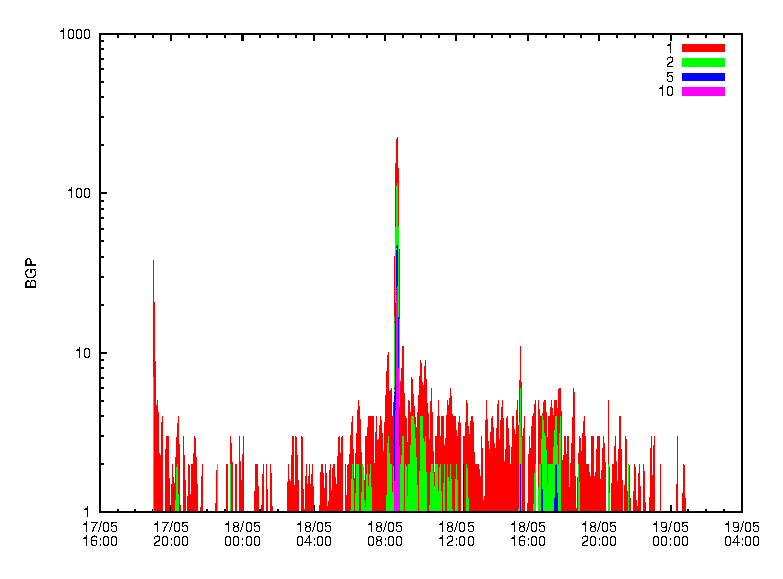
\includegraphics[width=0.75\linewidth]{images/events/2010_05_18/bgp_log_port80_Set_stab_0_vts_2.eps} \caption{Event 2: Unreachable \gls{bgp} prefixes detected by the modified \gls{FACT} traffic preselection based on all port 80 \glspl{server socket} with visibility of at least 2 days.} 
	\label{fig:TIER1_FACT_allSES80VTS2} 
\end{figure}
\begin{figure}
	[p] \centering 
	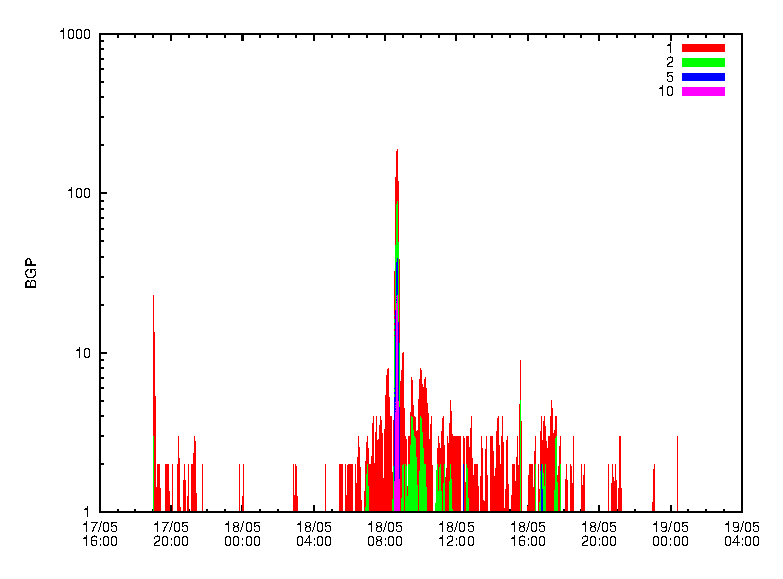
\includegraphics[width=0.75\linewidth]{images/events/2010_05_18/bgp_log_port80_Set_stab_9_vts_2.eps} \caption{Event 2: Unreachable \gls{bgp} prefixes detected by the modified \gls{FACT} traffic preselection based on all port 80 \glspl{server socket} with visibility of at least 2 days and stability ratio of at least $90\%$.} 
	\label{fig:TIER1_FACT_allSES80VTS2STAB9} 
\end{figure}
\begin{figure}
	[p] \centering 
	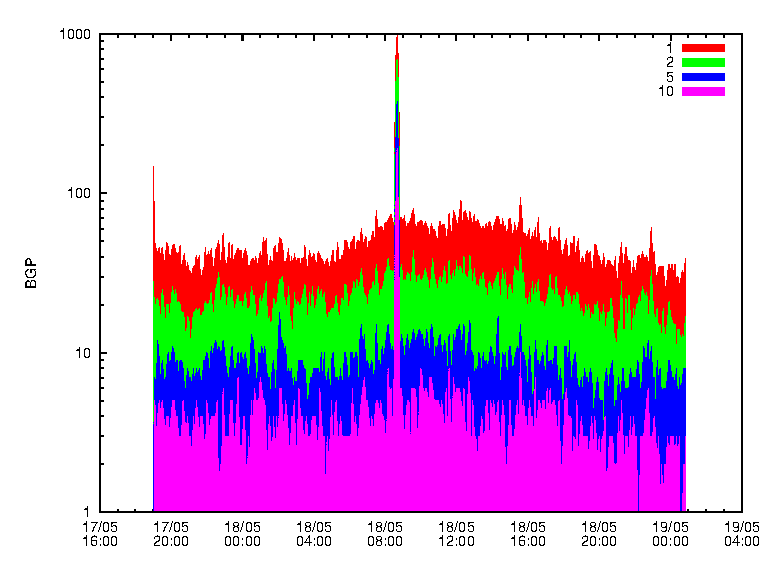
\includegraphics[width=0.75\linewidth]{images/events/2010_05_18/bgp_log_all_external.eps} \caption{Event 2: Unreachable \gls{bgp} prefixes detected by the modified \gls{FACT} traffic preselection based on all detected \glspl{server socket}} 
	\label{fig:TIER1_FACT_allSES} 
\end{figure}
\begin{figure}
	[p] \centering 
	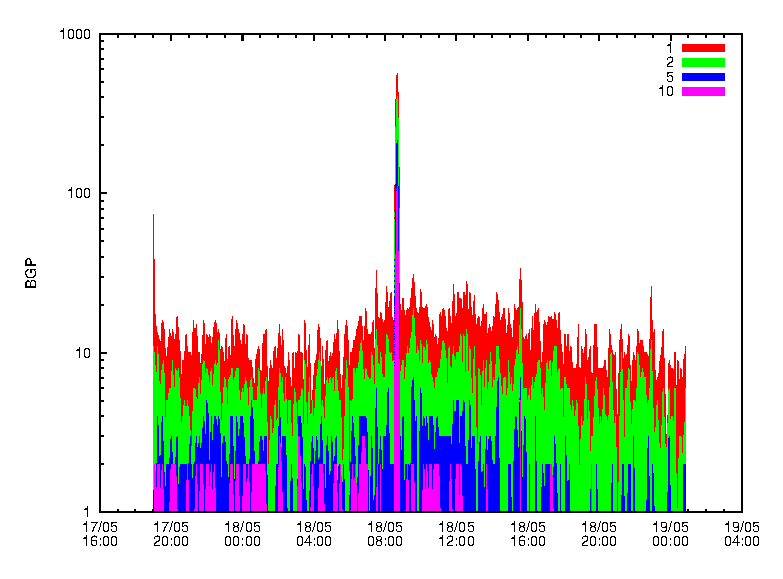
\includegraphics[width=0.75\linewidth]{images/events/2010_05_18/bgp_log_Set_var_0_1_stab_9_vts_2.eps} \caption{Event 2: Unreachable \gls{bgp} prefixes detected by the modified \gls{FACT} traffic preselection based on the $70\%$ most popular \glspl{server socket} limited to those with a visibility of at least 2 days and stability ratio of at least $90\%$.} 
	\label{fig:TIER1_FACT_popularVTS2STAB9} 
\end{figure}

%%%%%%%%%%%%%%%%%%%%%%%%%%%%%%%%%%%%%%%%%%%%%%%%%%%%%%%%%%%%%%%%%%%%%%%%%%%%%%%%
% EVENT 3: RIPE / DUKE BGP EXPERIMENT
%%%%%%%%%%%%%%%%%%%%%%%%%%%%%%%%%%%%%%%%%%%%%%%%%%%%%%%%%%%%%%%%%%%%%%%%%%%%%%%%
\newpage 
\subsection{Event 3: RIPE / DUKE BGP Experiments}

An experiment with new \gls{bgp} attributes jointly performed by RIPE and the Duke University on August 27, 2010, resulted in several unreachable prefixes\citep{SchatzmannPAM2011}. 
These new kind of attributes have never been announced on the Internet before, although the were in accordance with the \gls{bgp} specification\citep{ripe_duke}.

These new kind of attributes uncovered and triggered a bug in some Cisco router known as the \emph{Cisco IOS XR Software Border Gateway Protocol Vulnerability (SA-20100827-BGP)}\citep{cisco_vulnerability}. 
In particular, the announcements with the new attributes were corrupted by the Cisco routers and send to their peers. 
Consequently, their peers detected the corruption and dropped the entire peering session\citep{ripe_duke}.

\subsubsection{Heuristic Approach} 
Figure \ref{fig:RIPE_FACT_REF} shows the unreachable prefixes over time from August 26 2010 and August 27 2010. 
The RIPE / DUKE BGP experiment is visible in the results of \gls{FACT} from August 27 2010 08:50 UTC until 09:10 UTC with up to 3 unreachable prefixes affecting more than 10 internal users. 

The port-based heuristic approach of \gls{FACT} does report a high number of unreachable \gls{bgp} prefixes as unreachable affecting only one or two internal clients and showing a strong diurnal pattern thereof. 
\begin{figure}
	[p] \centering 
	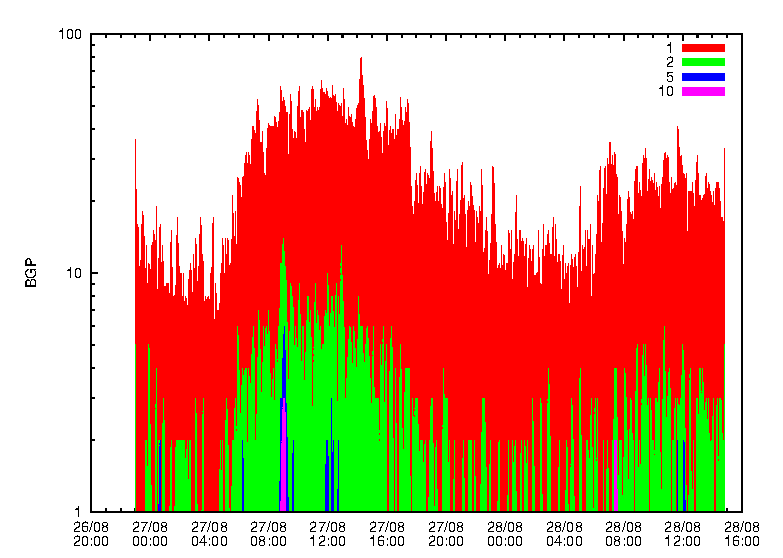
\includegraphics[width=0.75\linewidth]{images/events/2010_08_27/bgp_log_port80_ref.eps} \caption{Event 3: Unreachable \gls{bgp} prefixes detected by the classical \gls{FACT} traffic preselection based on the port-based heuristic.} 
	\label{fig:RIPE_FACT_REF} 
\end{figure}

\subsubsection{Server Socket Approach} 

By comparing figure \ref{fig:RIPE_FACT_REF} with figure \ref{fig:RIPE_FACT_allSES80} it becomes obvious that the \gls{server socket} based approach of figure \ref{fig:RIPE_FACT_allSES80} reduces the red and green area by an order of magnitude without restrain the visibility of the actual event shown in pink from 08:50 to 09:10 UTC. 
The adjusted traffic selection of \gls{FACT} yields exactly the same unreachable prefixes as the original port-based heuristic approach. 
Constraining set \emph{C} by the visible days of the sockets does not improve the noise reduction as figure \ref{fig:RIPE_FACT_allSES80VTS2} shows. 
However, the number of sockets of set \emph{D} is reduced by around a third compared to set \emph{C}, hence allowing a faster processing.

If as in case of set \emph{E} also the stability is considered, the noise is again reduced, although also at the cost of the event visibility. 
As figure \ref{fig:RIPE_FACT_allSES80VTS2STAB9} illustrates, \gls{FACT} detects only 2 unreachable prefixes affecting more than 10 internal users and hence, clearly missing one unreachable prefix. 

On the contrary, if \gls{FACT} is using set \emph{A}, it is able to reveal almost up to 20 unreachable prefixes affecting more than 10 internal users. 
Though, this comes at the cost of a even bigger red area than in case of the original port 80 based approach as it can be seen in figure \ref{fig:RIPE_FACT_allSES}. 
Luckily, as figure \ref{fig:RIPE_FACT_popularVTS2STAB9} shows \gls{FACT} is able to detect up to 14 distinct unreachable prefixes even with the smallest socket set. 
Moreover, the noise is considerably reduced compared to the port 80 based approach shown in figure \ref{fig:RIPE_FACT_REF}.
\begin{figure}
	[p] \centering 
	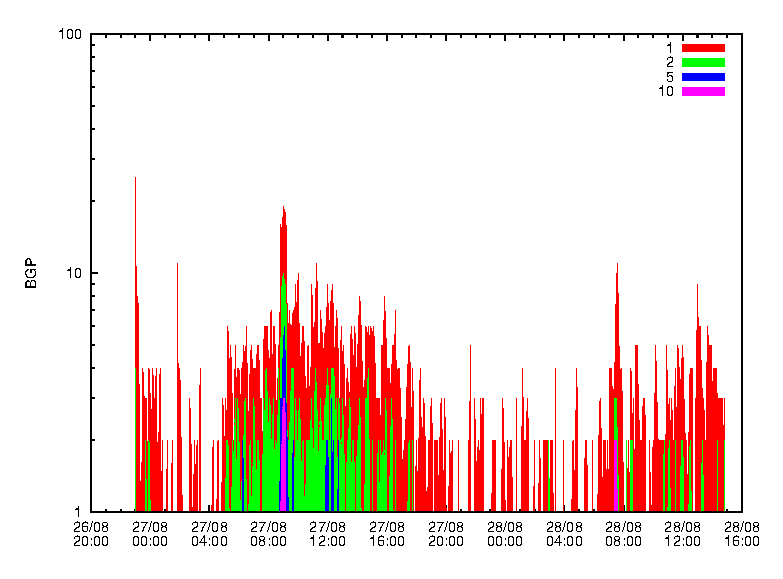
\includegraphics[width=0.75\linewidth]{images/events/2010_08_27/bgp_log_allPort80SES.eps} \caption{Event 3: Unreachable \gls{bgp} prefixes detected by the modified \gls{FACT} traffic preselection based on all port 80 \glspl{server socket}.} 
	\label{fig:RIPE_FACT_allSES80} 
\end{figure}
\begin{figure}
	[p] \centering 
	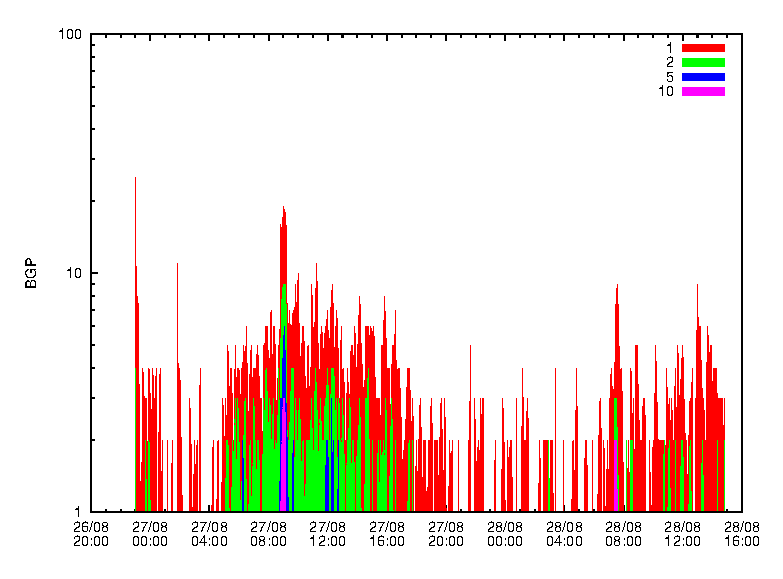
\includegraphics[width=0.75\linewidth]{images/events/2010_08_27/bgp_log_port80_Set_stab_0_vts_2.eps} \caption{Event 3: Unreachable \gls{bgp} prefixes detected by the modified \gls{FACT} traffic preselection based on all port 80 \glspl{server socket} with visibility of at least 2 days.} 
	\label{fig:RIPE_FACT_allSES80VTS2} 
\end{figure}
\begin{figure}
	[p] \centering 
	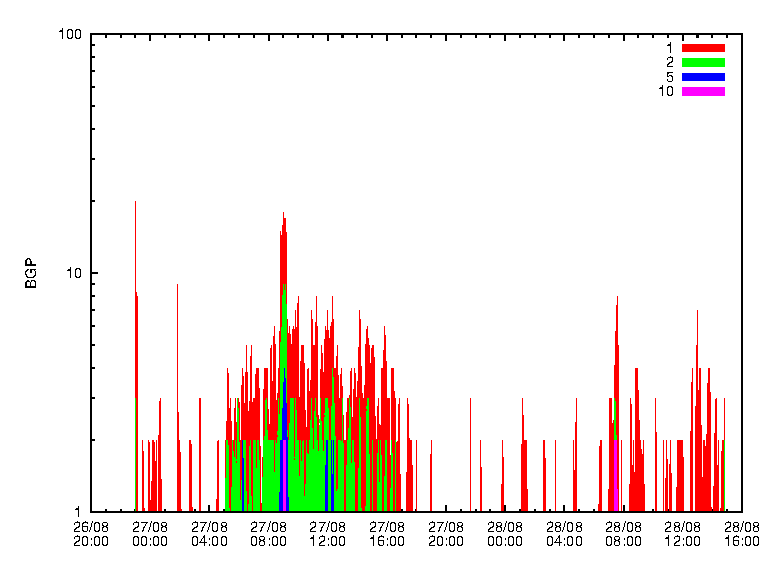
\includegraphics[width=0.75\linewidth]{images/events/2010_08_27/bgp_log_port80_Set_stab_9_vts_2.eps} \caption{Event 3: Unreachable \gls{bgp} prefixes detected by the modified \gls{FACT} traffic preselection based on all port 80 \glspl{server socket} with visibility of at least 2 days and stability ratio of at least $90\%$.} 
	\label{fig:RIPE_FACT_allSES80VTS2STAB9} 
\end{figure}
\begin{figure}
	[p] \centering 
	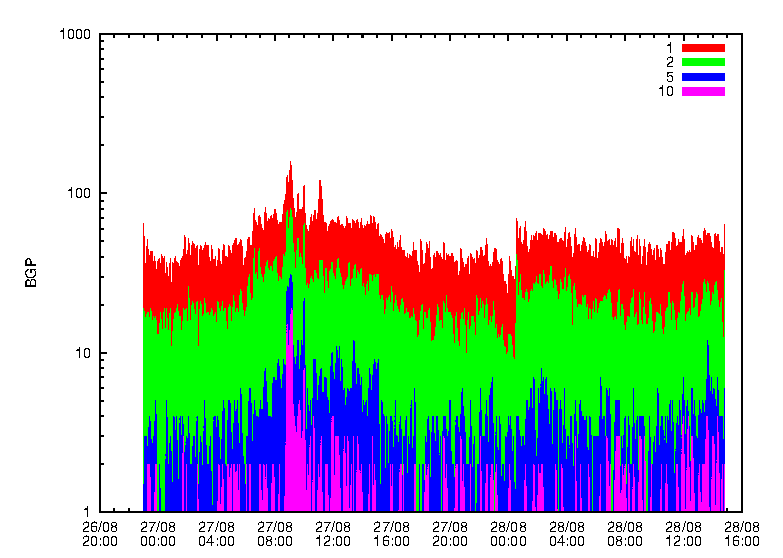
\includegraphics[width=0.75\linewidth]{images/events/2010_08_27/bgp_log_all_external.eps} \caption{Event 3: Unreachable \gls{bgp} prefixes detected by the modified \gls{FACT} traffic preselection based on all detected \glspl{server socket}} 
	\label{fig:RIPE_FACT_allSES} 
\end{figure}
\begin{figure}
	[p] \centering 
	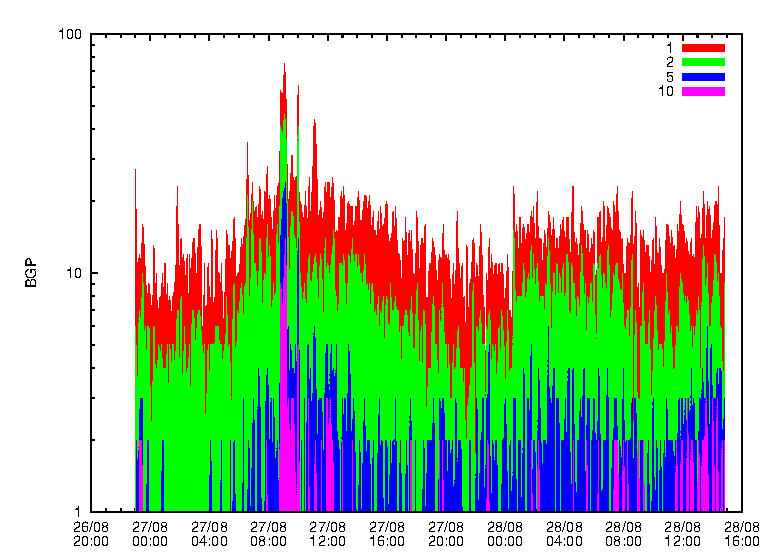
\includegraphics[width=0.75\linewidth]{images/events/2010_08_27/bgp_log_Set_var_0_1_stab_9_vts_2.eps} \caption{Event 3: Unreachable \gls{bgp} prefixes detected by the modified \gls{FACT} traffic preselection based on the $70\%$ most popular \glspl{server socket} limited to those with a visibility of at least 2 days and stability ratio of at least $90\%$.} 
	\label{fig:RIPE_FACT_popularVTS2STAB9} 
\end{figure}

%%%%%%%%%%%%%%%%%%%%%%%%%%%%%%%%%%%%%%%%%%%%%%%%%%%%%%%%%%%%%%%%%%%%%%%%%%%%%%%%
% RESULTS
%%%%%%%%%%%%%%%%%%%%%%%%%%%%%%%%%%%%%%%%%%%%%%%%%%%%%%%%%%%%%%%%%%%%%%%%%%%%%%%%
\newpage 
\section{Results\label{section:results}} 
Generally, \gls{FACT}'s results of the \gls{server socket} approach are better with almost all sets compared to the classic port-based heuristic. 
Though, there are significant differences between the results of the different \gls{server socket} sets. 

On the one side, constraining the sockets to be port 80 is good for comparing with the original approach, practically its too restrictive and as the comparison of the coverage from table \ref{tab:ses_sets_coverage} shows there is a better coverage with even less sockets possible. Hence, providing even a slightly better performance as well. 
Thus, it is possible to get either a greater network visibility as well as a more diverse observation space. Especially in case of the RIPE/DUKE event, this produces a much better view of the event. 

On the other side, constraining the sockets by their characteristics of visibility, stability and popularity allows to minimize the number of sockets by removing unsuitable sockets for connectivity tracking and thus, reducing the noise of the network outage event detection.

Sets set \emph{D} containts the least \glspl{server socket}, but provides a great visibility without generating to much noise.
Therefore, from the five evaluated sets, set \emph{D} is the best with respect to detection performance. 
However, as described previously the sets are chosen by manually comparing the network coverage and number of sockets, and thus, there may be other even better sets with respect to the detection performance. 
To find these sets the approach of selecting the sockets must be formally defined, e.g., as an optimization problem, and then adequately solved.

To sum up, the newly proposed approach of selecting the reflector traffic with the help of \glspl{server socket} actually decreases the detection noise and even provides a better event visibility and sensibility.
The performance of the approach is heavily influenced by the number of \glspl{server socket} which have to be considered during the generation of a good \gls{server socket} set.
Furthermore, this approach allows to better control the observation capabilities of \gls{FACT}, e.g., by completely excluding certain, uninteresting parts of the Internet from the observation scope.
%!TEX root = ./main.tex
\chapter{Conclusion\label{Conclusion}}

%\section{Conclusion}
Adjusting the traffic preselection of \gls{FACT} from a port-based heuristic to a \gls{server socket} based approach is far more than just a generalization. 

On the one hand, the \glspl{server socket} approach is less affected by scanning and \gls{p2p}, acting as a kind of history based scanning filter. 
Thus, reducing the negative effect of malware and \gls{p2p} churn on the network outage detection. 

On the other hand, a smart composition of the \gls{server socket} set used for the detection process may generally increase the observation coverage of \gls{FACT} without significantly increasing the noise ratio.
Hence, the practical usability of \gls{FACT} is increased even more.

The drawback of the approach is clearly that additional resources are required to store the \glspl{server socket} and the additional effort to detect, monitor and characterize the \glspl{server socket}. 
Nevertheless, the good results from chapter \ref{chapter:results} indicates that server sockets are quite stable over time and that there are even good results possible for events in March, May and August 2010 with sockets detected in 
November 2010. 

However, the selection of \glspl{server socket} can be cumbersome and directly influences the detection sensitivity of \gls{FACT}.
Though, even without any optimization the \gls{server socket} approach is clearly outperforming the original port-based heuristic with respect to the \emph{event-to-noise} ratio. 

\todo{Ausschmücken!! }

\newpage
\section{Future Work}
% characterize ses by time based activity (night / day, working week, weekend etc.)

In the future, new characterization methods can be investigated, especially the visibility allows to define different metrics, as day / night periods, working week activity or weekend activity.
These new metrics would allow to characterize a \gls{server socket} even more detailed.
Thus, getting a better view on the different properties of these sockets. 

% smarter socket set selection => density of network by choosing only the popularst sockets of each network
Furthermore, the \gls{server socket} set selection can be further enhanced by different techniques.
On the one hand, the density of \glspl{server socket} per prefix/network should be considered and examined.
By deducing the number of sockets required per network so that the probability of seeing traffic towards this network is maximized.
This would be clearly dependent on the single visibility of the selected sockets within this network.
Moreover, the general optimization problem can be mathematically expressed by defining an objective function.
This optimization problem may then be solved by different approaches as simulated annealing or integer linear programming.
In addition, the effect of the number of sockets of a set should be considered. 

% consider different selection methods as clustering analysis approaches, e.g. k-means etc => distance function include also network considerations.. etc. 
On the other hand, different selection approaches can be examined as well.
Given the problem scope of the socket selection based on different characteristics, clustering analysis approaches are worth to be considered. 

% automatization of process => danger of excluding sockets affected by events
% => consider full last week?  
Up to now, the process of detecting, monitoring and characterizing \glspl{server socket} is entirely independent from \gls{FACT}, therefore, an integration of these processing chains into \gls{FACT} should be considered. 
However, there is the danger of not selecting good sockets during potential events affecting these networks.
Hence, good approaches should not considering the (network) event periods during the characterizing phase of \glspl{server socket}.

% near future public release of FlowBox and FACT
Finally, the FlowBox library and the \gls{FACT} source code are intended to be released to public in the very near future, licensed under the GNU General Public License.


% Implementation
%%!TEX root = ./main.tex
\chapter{Background\label{Background}}

\section{FACT}


%

%!TEX root = ./main.tex
\chapter{Approach
\label{chapter:approach}}

\section{Methodology
\label{section:methodology}}

To achieve the goal of enhancing the traffic preselection of FACT with
knowledge about the past stability and popularity characteristics, the following
three steps are planned for extending FACT as illustrated in figure 
\ref{fig:FACT}.

\begin{figure}
	[ht] \centering
	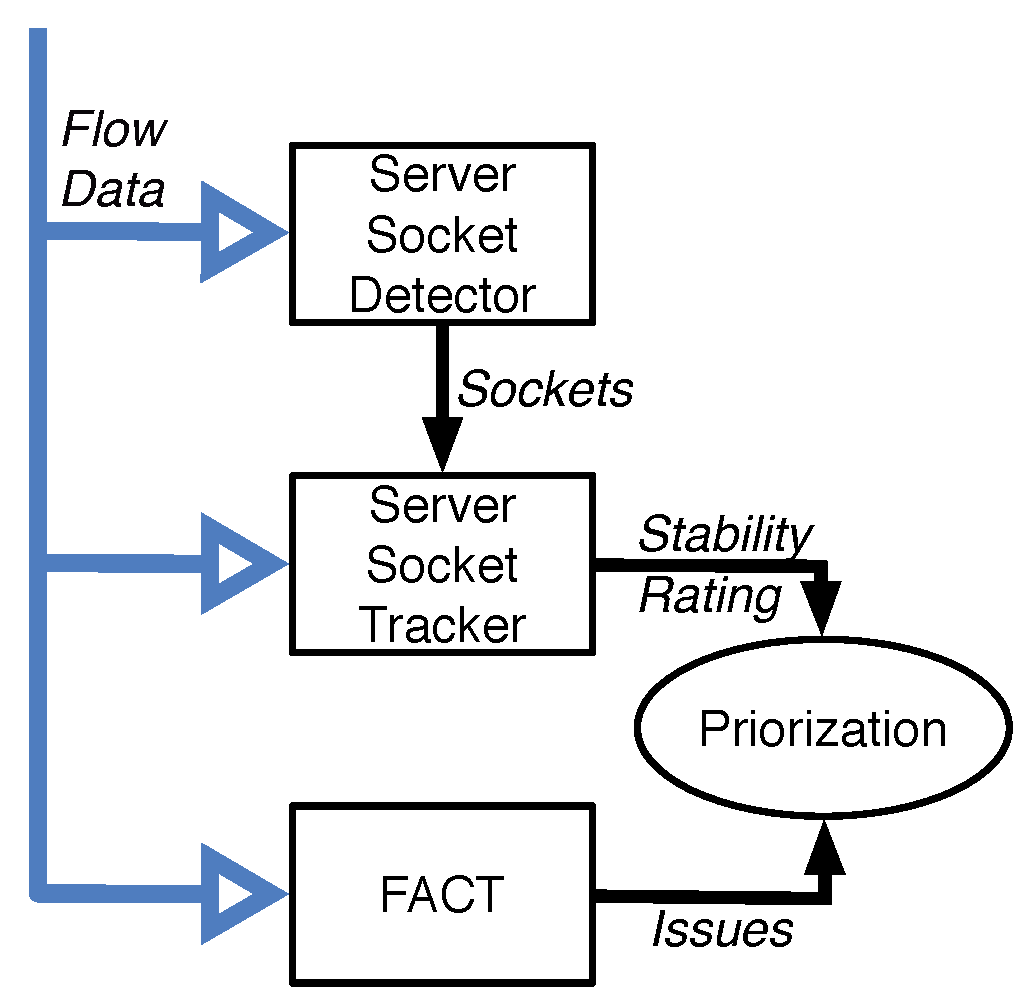
\includegraphics[width=8.5cm]{images/Approach_blockdiagram.eps}
	\caption{Interactions of new components with FACT} 
	\label{fig:FACT} 
\end{figure}

In a first step, a server socket detector is implemented. The challenge of the
server socket detection lies in the fact that the netflow data does not provide
enough precise timing information to determine which flow is originated from the
client and thereof deducing the server's socket. Therefore, the server socket
detection is achieved by the assumption that server sockets act as concentrators
in the sense that several clients have connections to the identical server
socket and bases on the work shown in
\cite{Schatzmann:Dissection,Schatzmann:Mining,Schatzmann:Tracing} and is
discussed in more detail in section \ref{section:socket_detection}.

Secondly, the previously detected server sockets are continually monitored and
especially the successful and unsuccessful connection attempts are recorded by
the server socket tracker.
Furthermore, these information are used to update the statistical information of
visibility, popularity and stability. Section \ref{section:socket_tracking}
covers this step in detail.

In a third step, the number of server sockets have to be reduced by selecting a 
set of suitable server sockets such that FACT is able to use these sockets for 
outage tracking. In particular, the server socket sets coverage of the Internet 
address space has to be assessed, because it makes for example no sense to 
select only the most popular sockets if they are all located in the same /24 
network which is discussed in more detail in section \ref{section:ses_selection}. Consequently, FACT has to be adopted to optimally use the preselected 
and rated server sockets for prioritizing relevant connectivity issues by 
reducing outage alerts based on single host outages of unstable services. This step is further discussed in chapter \ref{chapter:integration}.

%%%%%%%%%%%%%%%%%%%%%%%%%%%%%%%%%%%%%%%%%%%%%%%%%%%%%%%%%%%%%%%%%%%%%%%%%%%%%%%%
\section{Data
\label{section:data}}

This thesis relies on data collected at \citet{switch}, the Swiss National 
Research and Education Network (NREN). Mainly government institutions, 
universities, research labs are connected to the internet by \citet{switch}\citep{Schatzmann:Mining}.

The \citet{switch} network is with approximately 250'000 network users in 2010 comparable with a mid sized ISP. Currently, there are around 2.4 million IPv4 addresses, a /32 IPv6 and a /40 IPv6 network announced via BGP\citep{Schatzmann:Tracing}.

\begin{figure}[h] 
	\centering
	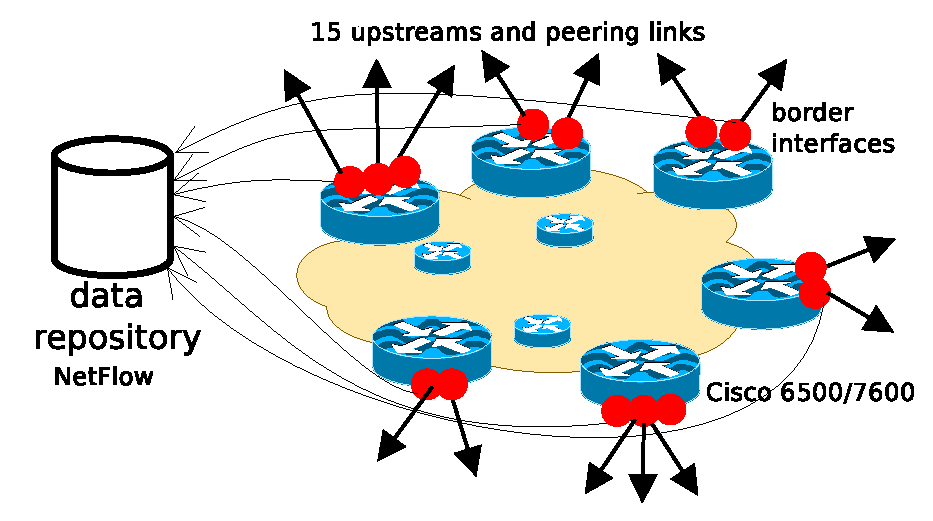
\includegraphics[width=12cm]{images/network_overview.eps}
	\caption{Overview of the SWITCH network \citep{SchatzmanThesis2012}} 
	\label{fig:switch_nework}
\end{figure}

Figure \ref{fig:switch_nework} is providing an overview of the SWITCH network. Currently, SWITCH has 15 upstreams and peering links and is capturing flow level data at all external interfaces of their border routers by 2003 in form of unsampled NetFlow data -- from 2003-2008 in version 5 and in version 9 after 2008\citep{Schatzmann:Tracing}.
High traffic peak rates of more than 80'000 flows per second, 3 million packets per second and more than 20Gbit/s require hardware-based flow collection cards. TCP flags are not available in the flow level information because of some limitations of these hardware components. The generated flow data is collected and stored at a central data repository.



% briefly describe the Switch network and its topology..
% traffic volume and netflow data unsampled!
% see tech report 338 for numbers and layout?! evtl actual numbers (2012)
%%%%%%%%%%%%%%%%%%%%%%%%%%%%%%%%%%%%%%%%%%%%%%%%%%%%%%%%%%%%%%%%%%%%%%%%%%%%%%%%
%

%!TEX root = ./main.tex
\chapter{Of Server Sockets and their Characteristics 
\label{chapter:sockets}}

\section{Server Sockets} Since the Internet has moved from a research project to a widely used, public communication infrastructure, one of the critical success factors was its diversity with respect to network applications or services. This was heavily favored by the Internets layered design as described by the OSI model. 

Todays network applications ranges from traditional services as web, FTP or mail to new and emerging services as video streaming and social networks. However, the term network application or service is overloaded and are differently used depending on the actual technical context.

Since this thesis will operate with flow-level data, layer 5-8 in the OSI model are invisible in the data set. Therefore, network services can be differentiated only by information based on layer 3 and 4 of the OSI model of the two connection end-points. For this reason, the following abstractions of a connection end-point are defined:

%%%%%%%%%%% SOCKET DEFINITION 			%%%%%%%%%%%%%%%%%%%%%%
\parbox{ 
\textwidth}{ 
\begin{defn}
	{\textbf{Socket}\\} A socket is uniquely defined by the triple (\textbf{IP address}, \textbf{IP protocol number} and \textbf{protocol port number}). A socket is only defined for IP protocol TCP(6) and UDP(17). 
\end{defn}
}

%%%%%%%%%%% SERVER SOCKET DEFINITION 	%%%%%%%%%%%%%%%%%%%%%%
\parbox{ 
\textwidth}{ 
\begin{defn}
	{\textbf{Server Socket 
	\label{def:serversocket}}\\} A server socket is a socket with a process listening to incoming connections and thus offering a network service. The lifetime of a server socket is not restricted to individual connections, but by the lifetime of the network service. 
\end{defn}
}

%%%%%%%%%%% CLIENT SOCKET DEFINITION 	%%%%%%%%%%%%%%%%%%%%%%
\parbox{ 
\textwidth}{ 
\begin{defn}
	{\textbf{Client Socket}\\} A client socket is a socket which is only used to initiate a connection to a server socket. Therefore, client sockets are of temporary lifetime which is limited by the duration this connection. 
\end{defn}
}

In spite of the containment of the term \emph{server} in definition \ref{def:serversocket}, this definition is not only valid for server-client application protocols, but also holds for P2P-applications. 
\todo{Explain more?}

\section{Detection of Server Sockets 
\label{section:socket_detection}}

% problem of detection with flow-level information (timing issue + flags)
Basically, a \emph{server socket} can be identified by the fact that a client opens a socket which initiates a connection to a \emph{server socket}. Usually, a \emph{client socket} is chosen at random by his operating system and the \emph{server socket} should be stable over time since it must offer a specific network service or application. Moreover, on each host a socket can only be assigned to one specific process per instance, i.e. a client socket connection initializing application or a \emph{server sockets} network application waiting on client connections. Otherwise, a socket-in-use-error is issued by the operating system. 

A straight-forward approach for detecting \emph{server sockets} is to infer the initiator of the connection by the timing information and determine its opposite as the \emph{server socket}. However, this approach requires a time synchronization of all flow exporting devices across the network. In practice, this can be hardly achieved in a satisfactory and reliable way.

% connection graph idea... +image
Hence, the detection of \emph{server sockets} with flow data relies on the following approach proposed by \citet{Schatzmann:Mining,Schatzmann:Dissection, Schatzmann:Tracing}. First of all, a communication graph is build as shown in figure \ref{fig:bipartite_graph}. This connection graph consists of nodes each representing an unique socket. If a bidirectional connection between two sockets is observed, an undirected, unweighted edge between the corresponding two nodes is assigned. This means that neither the direction nor the weight in terms of packets or bytes are required at all to build the connection graph. 
\begin{figure}
	[h] \centering 
	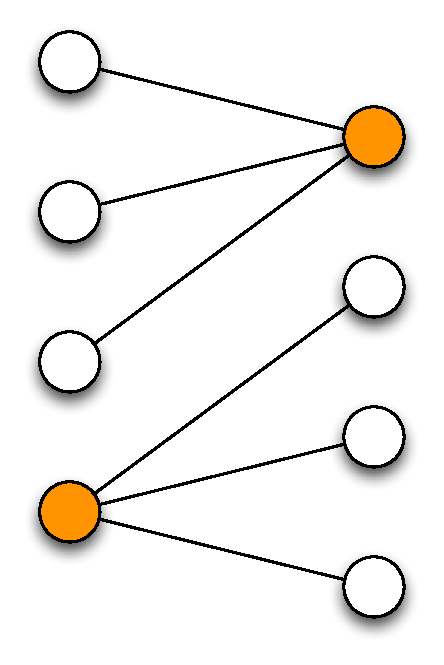
\includegraphics[width=\linewidth/3]{images/connection_graph.eps} \caption{Example of a bipartite connection graph with two concentrators of degree 3 marked as orange} 
	\label{fig:bipartite_graph} 
\end{figure}

In consequence of the fact that \emph{server sockets} provide a network application or service, they are likely to be contacted by several clients depending on their popularity. To this end, a socket which is contacted by a certain amount of client sockets and thus have a high degree in the connection graph is defined to be a \textbf{concentrator}. These concentrators are likely to offer a network service and are thus \emph{server sockets}. 
This approach is able to detect \emph{server sockets} which are offering not only classical client-server services,such as web, FTP, SSH, etc., but also p2p applications such as Skype, Bit-torrent super-nodes, etc. 
Therefore, it can be assumed that nodes with a high degree correspond to a \emph{server sockets}.

% introduce minimal vertex cover problem
% greedy algorithm to solve mvcp
% recalling sockets for optimization
\begin{algorithm}[t!]
\caption{Detection of server sockets by \citet{Schatzmann:Mining,Schatzmann:Dissection, Schatzmann:Tracing}}
\label{alg:service_tracing_ss-detection}
\begin{algorithmic}
\STATE
\STATE compute list $SS_{in}$ \COMMENT{int. sockets sorted by \# ext. clients}
\STATE compute list $SS_{out}$ \COMMENT{ext. sockets sorted by \# int. clients}
\STATE
\WHILE{(deg($SS_{out}[0]$) $ > 2 $ \OR deg($SS_{in}[0]$)$ > 2$)}
    \WHILE {(deg($SS_{in}[0]$) $ > $ deg($SS_{out}[0]$))}
        \STATE $ss$ = $SS_{in}[0]$ \COMMENT{classify $ss$ as internal server socket}
        \STATE remove $ss$ from $SS_{in}$
        \STATE update deg() for all entries of $SS_{in}$
    \ENDWHILE
    \WHILE{(deg($SS_{out}[0]$) $ \geq $ deg($SS_{in}[0]$))}
        \STATE $ss$ = $SS_{out}[0]$ \COMMENT{classify $ss$ as external server socket}
        \STATE remove $ss$ from $SS_{out}$
        \STATE update deg() for all entries of $SS_{out}$
    \ENDWHILE
\ENDWHILE
\end{algorithmic}
\end{algorithm}

% overall Algorithm of detection
\todo{detection approach chain!} 
\begin{figure}
	[ht] \centering \missingfigure{Detection Chain}
	
	%\includegraphics[width=\linewidth]{image/bipartite_graph.eps}
	\caption{Detection chain illustration} 
	\label{fig:detection_chain} 
\end{figure}

\section{Monitoring of Server Sockets 
\label{section:socket_tracking}}

The previous section outlined the approach of detecting \emph{server sockets}. This section covers the approach of monitoring flow data and generating statistical information such that some characteristics and properties of the found \emph{server sockets} can be assessed as outlined in section \ref{section:characterization}.

\subsection{Server Socket Statistics} The monitoring of the external \emph{server sockets} is done with help of the \emph{server socket registry} which is already used in the detection approach. This registry recalls all \emph{server sockets} which are known yet. Hence, all flows originated from a \emph{server socket} or flows which are destined for a \emph{server sockets} are monitored for compiling the socket statistics later used for the characterization.

In contrast to the detection approach, there are no scanning or other noise filters in the processing chain, because of the fact that they will remove at least some flows, mainly unidirectional flows, which are actually relevant for the statistics. 
\begin{figure}
	[ht] \centering \missingfigure{Monitoring Chain}
	
	%\includegraphics[width=\linewidth]{image/bipartite_graph.eps}
	\caption{Monitoring chain illustration} 
	\label{fig:monitoring_chain} 
\end{figure}

Since the processing is based on data containing flows which are active within a certain time slot, the statistics are accounted on a the same discrete time scale, i.e. 10 minutes. 
At first, each flow is checked if it is a flow of a \emph{server socket}. If this is the case, the individual flow statistics are accounted to the corresponding specific server socket \textbf{statistics record}. This includes the following entries: 
\vbox{

%
\begin{itemize}
	\item Number of bidirectional connections 
	\item Number of outgoing unidirectional connections 
	\item Number of incoming unidirectional connections 
\end{itemize}
}

In second step, the statistics records of each discrete time slot are aggregated in such a way that the information of the activity within a certain time slot is kept. Thus, the overall server socket statistics record contains the following entries: 
\vbox{

%
\begin{itemize}
	\item Sum of bidirectional connections of each time slot 
	\item Sum of outgoing unidirectional connections of each time slot 
	\item Sum of incoming unidirectional connections of each time slot 
	\item Number of days with connections 
	\item Number of discrete time slots with connections 
	\item Timestamps of discrete time slots with connections 
\end{itemize}
}

\subsection{Traffic Statistics} Besides of the individual server socket statistics report, overall traffic statistics are accounted, mainly for deducing knowledge of how good the monitoring capability of the server sockets in the registry is. For this reason, each flow which belongs to a server socket which is present in the registry is denoted as monitored. Hence, flows which does not belong to a server socket are accounted as not monitored. 

Moreover, all unmonitored flows can be further investigated for better understanding of the type of this unmonitored traffic. This can be done on the following three scopes: 
\vbox{

%
\begin{itemize}
	\item Protocol level 
	\item Port level for UDP and TCP flows 
	\item Direction 
	\item Type of connection 
\end{itemize}
}

The first scope, covers the problem that server sockets are only defined for protocol TCP and UDP, hence all flows with another protocol are per definition unmonitored.

Secondly, for all unmonitored TCP or UDP flows there is no corresponding server socket in the registry present. There are various reasons for this, mainly related to the detection approach outlined in section \ref{section:socket_detection}. In most of the cases, the sockets are not contacted by enough clients, therefore, the are not detected as concentrators and in consequence of that not denoted as server sockets. Furthermore, scanning activity is also a major contributor to this unmonitored flows, since scanning traffic and other non-legitimate traffic is removed before the server socket detection is performed. Consequently, these scanned sockets are not detected as server sockets, in case there is no legitimate traffic towards these sockets.

On the one hand, there is the possibility to account for each port the unmonitored flows which will lead to very detailed statistical information about the missed server sockets. However, this comes at the price of an inefficient processing and higher memory usage. 

On the other hand, the flows can be categorized by port ranges. In this thesis, there are just two ranges defined for this categorization:

\vbox{

%
\begin{itemize}
	\item Low port: 0-1024 
	\item High port: 1025-65365 
\end{itemize}
}

These categories are further divided by the location of the socket -- internal or external. Hence, the unmonitored TCP and UDP flows or strictly speaking the corresponding socket are accounted by the four categories:

\vbox{

%
\begin{itemize}
	\item external port high, internal port high 
	\item external port high, internal port low 
	\item external port low, internal port high 
	\item external port low, internal port low 
\end{itemize}
}

\section{Characterization of Server Sockets 
\label{section:characterization}} The main interest of this thesis is to characterize \emph{server sockets} by its \textbf{stability}, its \textbf{visibility} and its \textbf{popularity}. These properties tries to address the following characteristics of a server socket:

\vbox{ 
\begin{itemize}
	\item \textbf{Stability:} How stable is the \emph{server socket} regarding its responsiveness or availability: 
	\item \textbf{Visibility:} How frequently is the \emph{server socket} contacted by other socket: 
	\item \textbf{Popularity:} How many distinct sockets are contacting the \emph{server socket}: 
\end{itemize}
}

These three characteristics are directly deducible from the statistics observed by the passive monitoring technique outlined in \ref{section:socket_tracking}. In the following, each of the three characteristics are briefly discussed.

\subsection{Stability of a Server Socket} Because of the definition and its detection approach a \emph{server socket} is offering a bidirectional service which means that the client and the \emph{server socket} are both sending packets. Usually, a client socket is opening the connection to a \emph{server socket} which will reply in return to this request. Generally, this also holds for P2P applications as for example bit torrent. However in this case, there may be two \emph{server sockets} involved in the communication and no client socket. Therefore, a \emph{server socket} -- or the communication of it -- can be characterized as stable if all connections of this \emph{server socket} are \textbf{balanced}. 

%%%%%%%%%%% Balanced Connection DEFINITION 	%%%%%%%%%%%%%%%%%%%%%%
\parbox{ 
\textwidth}{ 
\begin{defn}
	{\textbf{Balanced Connection}\\} A connection between two sockets is balanced, if there is one flow originating from each socket which is destined for the other socket. Hence, the connection is bidirectional. 
\end{defn}
}

Thus, the overall stability \emph{server socket} or availability of its service can be approximated by the ratio of the balanced to all connections destined to this \emph{server socket}, i.e. the balanced and the unbalanced. This ratio is referred as a \emph{server socket} \textbf{stability ratio} and is mathematically defined by equation \ref{eq:ratio}. 
\begin{equation}
	\text{Stability}(\text{Socket}_i) = \frac{\text{balanced connections}(\text{Socket}_i)}{\text{balanced connections}(\text{Socket}_i) + \text{unbalanced connections}_{in}(\text{Socket}_i)} 
	\label{eq:ratio} 
\end{equation}

Hence, a \emph{server socket} with a stability ratio of 1 does only have bidirectional connections and thus, replies to all connection attempts. On the other side, a stability ratio of 0 indicates that there are only connections attempts by client sockets, but the server socket never replied upon these request. Unbalanced outgoing connections from the server sockets are indicating a client error or scanning activities of clients with spoofed (internal) source address which are not observed by the monitoring system. Therefore, these unbalanced outgoing connections are not considered for determining the stability ratio at all.

\subsection{Visibility of a Server Socket}

% discrete time slots activities of a socket, per day, per 5min slot?
% distribution is heavy-tailed, alot of sockets only rarely connected => due to scanning? due to malware?
The monitoring process of the server sockets is done passively, thus if a server socket is visible in the flow level data of a certain time period, the server socket is active during at that time. Hence, the visibility of a server socket during a certain time interval $t+\Delta{t}$ is a binary measure, either inactive in case it is not visible or active in case it is visible in the data set. Equation \ref{eq:visibility} defines the visibility of a socket during the time interval $t+\Delta{t}$: 
\begin{equation}
	\text{Visibility}_t(\text{Socket}_i,t+\Delta{t}) = \left\{ 
	\begin{array}{l l}
		1 & \quad \text{if $\text{Socket}_i$ is active during $t+\Delta{t}$}\\
		0 & \quad \text{if $\text{Socket}_i$ is not active during $t+\Delta{t}$}\\
	\end{array}
	\right. 
	\label{eq:visibility} 
\end{equation}

In consequence, there are different granularities $\Delta{t}$ to define the visibility a server socket. On the one hand, the most fine-grained resolution is just the flow-level data observation period. In most of the cases, this flow-level data observation period is set to 300 seconds. This fine-grained resolution is referred as the \emph{time slot} resolution, since the entire processing is based on such discrete time slotted data, containing all flows active during this time period. 
On the other hand, there are several other more coarse-grained resolutions of the visibility possible. The most obvious is a day long resolution, i.e. $\Delta{t} = 86400$s.

Furthermore, the visibility of a server socket can be extended from a single time period to the overall observation time, i.e. a week long trace, by summing up the individual visibilities of each time slot as shown in equation \ref{eq:visibility_sum}.
\begin{equation}
	\text{Visibility}(\text{Socket}_i) = \sum_{t} \text{Visibility}_t(\text{Socket}_i,t+\Delta{t})
	\label{eq:visibility_sum} 
\end{equation}

However, this summing approach exacerbate the comparison between different observations since it represents the visibility in absolute terms. Therefore, an even better metric for the visibility of a server socket is to average the individual $\text{Visibility}_t(\text{Socket}_i,t+\Delta{t})$ as outlined by equation \ref{eq:visibility_avg}. This normalizes the visibility to a value in the range between 0 and 1, representing the ratio of its visibility to the maximum visibility possible. Thus, a value of 1 means that the socket is visible in every single time slot and a value of 0 that the socket was never active. 
\begin{equation}
	\overline{\text{Visibility}}(\text{Socket}_i) = \frac{\sum_{t} \text{Visibility}_t(\text{Socket}_i,t+\Delta{t})}{\sum_{t}1}
	\label{eq:visibility_avg} 
\end{equation}

\subsection{Popularity of a Server Socket}

% number of flows / clients?.. degree of Server Socket
Besides the visibility of a server socket, its popularity is another major key characteristics. Whereas the visibility of a server socket defines how frequent in time a socket is contacted by at least one connection endpoint, the popularity of a server socket is defined by the number of connection attempts of client sockets during a certain period of time. The popularity of server socket can be deduced by various metrics as the number of flows, bytes or clients.

%% statistics
\newpage
\section{Analysis of Server Sockets in the Wild}

This section covers a detailed analysis of server socket found during a week long data trace from 2010/11/01 till 2010/11/05 -- the first 5 working days in November 2010.

\subsection{Detected Server Sockets}

% sum up of detection parameters > 2 biflows per 5min interval with more TCP packets > 3 UDP > 1

% state overall number of detected external and internal server sockets during this period

\subsection{Server Sockets Flows Gravity}
% traffic statistics of server sockets detected by type and ratio of traffic towards server sockets


\begin{figure}
	[ht] \centering 
	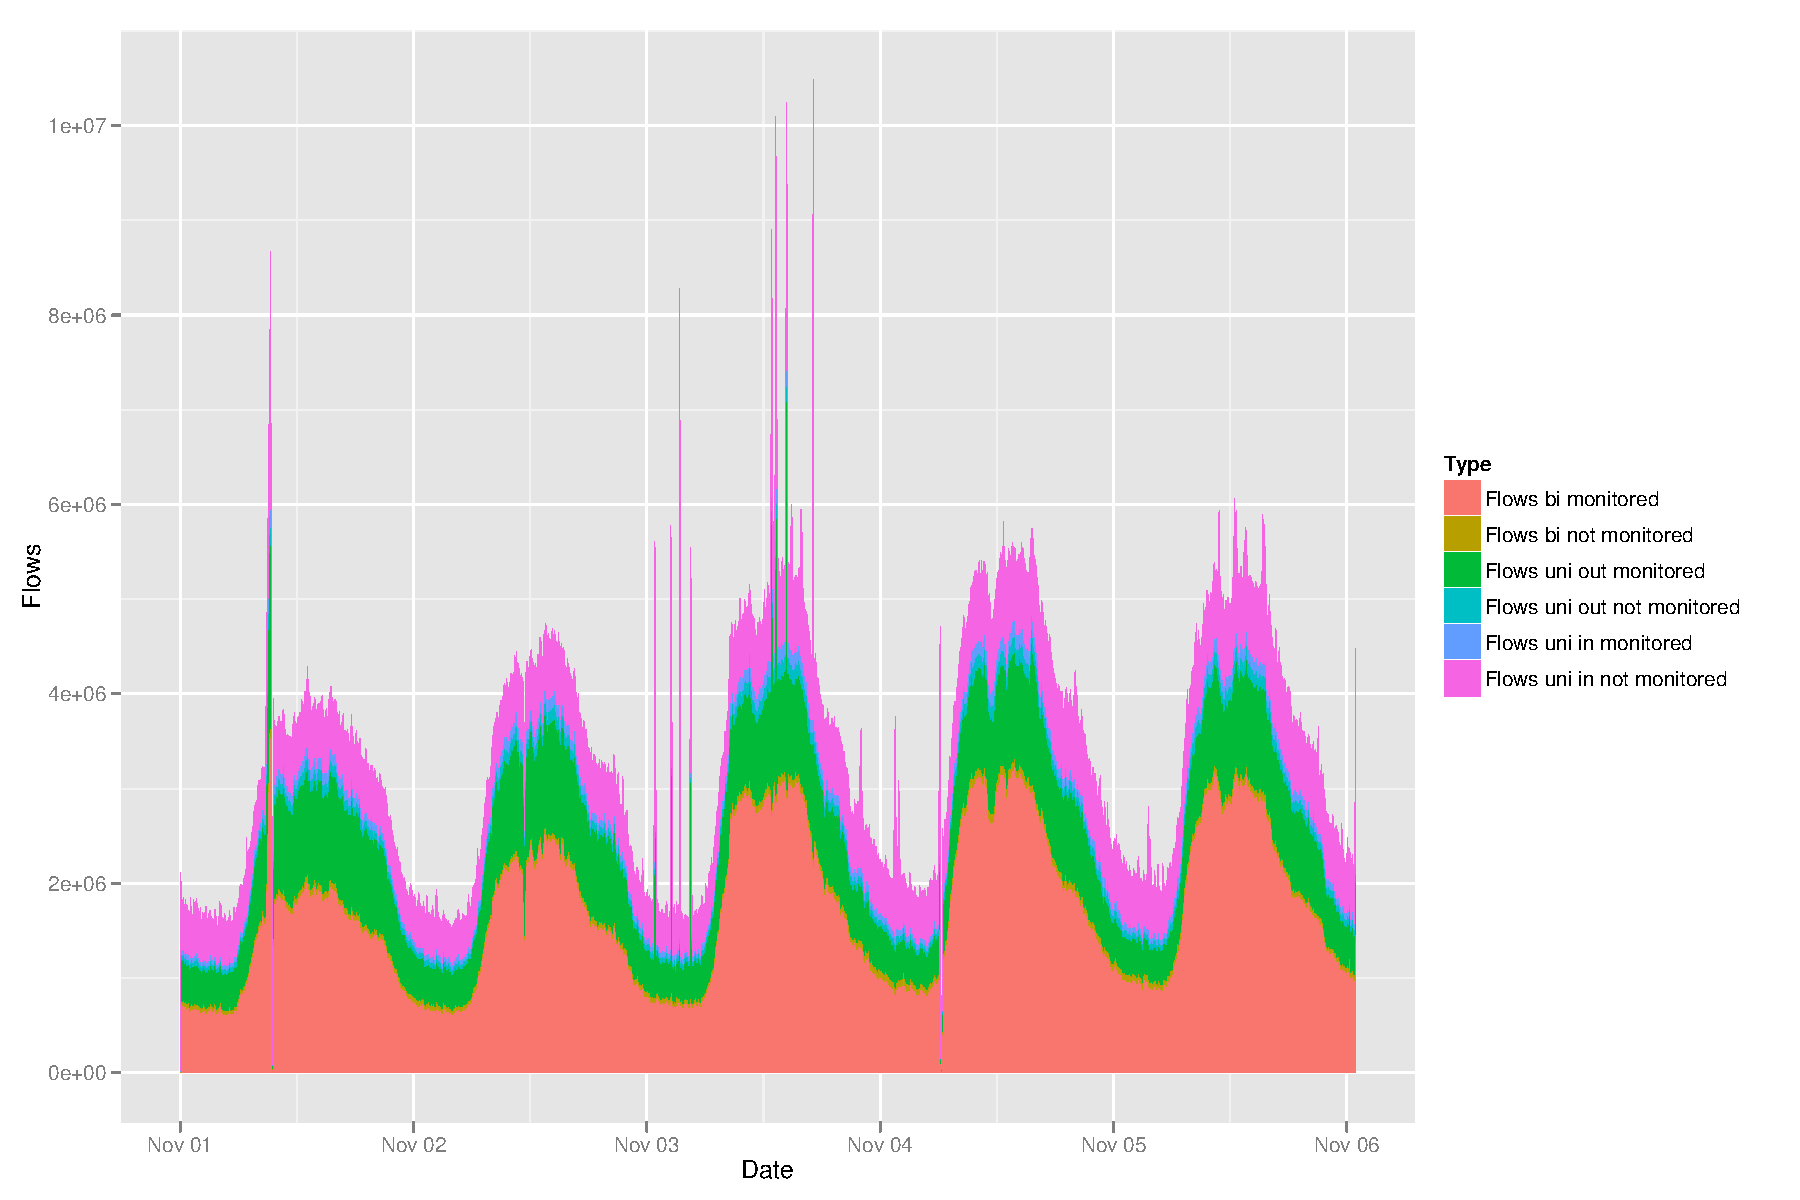
\includegraphics[width=\linewidth]{images/Flows_by_type_area_all_SeS.pdf}
	\caption{Flows by Type} 
	\label{fig:flows_by_type} 
\end{figure}


\begin{figure}
	[ht] \centering 
	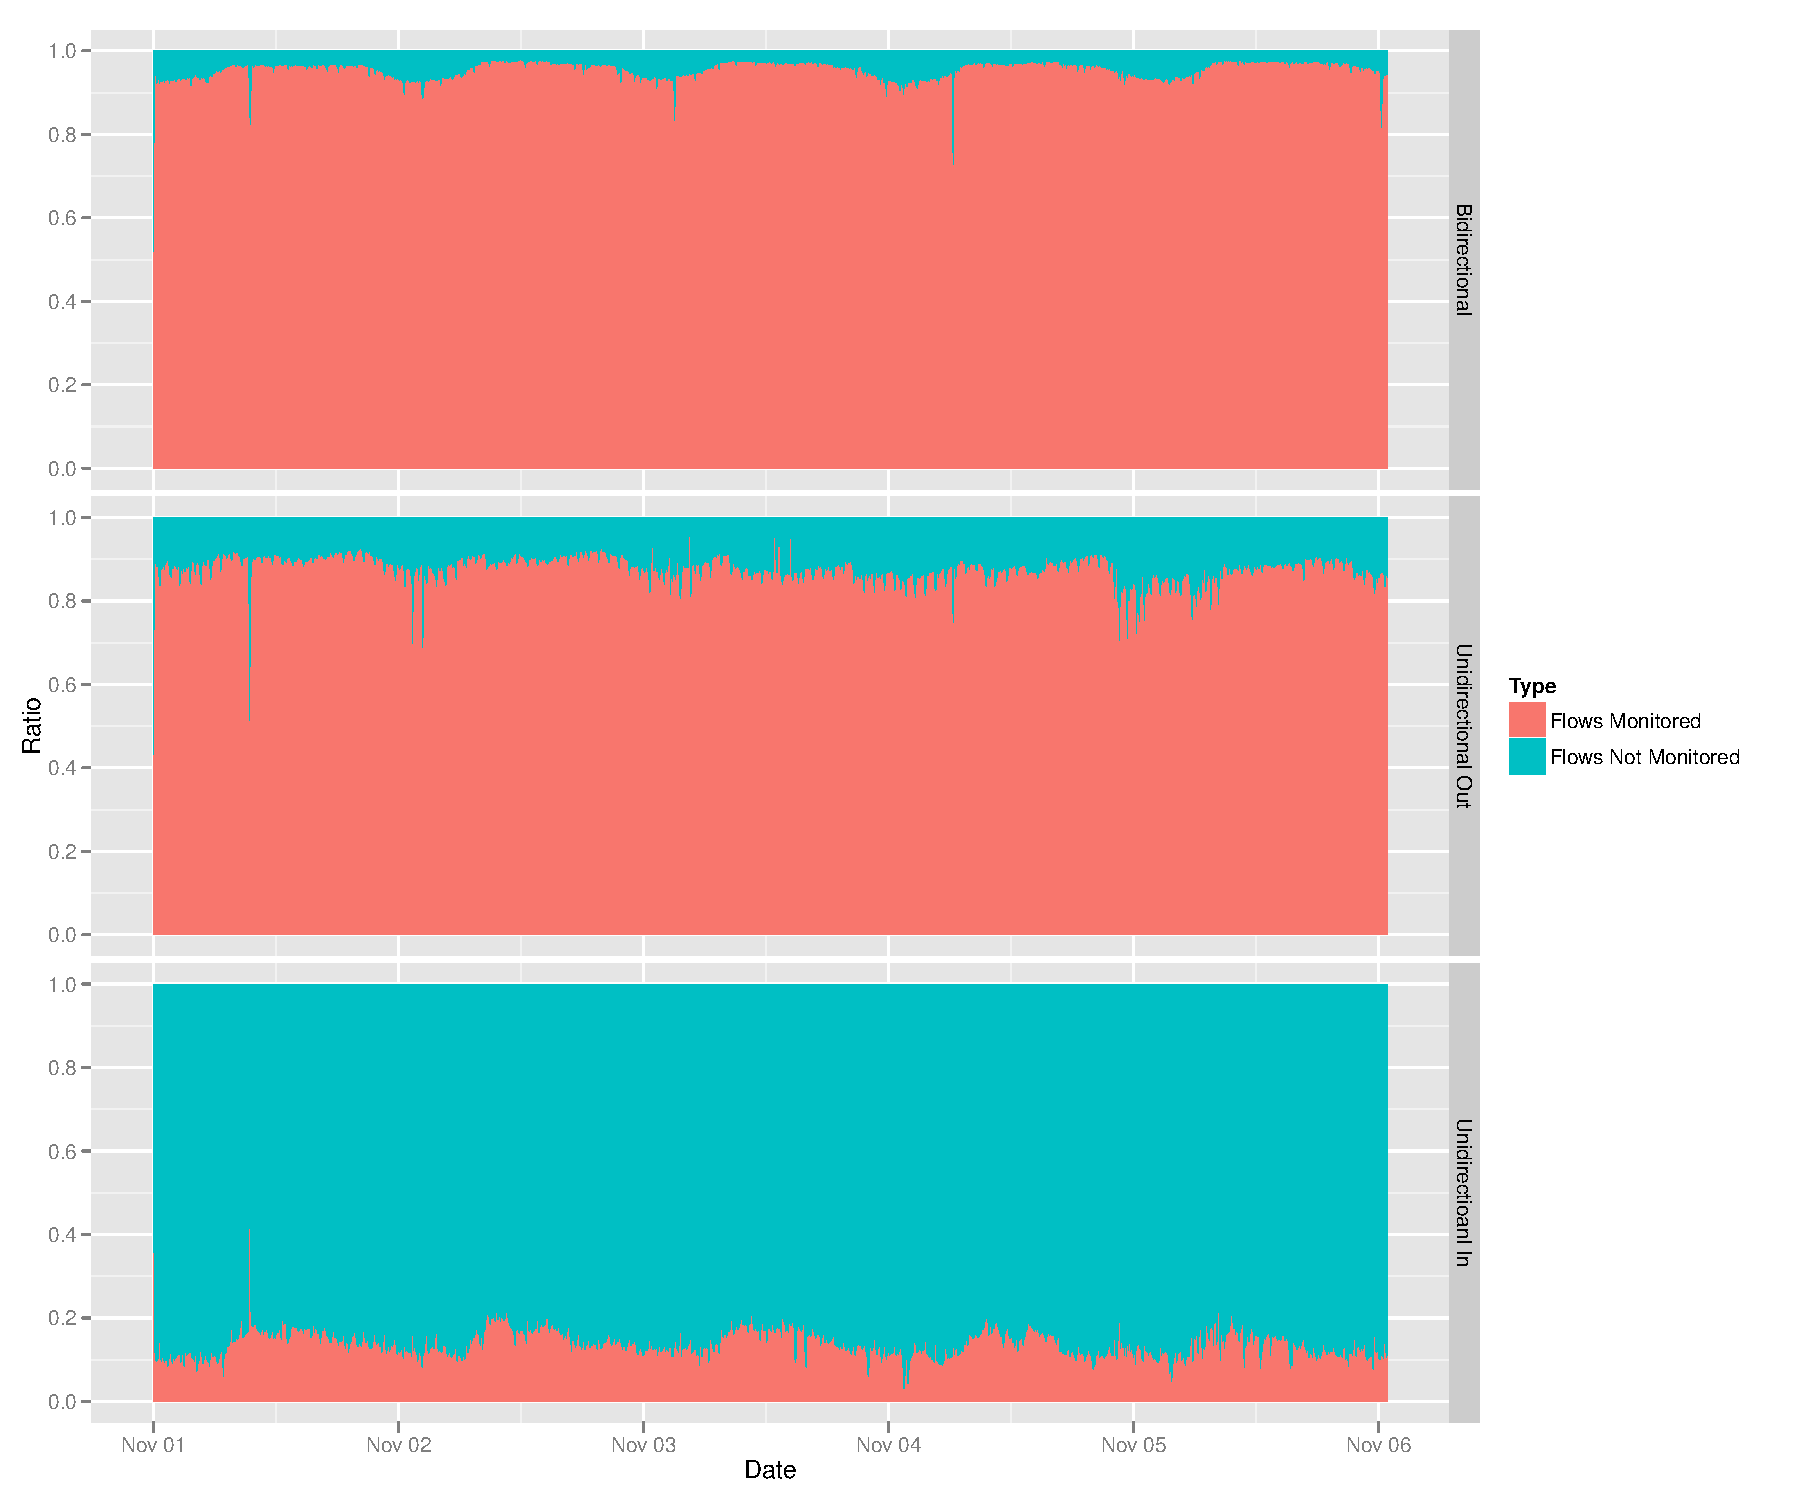
\includegraphics[width=\linewidth]{images/Flows_monitor_ratio_by_type_all_SeS.pdf}
	\caption{Flows towards a detected server socket by type traffic} 
	\label{fig:monitored_flows_by_type} 
\end{figure}


\subsection{Characterization of detected Server Sockets}

\subsubsection{Visibility}
\begin{figure}
	[ht] \centering 
	\includegraphics[width=\linewidth]{images/VTS_by_visibledays.pdf}
	\caption{VTS by visible days} 
	\label{fig:vts_by_visibledays} 
\end{figure}

\subsubsection{Stability}


\begin{landscape}
\begin{figure}
	[ht] \centering 
	\includegraphics[width=\linewidth]{images/CCDF_ratio_days.pdf}
	\caption{CCDF of the availability by visible days} 
	\label{fig:ccdf_ratio_days} 
\end{figure}
\end{landscape}

\begin{landscape}
\begin{figure}
	[ht] \centering 
	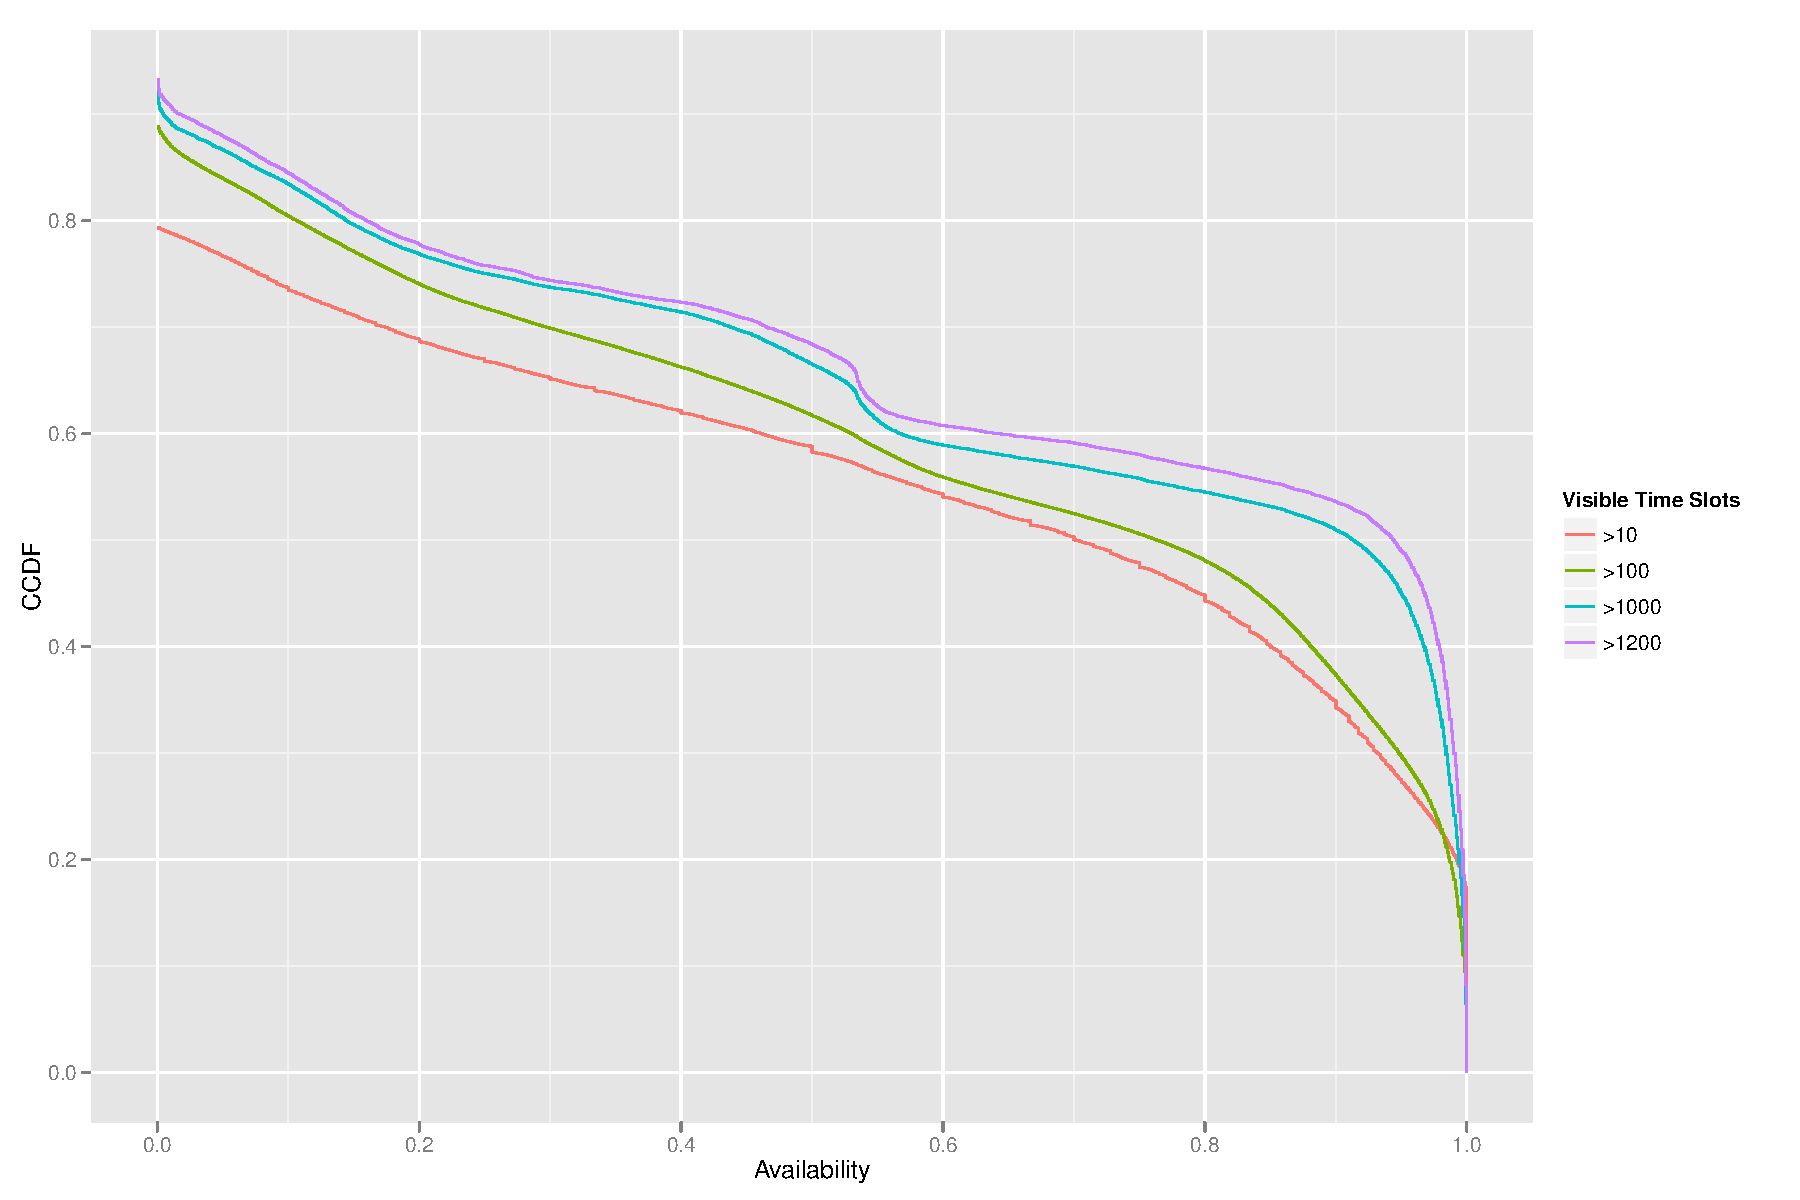
\includegraphics[width=\linewidth]{images/CCDF_ratio_VTS.pdf}
	\caption{CCDF of the availability by visible time slots} 
	\label{fig:ccdf_ratio_vts} 
\end{figure}
\end{landscape}

\subsubsection{Popularity}

\begin{landscape}
\begin{figure}
	[ht] \centering 
	\includegraphics[width=\linewidth]{images/top20_ratio_box.pdf}
	\caption{Boxer plot of the availability / stability of the top 20 traffic port server sockets} 
	\label{fig:top20_ratio_box} 
\end{figure}
\end{landscape}

\begin{landscape}
\begin{figure}
	[ht] \centering 
	\includegraphics[width=\linewidth]{images/top20_visibility_box.pdf}
	\caption{Boxer plot of visibility in days of the top 20 traffic port server sockets}
	\label{fig:top20_visibledays_box}
\end{figure}
\end{landscape}


\begin{table}
	[ht] \centering 
	\begin{tabular}
		{|c|r|r|r|r|r|r|} \hline \textbf{Position} & \textbf{Port} & \textbf{Protocol} & \textbf{Flows} &\textbf{ Flows in \%} & \textbf{Sockets} & \textbf{Sockets in \%}\\
		\hline \hline 1 & 53 & 17 &793851107 & 47.272216 & 314253 & 18.68397\\
		\hline 2 & 80 & 6 &623910956 & 37.152626 & 546735 & 32.50623\\
		\hline 3 & 443 & 6 & 74333936 & 4.426434 & 59800 & 3.555420\\
		\hline 4 & 22 & 6 & 10580812 & 0.630066 & 40363 & 2.399790\\
		\hline 5 & 2703 & 6 & 10139578 & 0.603791 & 22 & 0.001308\\
		\hline 6 & 25 & 6 & 6943533 & 0.413473 & 18560 & 1.103488\\
		\hline 7 & 123 & 17 & 4988781 & 0.297072 & 286 & 0.017004\\
		\hline 8 & 993 & 6 & 3844043 & 0.228905 & 1398 & 0.083118\\
		\hline 9 & 555 & 6 & 3290709 & 0.195955 & 9 & 0.000535\\
		\hline 10 & 995 & 6 & 2411245 & 0.143585 & 654 & 0.038884\\
		\hline 11 & 110 & 6 & 1816240 & 0.108153 & 1211 & 0.072000\\
		\hline 12 & 3789 & 6 & 1796224 & 0.106961 & 10 & 0.000595\\
		\hline 13 & 53 & 6 & 1726716 & 0.102822 & 1102 & 0.065520\\
		\hline 14 & 2128 & 6 & 1677027 & 0.099864 & 390 & 0.023188\\
		\hline 15 & 3478 & 17 & 1607132 & 0.095701 & 176 & 0.010464\\
		\hline 16 & 8080 & 6 & 1362615 & 0.081141 & 2056 & 0.122240\\
		\hline 17 & 3128 & 6 & 1298424 & 0.077319 & 191 & 0.011356\\
		\hline 18 & 5354 & 6 & 1221109 & 0.072715 & 3 & 0.000178\\
		\hline 19 & 8001 & 6 & 1014631 & 0.060419 & 58 & 0.003448\\
		\hline 20 & 21 & 6 & 1010771 & 0.060189 & 1419 & 0.084367\\
		\hline 21 & high & 6 & 37679906 & 2.243762 & 599314 & 35.63233\\
		\hline 22 & high & 17 & 89558306 & 5.333015 & 89820 & 5.340265\\
		\hline 23 & low & 6 & 2505504 & 0.149198 & 3807 & 0.226346\\
		\hline 24 & low & 17 & 749276 & 0.044618 & 302 & 0.017955\\
		\hline 
	\end{tabular}
	\caption{Top 20 port / protocol aggregated sockets by number flows} 
\end{table}

SSH TCP 22: Scanning / PW guessing, e.g. X.X.X.X, 6, 22, 1.0, 2, 1, 69.0, 0.0, 0.0 always with 69 or 68 biflows (parallelized? recurring?) $\rightarrow$ that's way such a bad visibility! one-time shots.. /8 network is scanned! meist 3-4 timeslots und nur visibility einem Tag! 

mDNS (5354) $\rightarrow$ Apple mdns resolving; mainly one socket causing this traffic pm-members.apple.com
%
%!TEX root = ./main.tex
%** 50_integration.tex
\chapter{Extending FACT with Server Sockets\label{chapter:integration}}

%%%%%%%%%%%%%%%%%%%%%%%%%%%%%%%%%%%%%%%%%%%%%%%%%%%%%%%%%%%%%%%%%%%%%%%%%%%%%%%%
% Smart Traffic Selection using Server Sockets Sets
%%%%%%%%%%%%%%%%%%%%%%%%%%%%%%%%%%%%%%%%%%%%%%%%%%%%%%%%%%%%%%%%%%%%%%%%%%%%%%%%
\section{Smart Traffic Selection using Server Sockets Sets\label{section:ses_traffic_selection}}
% explain briefly the approach / adjustments to FACT
Originally, \gls{FACT} applies a port-based heuristic for selecting the 
examination traffic. 
In detail, \gls{FACT} selects in a first step all traffic towards an external 
\gls{TCP} port 80 originated from an internal client high port. 
Generally, this kind of traffic is denoted as the reflector traffic. 
Then, \gls{FACT} examines each connection from the reflector traffic if it is 
balanced or unbalanced, thus creating an initial set of potential events. 

\begin{figure}
	[!b] \centering
	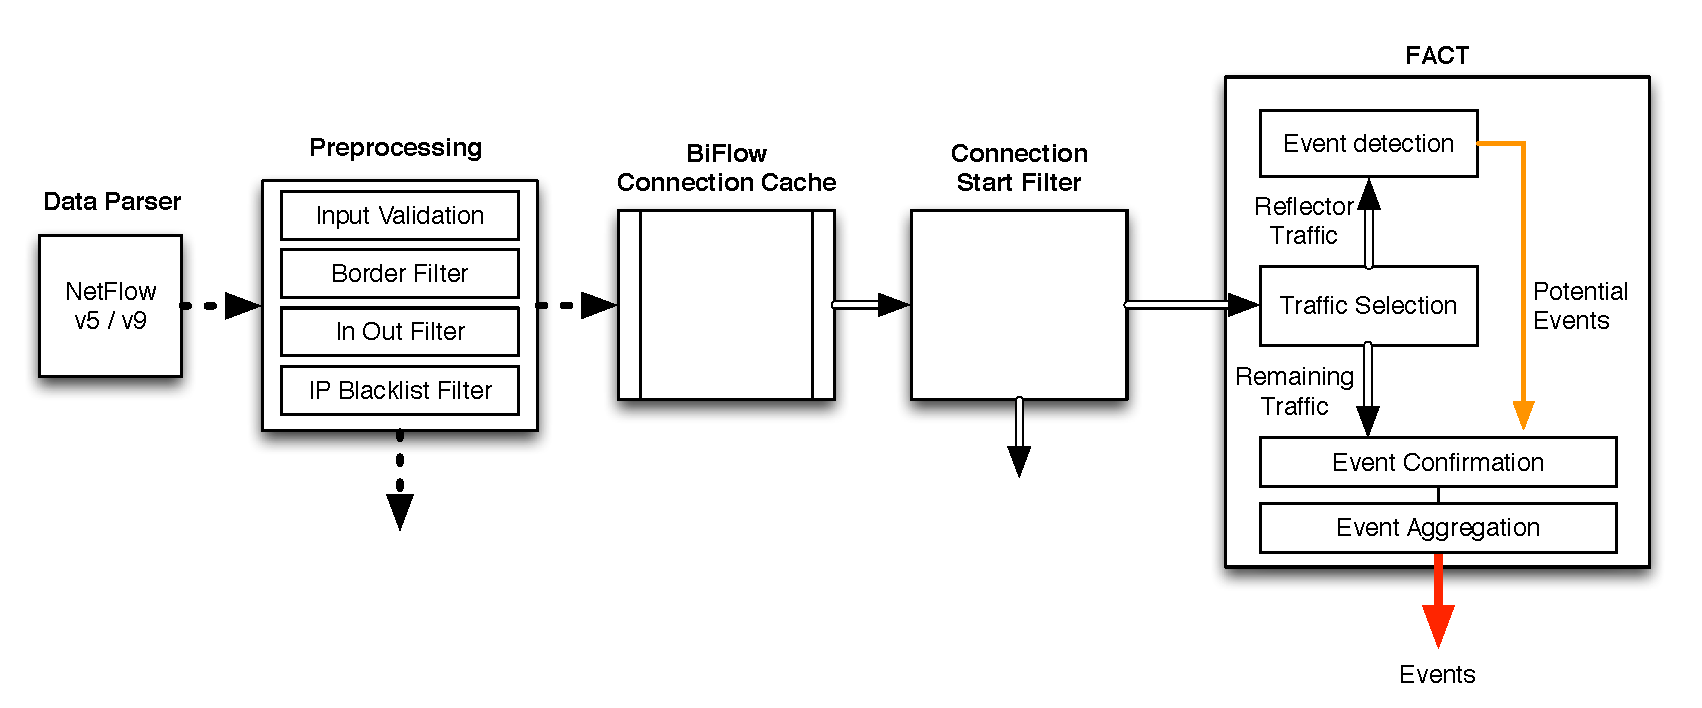
\includegraphics[width=\linewidth]{images/FACT.eps}
	\caption{Processing chain for FACT} 
	\label{fig:fact_chain} 
\end{figure}

In a second step, all potential events inferred by the reflector traffic are 
double-checked with the remaining traffic if a potential event is indeed a 
event. Only if there are no successful connections at all, i.e. all connections 
are unbalanced, a host, network or prefix is declared as unreachable. Otherwise, 
if there is other traffic towards these hosts, networks, and prefixes with 
balanced connections, the potential event is obviously not confirmed and thus 
removed from the event list. 

Since the \gls{server socket} approach aims to replace the port-based heuristic, 
only the generation of the reflector traffic set must be adjusted. The further 
processing steps remain exactly the same. Figure \ref{fig:fact_chain} 
illustrates the \gls{FACT} processing chain and makes clear that only the block 
of the traffic selection must be adjusted to examine traffic towards 
\glspl{server socket} as reflector traffic. This is achieved by loading the 
\gls{server socket} registry with a set of \glspl{server socket}. Then, the 
adjusted traffic selection is querying the server socket registry if the 
external socket is a known \gls{server socket}. If this is the case, the flow is 
added to the reflector traffic, otherwise to the remaining traffic. 

\section{Optimal Server Sockets Sets\label{section:ses_selection}}
% outline that this is a optimization problem which is approximated by several 
% socket sets however not guaranteed to be optimal
% coverage network space / problem space 
By adjusting the traffic selection of \gls{FACT} with \gls{server socket} sets, some essential properties of \gls{FACT} as the observed network coverage or the event sensibility are directly dependent on properties of the chosen 
\gls{server socket} set. 

Because \gls{FACT} detects only network outage events which are firstly detected with the reflector traffic and then not whitelisted by the remaining traffic, it is able to detect only network outages of prefixes which have at least one known 
server socket that is located in this prefix. This means that FACTs observation 
coverage of networks is completely defined by the network/prefix coverage of the 
chosen \gls{server socket} set. 

Obviously, it makes no sense to select for example the 10 most popular sockets 
if they are all located in the same network and prefix, because this set would 
just achieve a network coverage of 1 network/prefix. Hence, the network coverage 
can be optimized by selecting the best socket of these 10 and then select 9 
different sockets which are all located in different networks/prefixes. By doing 
so, the network coverage can be increased. However, if a selected 
\gls{server socket} is not contacted during an observation period the 
observation coverage of this network is lost, unless there is another contacted 
socket located in this network. 
This shows that the selection of \glspl{server socket} is cumbersome and 
directly influences the observation capabilities of FACT. It also shows the 
importance of the visibility and popularity characteristics of \glspl{server socket} 
with respect to the selection in a \gls{server socket} set. 

A popular \gls{server socket} which is always contacted by at least one client 
is able to cover the entire network, because even if this socket is not 
reachable during an observation period the network is further investigated by 
the remaining traffic. 
This is because the unbalanced connection of this \gls{server socket} 
will trigger a potential event which is then confirmed or whitelisted by the 
remaining traffic towards this network. Otherwise, if a socket is not popular 
and only rarely visible, it will not generate a potential event, and hence, the 
event is not detected at all, even if there is a lot of unbalanced traffic 
towards this network contained in the remaining traffic. 

Therefore, the selection of the \glspl{server socket} is basically an optimization 
problem. The goal is to select those sockets with good stability, popularity and 
visibility characteristic without loosing to much network coverage. This problem 
can even be harder if the number of sockets is limited, then the socket density 
of each network must be considered, so that only the few best sockets located in 
a single network are selected. It can even make sense to include not perfectly 
stable sockets if they increase the network coverage, especially if they have a 
good visibility / popularity.


%%!TEX root = ./main.tex

%** Results.tex: What were the results achieved including an evaluation

\chapter{Results and Evaluation\label{Results}}

\section{Results}
\subsection{IPv6 and the SWITCH network\label{RES_IPV6}}
\begin{figure}[hb!]
	\centering
	\includegraphics[height=70mm]{images/overview_v4v6}
	\caption{Comparison of the traffic levels of IPv4 and IPv6 in the SWITCH network in terms of connections per 5 minutes}
	\label{fig:ipv6_switch}
\end{figure}
This section is to get an idea of the deployment of IPv6 in the SWITCH network at the end of August 2010. As figure \ref{fig:ipv6_switch} shows that there are around 8M-20M IPv4 connections per 5 min time slot. On the other hand, there are only 50k-100k IPv6 connections per 5 min time slot. So the overall traffic level of IPv4 is a factor 160 - 200 higher than the traffic level of IPv6. This means that there is at least 160 times more IPv4 traffic than IPv6 traffic. Consequently, FACT has some trouble in detecting connectivity issues in IPv6 networks with the same reliability as in IPv4 networks because of this significant lower traffic volume, i.e. most likely due to a significant lower number of IPv6 user.

\subsection{Analysis of a two week traffic trace}
In order to demonstrate how efficient and comfortable FACT works in practice, a few details of a two week traffic trace from the entire SWITCH network are elaborated. This traffic trace has started on 30/08/2010 at midnight and ended around 12 days later on 11/09/2010. Since FACT is analyzing the data split up in 5 minute time slots, there are 3492 reporting files generated.

\subsubsection{Data}
SWITCH is collecting unsampled traffic traces at their boarder router which exports netflow traces to a central instance within the SWITCH network. They are saved so that these traces are available for several years back. The CSG has an exclusive access to this traffic traces in order to a research contract with SWITCH.

\subsubsection{IPv4}
A brief statistic of this two week IPv4 traffic trace:
\begin{itemize}
	\item 2170 time slots are classified as \texttt{UNLIKELY}, this yields that there are no problems reported in 62\% of the time (180 hours within 291 hours).
	\item 912 time slots are classified as \texttt{LIKELY}. In 26\% of the cases there may be a connectivity issue. However, some further investigation is required to definitely denote a connectivity problem within these time slots.
	\item 410 time slots are classified as \texttt{VERY LIKELY}. Hence, in 34 hours (11\%) of the trace a connectivity issue is reported.
\end{itemize}

Figure \ref{fig:ipv4_prefix_failed} is presenting the number of failed prefixes over time. This semi-log plot shows how many external prefixes are classified as unreachable over time. The severity is indicated by colors, red stands for $severity \ge 1$ which means that at least one host is affected by the given number of failed prefixes. According to that, green stands for $severity \ge 2$, blue for $severity \ge 5$ and purple for $severity \ge 10$. It is visible that the red curve is heavily fluctuating, because there is a high impact of some noise like port scans, DDoS backscatter, etc. Consequently, the green curve is showing the number of failed external prefix whose outage affects two or more internal hosts. This is to be considered as more robust to noise. Therefore, if at least 10 internal hosts are affected one is attempted to state that this is certainly a real connectivity problem. Hence, for each purple spot there may be a connectivity issue on a very high probability.
\begin{figure}[hb!]
	\centering
	\includegraphics[height=75mm]{images/prefix_failed_ipv4.eps}
	\caption{number of failed IPv4 prefixes within the two week traffic trace}
	\label{fig:ipv4_prefix_failed}
\end{figure}

\subsubsection{IPv6}
Figure \ref{fig:ipv6_prefix_failed} is showing again how many external prefixes are classified as unreachable, but for IPv6 instead of IPv4 as in figure \ref{fig:ipv4_prefix_failed}. Obviously, there are hardly any IPv6 connectivity issues detected in contrast to the IPv4 plot. This may be a result of the low traffic level of IPv6 in the SWITCH network or just because there are no severe connectivity issues within the observed timeframe. The red spots which can be seen on figure \ref{fig:ipv6_prefix_failed} are prefix failures which only affect one internal host and this is - as stated above - not very reliable. Moreover, there are five green spots which indicate a prefix failure which affects 2 or more internal hosts. Further investigation though yields that these spots are caused by the same two hosts within a single /48 network. This may be a real connectivity issue. However, only two internal hosts are affected by this problem which is of course still not as reliable as severity 10.

\begin{figure}[hb!]
	\centering
	\includegraphics[height=80mm]{images/prefix_failed_ipv6.eps}
	\caption{number of failed IPv6 prefixes within the two week traffic trace}
	\label{fig:ipv6_prefix_failed}
\end{figure}

\section{Evaluation}
As the two plots above shows, prefix failures may be extracted quite well with FACT. So further investigation of the problematic time instances is needed. This may be done through the consultation of the report file of these time slots. At 30/08/2010 11.15 CEST for example there are 4 IPv4 prefixes reported as failed with $severity \ge 10$ . The investigation yields that some prefixes of a content distribution network provider have not been reachable during 2 hours and thus, caused that some content of this provider and their customers were partially unavailable. The larger purple blocks around the 08/09/2010 till the 11/09/2010 exhibits again one of these prefixes as broken. This shows that it was not possible to completely resolve that problem within at least 12 days. If FACT were deployed at that moment, this prefix failure, which may be a result of a broken peering or another routing failure, would have been resolved faster.

This analysis of the two week trace shows how easy it is to classify and identify connectivity issues with FACT. However, FACT requires a certain level of traffic to reliably classify connectivity issues. Moreover, there are some methodical details to evaluate:
\begin{itemize}
	\item How precise is the classification of connectivity issues?
	\item How complete is the classification of connectivity issues?
	\item How low is the false positive rate?
\end{itemize}

\subsection{Precision}
The precision is defined as the fraction of the true positives and the sum of the true positives and the false positives. Further investigation of the report files and of the above plot yields that there are hardly any False Positives in this data set which leads to a very low false positive. Therefore, the Precision should be quite high, at least if there is enough traffic to get a high severity.

\subsection{Recall}
The recall is an indicator for the completeness of the connectivity issue tracking. Firstly, the complete set of connectivity issues has to be defined. Either all connectivity issues of the entire Internet are defined as set of connectivity issues or all connectivity issues which concern the network users. In the first case the recall would be very low, because it is very unlikely that the connections of all internal users will track all connectivity issues in the entire Internet. Consequently, there are a lot of false negatives and therefore, the recall is very low. The second case is harder to examine and needs a very detailed examination which will not fit the extent of this thesis. This is due to the uncertainty of how robust and reliable the severity one is. If all connectivity issues of severity one are considered, the false negatives will increase by this amount what decreases the recall in turn.

\subsection{False Positive Rate}
To determine the false positive rate the robustness and significance of the severity has to be estimated again. Since the consideration of severity one will lead to a high number of false positives due to port scans or other blocked traffic, the false positive rate will be higher than in the cases of severity bigger than one. This assumes that the likelihood of independently creating scanning traffic or some blocked traffic towards the same external network by two or more internal hosts is very low. Nevertheless, relying on a severity bigger than one should lead to a quite low false positive rate. However, there is a conflict between the false positive rate and the recall. The overall traffic level impacts again the ability to aggregate prefix failures by internal hosts. The higher the traffic level is, the higher the probability to aggregate a prefix failure to more than one host and the more reliable a classification gets.

%%!TEX root = ./main.tex
\chapter{Conclusion\label{Conclusion}}

\section{Conclusion}
Adjusting the traffic preselection of FACT from a port-based heuristic to a 
server socket based approach is far more than just a generalization. 

On the one hand, the server sockets approach is less affected by scanning and 
p2p, acting as a kind of history based scanning filter. Thus, reducing the 
negative effect of malware and p2p churn on the network outage detection. 

On the other hand, a smart composition of the server socket set used for the 
detection process may generally increase the observation coverage of FACT 
without significantly increasing the noise ratio. Hence, the practical usability 
of FACT is increase even more.

The drawback of the approach is clearly the additional resources required to 
store the server sockets and the additional effort to detect, monitor and 
characterize the server sockets. Nevertheless, the good results from chapter 
\ref{chapter:results} indicates that server sockets are quite stable over time 
and that there are even good results possible for events in March, May and 
August 2010 with sockets detected in November 2010. 

However, the selection of server sockets can be cumbersome and directly 
influences the detection sensitivity of FACT. Though, even without any 
optimization the server socket approach is clearly outperforming the original port-based heuristic with respect to the \emph{event-to-noise} ratio. 

\section{Future Work}
% characterize ses by time based activity (night / day, working week, weekend etc.)

% smarter socket set selection => density of network by choosing only the popularst sockets of each network

% automatization of process => danger of excluding sockets affected by events
% => consider full last week?  

% general optimization problem solving approach as simulated annealing => limit number of sockets => pareto front of sockets

% consider different selection methods as clustering analysis approaches, e.g. k-means etc => distance function include also network considerations.. etc. 

% near future public release of FlowBox and FACT

% LIST of Figures and Tables
\listoffigures
\listoftables

% Appendix-mode in Latex
\appendix

% Set enumeration to alphabetical  characters.
\renewcommand{\thepart}{\Alph{part}}
%!TEX root = ./main.tex

\chapter{Appendix}
\label{appendix}
\section{Prefix Files for FACT}

Switchextract is a neat little perl script for generating the required prefix files for the FilterInOut and the Analyser of FACT. It may be found in the tool folder of the FACT sourcecode. For correctly using these perl script, the following preliminary work have to be done:
\begin{enumerate}
	\item Download and install bgpdump from the RIPE RIS project.
	\item Download the bgpdump file of the desired date from a suitable route collector - the best from the default free rrc00.ripe.net.
	\item Adjust your own AS number within the perl script switchextract.pl, i.e. replace 559 at line 24 with your own AS number.
\end{enumerate}

Then the following steps must be executed:
\begin{enumerate}
	\item Create a file bgpdump.txt with bgpdump: \newline\texttt{bgpdump bview.XXXXXX.XXXX.gz -m > bgpdump.txt}
	\item Call the perl script switchextract.pl: \newline\texttt{perl switchextract.pl bgpdump.txt prefixes.txt}
	\item prefixes.txt has to be moved or linked to the analyser configuration folder of FACT
	\item switch\_prefixes.txt is needed by the FilterInOut and has to be moved or linked to the configuration folder of FilterInOut.
\end{enumerate}


%** Originalproblem.tex: The problem statement you received.
%!TEX root = ./main.tex
\newpage
\section{Problem Description}

\includegraphics[width=\linewidth, page=1]{ThesisDescription.pdf}
\newpage
\includegraphics[width=\linewidth, page=2]{ThesisDescription.pdf}
\newpage
\includegraphics[width=\linewidth, page=3]{ThesisDescription.pdf}

%!TEX root = ./main.tex
\bibliographystyle{apalike} 
\bibliography{95_bib}



%!TEX root = ./main.tex
\chapter*{Eigenständigkeitserklärung} Ich erkläre hiermit, dass es sich bei
der von mir eingereichten schriftlichen Arbeit mit dem Titel
\textbf{"Identification of Connectivity Issues in Large Networks using Data
Plane Information"} um eine von mir selbständig und in eigenen Worten verfasste
Originalarbeit handelt.\\

\vspace{5mm} \textbf{Verfasser:}\\
Daniel Aschwanden\\

\vspace{5mm} \textbf{Betreuer:}\\
Dominik Schatzmann\\
Wolfgang Mühlbauer\\

\vspace{5mm} Mit meiner Unterschrift bestätige ich, dass ich über fachübliche
Zitierregeln unterrichtet worden bin und das Merkblatt
(\url{http://www.ethz.ch/students/exams/plagiarism_s_de.pdf}) gelesen und
verstanden habe. Die im betroffenen Fachgebiet üblichen Zitiervorschriften sind
eingehalten worden.
Eine Überprüfung der Arbeit auf Plagiate mithilfe elektronischer Hilfsmittel
darf vorgenommen werden.\\

\vspace{15mm} 
\begin{tabular}
	{l p{0.3
	\textwidth} r} Zürich, 11.03.2011 &&
	Daniel Aschwanden \\
\end{tabular}

\vfil

\end{document}

%%% Local Variables:
%%% mode: latex
%%% TeX-master: "documentation"
%%% End: